% Para definir o tipo de documento, descomente apenas
% uma das linhas "\documentclass" abaixo

% comentar uma linha significa colocar "%"
% descomentar uma linha significa remover o "%"

%\documentclass[msc]{on}     % dissertação de mestrado
\documentclass[dsc]{on}     % tese de doutorado
%\documentclass[dscexam]{on} % exame de qualificação
%\documentclass[reportd]{on} % relatório feito durante o doutorado
%\documentclass[reportm]{on} % relatório feito durante o mestrado

% pacotes utilizados
\usepackage[utf8]{inputenc}
\usepackage{amsmath,amssymb}
\usepackage{hyperref}
\usepackage{enumerate} %para gerar listas numeradas
\usepackage{graphicx}  %para figuras eps
\usepackage{subfigure} %para figuras múltimas, com (a), (b), (c), etc.
\usepackage[english, ruled]{algorithm2e}
\usepackage{pdfpages}
\usepackage{float}

% os dois comandos estão com problema e deverão ser
% corrigidos futuramente
%\makelosymbols
%\makeloabbreviations

\begin{document}
  	
  % Título em português
  \title{Inversão Magnética em diferentes escalas}
  
  % Título em inglês
  \foreigntitle{Magnetic Inversion at different scales}
  
  % Autor
  \author{André Luis}{Albuquerque dos Reis}

  % Orientador(a)
  \advisor{Dr.}{Vanderlei}{Coelho de Oliveira Junior}
  %\advisor{Dr.}{Nome do orientador}{Sobrenome}

  % Co-orientadores (pode ser mais de um)
  \coadvisor{Dra.}{Valéria Cristina}{Ferreira Barbosa}
  %\coadvisor{Dr.}{Nome do Co-orientador}{Sobrenome}

  % Examinadores (caso seja um relatório, não modifique as linhas "\examiner")
  %\examiner{Dra.}{Nome da Examinadora}{Sobrenome}
  %\examiner{Dr.}{Nome do Examinador}{Sobrenome}
  %\examiner{Dra.}{Nome da Examinadora}{Sobrenome}
  %\examiner{Dr.}{Nome do Examinador}{Sobrenome}
  %\examiner{Dra.}{Nome da Examinadora}{Sobrenome}

  % Programa de Pós-Graduação 
  \program{GEO}
    
  % Data (mês e ano)
  \date{11}{2019}

  % Palavras-chave
  \keyword{Primeira palavra-chave}
  \keyword{Segunda palavra-chave}
  \keyword{Terceira palavra-chave}

  \maketitle

  %\begin{abstract}
A tecnica da camada equivalente é comumente utilizada no processamento de dados de anomalia de campo total estimando uma distribuição de momentos magnéticos 2D composta por dipolos abaixo do plano de observação. No entanto, algumas técnicas de processamento que utilizam a camada equivalente dependem do conhecimento da direção de magnetização das fontes. Neste trabalho, investigamos dois aspectos teóricos e práticos da técnica da camada equivalente. No primeiro deles, desenvolvemos um método para estimar a direção de magnetização total das fontes magnéticas baseado na técnica da camada equivalente utilizando dados de anomalia de campo total. Quando a direção de magnetização das fontes equivalentes são próximas da direção de magnetização das fontes verdadeiras, a propriedade magnética sobre a camada é inteiramente positiva. Iterativamente, o método proposto impõe a regularização de Tikhonov de ordem zero e um vínculo de positividade sobre os momentos magnéticos estimados e estimam a direção de magnetização das fontes geológicas. Matematicamente, o algoritmo resolve um problema de mínimos quadrados em dois passos: o primeiro resolvendo um problema inverso linear para estimar uma distribuição de momentos magnéticos 2D sobre a camada e o segundo resolvendo um problema inverso não-linear para a direção de magnetização das fontes magnéticas. Na segunda abordagem, testamos se a aplicação da técnica da camada equivalente no cálculo das componentes e da amplitude do campo magnético depende da direção de magnetização das fontes. Fixamos uma direção de magnetização e estimamos uma distribuição de momentos magnéticos que pode ser utilizada para calcular as componentes do campo magnético e sua amplitude. Em ambos os casos, esta abordagem não requer informações sobre a geometria ou profundidade das fontes, e nem dados regularmente espaçados. Testamos a metodologia proposta aplicando a dados sintéticos para diferentes cenários geológicos, e os resultados mostram que o método pode ser uma ferramenta poderosa para estimar a direção de magnetização de um conjunto de fontes. Teste com dados de campo na província alcalina de Goiás (PAGO), região central do Brasil, sobre o complexo de Montes Claros sugerem que estas intrusões possuem fortes componentes de magnetização remanente, que está em acordo com a literatura atual para esta região. Além disso, testamos a técnica de processamento com dados sintéticos simulando amostras de rocha, e os resultados mostram que este tipo de processamento não depende do conhecimento prévio da magnetização de magnetização. Utilizando dados de microscopia magnética, a aplicação deste tipo de processamento em uma amostra geológica proveniente da cratera de Vredefort confirma esta característica da camada equivalente.
\end{abstract}   % resumo em português - deve ser utilizado por todos os tipos de documento
  %\begin{abstract}
It is known from potential theory that a continuous and planar layer of dipoles can exactly reproduce the total-field anomaly produced by arbitrary 3D sources. We show that, if the magnetization direction of this layer is the same as that of the true sources, its magnetic-moment distribution is all positive. This property holds true regardless of whether the magnetization of the true sources is purely induced or not. By using this generalized positivity constraint, we present a new iterative method for estimating the total magnetization direction of 3D magnetic sources based on the equivalent-layer technique. Our method does not impose a priori information either about the shape or depth of the sources, does not require regularly spaced data and presumes that the sources have a uniform magnetization direction. At each iteration, our method performs two steps. The first one solves a constrained linear inverse problem to estimate a positive magnetic-moment distribution over a discrete equivalent layer of dipoles. We consider that the equivalent sources are located on a plane and have an uniform and fixed magnetization direction. The second step uses the estimated magnetic-moment distribution and solves a nonlinear inverse problem for estimating a new magnetization direction for the dipoles. The algorithm stops when the equivalent layer yields a total-field anomaly that fits the observed data. Tests with synthetic data simulating different geological scenarios show that the final estimated magnetization direction is close to the true one. We applied our method to a field data from the Goi{\' a}s Alkaline Province (GAP), over the Montes Claros complex, center of Brazil. The result suggests the presence of intrusions with remarkable remanent magnetization, in agreement with the current literature for this region.
\end{abstract} % resumo em inglês - deve ser utilizado por todos os tipos de documento
  \tableofcontents   % sumário - deve ser utilizado por todos os tipos de documento
  \listoffigures     % lista de figuras
  %\listoftables      % lista de tabelas

  % os dois comandos estão com problema e deverão ser
  % corrigidos futuramente
  %\printlosymbols
  %\printloabbreviations

  \mainmatter
  
%%% corpo do texto

%% Introdução 
\chapter{Introdução}
\label{chap:introducao}

A maioria dos métodos magnéticos requerem o conhecimento da direção de magnetização, caso contrário produzem informações insatisfatórias sobre as fontes. Este fato tem impulsionado o desenvolvimento de diversas técnicas para estimar a direção de magnetização ao longo dos últimos 50 anos. As estratégias para estimar esta quantidade podem ser dividida em dois grupos principais. O primeiro grupo compreende aqueles métodos que presumem informações prévias acerca da geometria das fontes. O método iterativo apresentado por \cite{bhattacharyya1966} presume que as fontes magnéticas tem formato de prismas retangulares. \cite{emilia_massey_1974} aproxima um monte submarino por um conjunto de prismas justapostos com direção de magnetização uniforme e intensidade variável. \cite{parker_etal_1987} aproximam a geometria de um monte submarion utilizando uma cobertura de faces triangulares e estimam a magnetização interna próxima a uma solução uniforme. \cite{parker_etal_1987} apresentaram um método que estima a direção de magnetização total e a orientação espacial de uma fonte isolada que possui três planos ortogonais de simetria. \cite{kubota2005} aproximaram também um monte submarino por um conjunto de prismas justapostos, mas estimaram a direção de magnetização para cada um dos prismas. Finalmente, \cite{oliveirajr_etal_2015} aproximam as fontes magnéticas por corpos esféricos de centros conhecidos e estimam suas direções de magnetização. O segundo grupo é formado pelos métodos que não presumem informações sobre a geometria das fontes. \cite{fedi_etal_1994}, por exemplo, propôs um método que determina a melhor direção de magnetização dentre um conjunto de tentativas usadas para realizar sucessivas reduções ao polo no domínio de Fourier. \cite{phillips2005} utilizaram integrais de Helbig para estimar as componentes do vetor de momento magnético. \cite{tontini_pedersen_2008} extenderam o método de Phillips utilizando as mesmas integrais de Helbig para estimar a direção de magnetização e sua magnitude, e fornecendo informações sobre a posição do centro de distribuição de magnetização. \cite{lelievre_oldenburg_2009} desenvolveram um método para estimar a direção de magnetização em cenários geológicos complexos. Este método aproxima a subsuperfície por um grid de prismas justapostos e estima as componentes do vetor magnetização para cada prisma. Além destes métodos, existem aqueles que são baseados na correlação de quantidades potenciais \citep[e.g.,][]{dannemiller_li_2006,gerovska_etal_2009,liu_etal_2015,zhang_etal_2018}. 

Estimar a direção de magnetização é extremamente importante não só para interpretação, mas também para o processamento de anomalia de campo total. Uma técnica no domínio do espaço comumente utilizada para esta finalidade é a camada equivalente. Esta técnica foi introduzida na geofísica de exploração por \cite{dampney1969} e \cite{emilia_massey_1974} para o processamento de dados gravimétricos e magnéticos, respectivamente. Após estes trabalhos pioneiros, esta técnica tem sido vastamente utilizada para realizar interpolação \citep{cordell_1992, mendonca-silva_1994, barnes-lumley_2011, siqueira_etal_2017}, continuação para cima (ou para baixo) \citep{hansen_miyazaki_1984, li-oldenburg_2010}, redução ao polo \citep{silva_1986, leao-silva_1989, guspi-novara_2009, oliveirajr-etal_2013}, calcular a amplitude do campo anômalo \citep{li_li_2014} e para filtrar ruídos de dados de gradiometria \citep{martinez_li_2016}. A técnica da camada equivalente consiste em aproximar um conjunto de dados observados por dados produzidos por uma camada composta de fontes discretas (e.g., prismas, dipolos ou pontos de massa), que são comumente conhecidas como fontes equivalentes. Os dados produzidos por esta camada fictícia (a camada equivalente) são chamados de dados preditos. 

Em microscopia magnética, a técnica da camada equivalente é geralmente utilizada para a interpretação da distribuição de momentos magnéticos em uma lâmina de rocha. Note que, neste caso, a camada equivalente se assemelha a fonte verdadeira (a lâmina de rocha). \cite{weiss2007} apresentou um dos primeiros trabalhos utilizando a camada equivalente em microscopia magnética. Os autores apontaram que a distribuição de magnetização é interamente positiva se a direção de magnetização das fontes equivalentes é igual a direção utilizada para uma amostra de rocha magnetizada artificialmente. \cite{baratchart2013} mostraram matematicamente que, assumindo uma direção de magnetização uniforme, o problema inverso para estimar a distribuição de momentos magnéticos é único. \cite{lima2013} propôs um método no domínio da frequência para investigar soluções tendo a direção de magnetização uniforme iguais a das lâminas de rocha. Eles mostraram empiricamente que, neste caso, a distribuição de momentos magnéticos na camada é inteiramente positiva.  Em geofísica de exploração, a camada equivalente é predominantemente utilizada para o processamento de dados potenciais. Neste sentido, não existe relação entre a distribuição de propriedade física estimada sobre a camada equivalente e as fontes geológicas verdadeiras. Poucos autores tem direcionado o uso da camada equivalente para a interpretação de fontes geológicas. \cite{pedersen1991}, por exemplo, discutiu a relaçao entre o campo potencial e a fonte equivalente. \cite{medeiros_silva1996} e \cite{silvadias_etal_2010} estimaram um mapa de magnetização aparente sobre a camada utilizando regularizações de Tikhonov e entrópica, respectivamente. \cite{siqueira_etal_2017} estabeleceu a relação entre o excesso de massa estimado sobre a camada e o verdadeiro. \cite{li_etal_2014} provaram, utilizando uma abordagem no domínio de Fourier, a existência de uma distribuição de momentos magnéticos positiva sobre a camada e utilizaram esta propriedade para contornar o problema de instabilidade em baixas latitudes. No entanto, estes autores consideraram somente um caso particular no qual as fontes magnéticas tenham magnetização puramente induzida. 

Neste trabalho, provamos matematicamente que a distribuição de momentos magnéticos positiva sobre a camada equivalente existe mesmo que a magnetização das fontes verdadeiras seja remanente. Esta distribuição positiva de momentos magnéticos é válida para todos os casos nos quais a direção de magnetização das fontes equivalentes tem a mesma direção das fontes verdadeiras, mesmo que a magnetização destas fontes seja puramente induzida ou não. Amparado neste vínculo de positividade generalizado, apresentamos um método iterativo que usa a técnica da camada equivalente para estimar a direção de magnetização uniforme de fontes arbitrárias invertendo dados de anomalia de campo total. Nosso método não presume qualquer informação sobre a geometria das fontes. A cada iteração nosso método resolve (1) um problema linear, sujeito a um vínculo de positividade para estimar a distribuição de momentos magnéticos sobre uma camada de dipolos e (2) um problema inverso não-linear para estimar a direção de magnetização uniforme das fontes equivalentes. Testes com dados sintéticos gerados por cenários geológicos diferentes mostram que a direção de magnetização estimada converge para a direção verdadeira das fontes verdadeiras. Aplicamos também nosso método a dados de campo provenientes da província alcalina de Goiás, sobre o complexo de Montes Claros, na região central do Brasil. Nosso resultado está de acordo com os resultados obtidos por \cite{zhang_etal_2018} para a mesma área, sugerindo a presença de marcantes componentes de magnetização remanente e mostrando a boa performance do nosso método na interpretação de cenários geológicos complexos. 



%% Metodologia (desenvolvimento teórico para as duas partes do projeto)
\chapter{Metodologia}
\label{chap:metodologia}

\section{Estimativa das componentes e da amplitude do campo magnético}
\label{sec:componentes_campo}

Na seção \ref{sec:Gauss-Ampere}, mostrei que, se uma camada equivalente plana 
com direção de magnetização uniforme e arbitrária 
reproduz uma determinada componente $B_{\alpha}(x, y, z)$ (equação \ref{eq:B-alpha-true-generic}),
$\alpha = x, y, z$, do campo de indução magnética $\mathbf{B}(x, y, z)$ (equação \ref{eq:B-true-generic}) 
produzido por um conjunto de fontes magnéticas arbitrárias, esta camada deve, 
obrigatoriamente, reproduzir as demais componentes do campo $\mathbf{B}(x, y, z)$.
Nesta seção, apresento um método para estimar as componentes e a amplitude do campo de indução 
magnética de um conjunto de fontes magnéticas a partir da inversão de dados de uma determinada 
componente.

\subsection{Parametrização e problema direto}
\label{subsec:balpha_prob_dir}

Considere uma camada equivalente plana localizada em $z = z_{c}$, que possui uma distribuição 
contínua de intensidades de momento magnético $p(x'',y'',z_{c})$ e uma direção de magnetização 
arbitrária $\hat{\mathbf{u}}(I, D)$ (equação \ref{eq:B-alpha-layer}). 
Em situações práticas, não é possível determinar esta distribuição contínua de intensidade de momentos 
sobre a camada equivalente. 
Por esta razão, a camada é aproximada por um conjunto discreto de $M$ dipolos (fontes equivalentes) 
localizados no plano $z = z_{c}$ (Figura \ref{fig:eqlayer_balpha_sketch}).
A componente $\alpha$, $\alpha = x, y, z$, do campo de indução magnética produzida por esta camada 
discreta (componente $\alpha$ predita) no ponto $(x_{i},y_{i},z_{i})$, $i=1,\dots,N$, é dada por 
\begin{equation}
B^{\alpha}_{i} (\mathbf{p})  = \mathbf{g}^{\alpha}_{i}(\mathbf{q})^{\top} \, \mathbf{p},
\label{eq:B-alpha-pred-i}
\end{equation}
em que $\mathbf{q}$ é um vetor $2 \times 1$ (vetor de direção de magnetização) definido 
em termos da inclinação e declinação ($I$ e $D$) da magnetização total na camada equivalente
\begin{equation}
\mathbf{q} = \begin{bmatrix}
I \\ D 
\end{bmatrix} \: ,
\label{eq:q-vector}
\end{equation}
$\mathbf{p}$ é um vetor $M \times 1$ (vetor de momentos magnéticos) cujo $j$-ésimo elemento, $j=1,\dots,M$, 
é a intensidade do momento magnético $p_{j}$ (em $A \, m^{2}$) do $j$-ésimo dipolo e 
$\mathbf{g}^{\alpha}_{i}(\mathbf{q})$ é outro vetor $M \times 1$ cujo $j$-ésimo elemento é definido pela 
função harmônica 
\begin{equation}
g_{ij}^{\alpha}(\mathbf{q})  = \gamma_{m} \, {\mathbf{M}^{\alpha}_{ij}}^{\top} \, \hat{\mathbf{u}}(\mathbf{q}) \: .
\label{eq:g_ij-alpha}
\end{equation}
Nesta equação, $\hat{\mathbf{u}}(\mathbf{q}) \equiv \hat{\mathbf{u}}(I, D)$ é um vetor unitário
definido pela equação \ref{eq:u-hat} em função da inclinação e declinação 
da magnetização na camada equivalente ($I$ e $D$) e $\mathbf{M}^{\alpha}_{ij}$ é um vetor $3 \times 1$ 
dado por 
\begin{equation}
\mathbf{M}^{\alpha}_{ij} = \begin{bmatrix}
\partial_{\alpha x} \frac{1}{r''} \\
\partial_{\alpha y} \frac{1}{r''} \\
\partial_{\alpha z} \frac{1}{r''}
\end{bmatrix} \quad ,
\label{eq:Mij-matrix-alpha}
\end{equation}
em que $\partial_{\alpha\beta} \frac{1}{r''} \equiv \frac{\partial^{2}}{\partial \alpha \partial \beta} \frac{1}{r''}$ 
representa a segunda derivada da função $\frac{1}{r''}$ (equação \ref{eq:inv-r''}) em relação a $\alpha$ e $\beta$, 
$\alpha = x, y, z$, $\beta = x, y, z$, avaliada nas coordenadas $(x, y, z) = (x_{i}, y_{i}, z_{i})$ do $i$-ésimo dado  
observado e $(x'', y'', z_{c}) = (x_{j}, y_{j}, z_{c})$ da $j$-ésima fonte equivalente.
A componente $\alpha$ predita $B^{\alpha}_{i} (\mathbf{p})$ (equação \ref{eq:B-alpha-pred-i}) é 
obtida a partir da discretização da integral que define a componente $\tilde{B}_{\alpha}(x, y, z)$
(equação \ref{eq:B-alpha-layer}) produzida pela camada equivalente contínua.
Note que $B^{\alpha}_{i}(\mathbf{p})$ possui uma relação linear com o vetor de momentos 
magnéticos $\mathbf{p}$.

%% Figura
\begin{figure}[H]
	\centering
	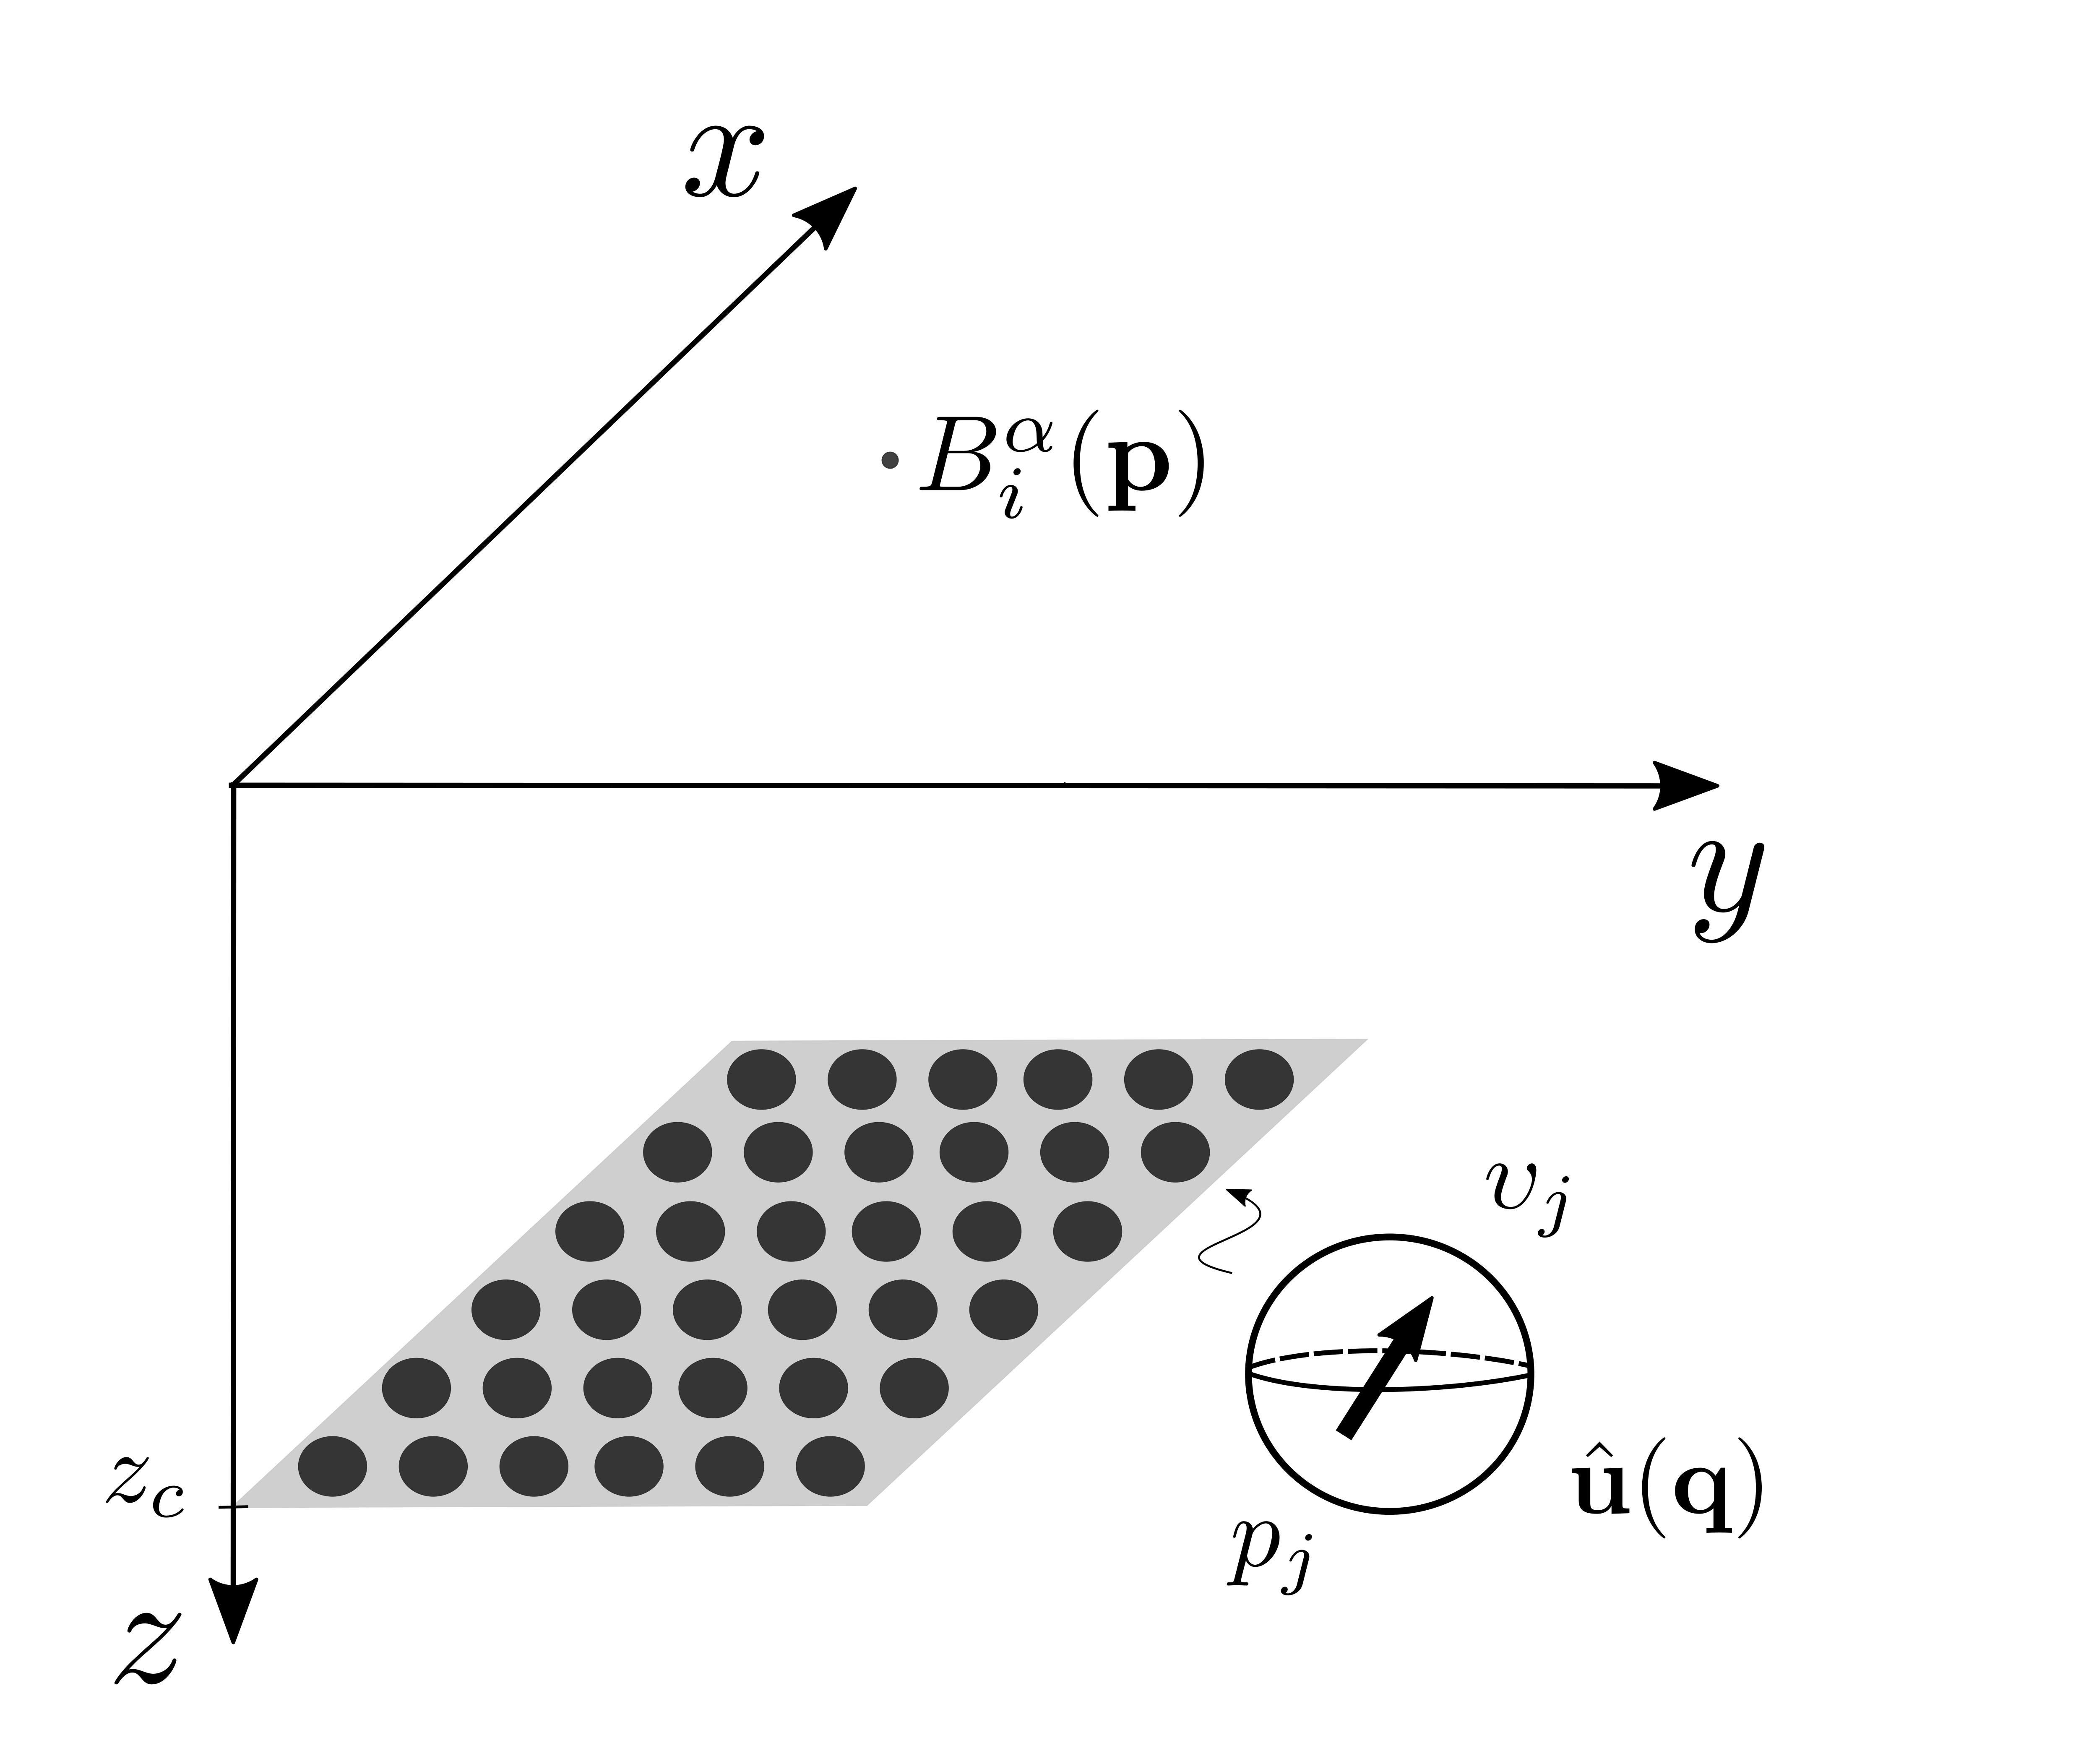
\includegraphics[width=.7\textwidth]{Fig/mag_vec/eqlayer_figure_balpha.png}
	\caption{Representação esquemática da camada equivalente para a componente $\alpha$ do campo de 
	indução magnética. A camada é posicionada sobre o plano horizontal $z = z_{c}$. 
	$B^{\alpha}_{i}(\mathbf{p})$ é a componente $\alpha$ predita (equação \ref{eq:B-alpha-pred-i}) no 
	ponto $(x_{i},y_{i},z_{i})$ pelo conjunto de $M$ fontes equivalentes (pontos pretos). 
	Cada fonte é localizada em um ponto  $(x_{j},y_{j},z_{c})$, 
	$j = 1,\dots, M$, e é representada por um dipolo de volume unitário $\upsilon_{j}$ 
	com direção de magnetização $\hat{\mathbf{u}}(\mathbf{q})$ e momento magnético $p_{j}$.}
	\label{fig:eqlayer_balpha_sketch}
\end{figure}

\subsection{Problema inverso}
\label{subsec:balpha_prob_inv}

Seja $\mathbf{B}^{\alpha}_{o}$ o vetor de dados observados cujo $i$-ésimo elemento é a componente 
$\alpha$, $\alpha = x, y, z$, do campo magnético produzida por fontes magnéticas arbitrárias no ponto 
$(x_{i},y_{i},z_{i})$, $i = 1, \dots, N$. Similarmente, seja $\mathbf{B}^{\alpha}(\mathbf{p})$ 
o vetor de dados preditos cujo $i$-ésimo elemento é a componente $\alpha$ predita 
$B^{\alpha}_{i} (\mathbf{p})$ (equação \ref{eq:B-alpha-pred-i}) produzida por uma camada equivalente 
discreta no mesmo ponto $(x_{i},y_{i},z_{i})$. 
Para estimar o vetor de momentos magnéticos $\mathbf{p}$ que minimiza a diferença entre 
$\mathbf{B}^{\alpha}_{o}$ e $\mathbf{B}^{\alpha}(\mathbf{p})$, minimizo a seguinte função 
objetivo
\begin{equation}
\Psi(\mathbf{p}) =\lVert \mathbf{B}^{\alpha}_{o} - \mathbf{B}^{\alpha}(\mathbf{p}) 
\rVert_{2}^{2} + \, \mu  \parallel \mathbf{p} \parallel_{2}^{2} \: ,
\label{eq:goal_function_vec}
\end{equation}
em que o primeiro e o segundo termo da equação \ref{eq:goal_function_vec} são a função de ajuste e a 
função regularizadora de Tikhonov de ordem zero, $\mu$ é o parâmetro de regularização e 
$\| \cdot \|_{2}^{2}$ representa o quadrado da norma Euclidiana. 
Usando uma direção de magnetização $\hat{\mathbf{u}}(\mathbf{q})$ (equação \ref{eq:g_ij-alpha}) arbitrária,
a minimização da função objetivo $\Psi(\mathbf{p})$ (equação \ref{eq:goal_function_vec}) resulta no 
sistema linear abaixo:
\begin{equation}
\left[ {\mathbf{G}^{\alpha}}^{\top} \mathbf{G}^{\alpha} + \mu \, \mathbf{I} \right] 
\bar{\mathbf{p}} = {\mathbf{G}^{\alpha}}^{\top} \mathbf{B}^{\alpha}_{o} \: ,
\label{eq:linear_sys_p_alpha}
\end{equation}
em que $\mathbf{G}^{\alpha}$ é uma matriz de dimensão $N \times M$ cujo elemento $ij$ é dado pela função 
harmônica $g_{ij}^{\alpha}(\mathbf{q})$ (equação \ref{eq:g_ij-alpha}), avaliada para um vetor de direção 
de magnetização $\mathbf{q}$ (equação \ref{eq:q-vector}) arbitrário, e $\mathbf{I}$ é a matriz identidade 
de ordem $M$. Usando a distribuição de momentos magnéticos $\bar{\mathbf{p}}$ estimada pelo 
sistema linear \ref{eq:linear_sys_p_alpha}, as outras componentes do campo magnético predito pela 
camada equivalente são calculadas escolhendo-se os $\alpha$ correspondentes nas equações 
\ref{eq:B-alpha-pred-i} -- \ref{eq:Mij-matrix-alpha}. 
Por fim, usando as três componentes $B^{\alpha}_{i}(\bar{\mathbf{p}})$
(equação \ref{eq:B-alpha-pred-i}), $\alpha = x, y, z$, calculo a amplitude do campo de indução 
magnética produzido pela camada equivalente discreta em cada ponto $ (x_{i}, y_{i}, z_{i}) $, 
$i = 1, \dots, N$, da seguinte forma:
\begin{equation}
B_{i}(\bar{\mathbf{p}}) = \sqrt{[B^{x}_{i}(\bar{\mathbf{p}})]^{2} + 
[B^{y}_{i}(\bar{\mathbf{p}})]^{2} + [B^{z}_{i}(\bar{\mathbf{p}})]^{2}} \: .
\label{eq:amplitude_field}
\end{equation}

\section{Estimativa da direção de magnetização}
\label{sec:mag_dir_est}

Na seção \ref{sec:distribuicao-positiva}, mostrei que, para uma camada equivalente plana 
reproduzir a anomalia de campo total $\Delta T(x, y, z)$ (equação \ref{eq:Delta-T-true-mag-uniform}) 
produzida por um conjunto de fontes magnéticas com direção de magnetização uniforme, a sua distribuição 
de intensidades de momento magnético $p(x'', y'', z_{c})$ 
deve ser toda positiva (equação \ref{eq:positivity_prop}). Nesta seção, apresento um método 
iterativo que usa este vínculo de positividade dos momentos magnéticos para estimar a direção de 
magnetização uniforme das fontes magnéticas a partir da inversão de dados de anomalia de campo total.

\subsection{Parametrização e problema direto}
\label{subsec:mag_dir_prob_dir}

Considere uma camada equivalente plana localizada em $z = z_{c}$, que possui uma distribuição 
contínua de intensidades de momento magnético $p(x'',y'',z_{c})$ (equação \ref{eq:B-alpha-layer}). 
Em situações práticas, não é possível determinar esta distribuição contínua sobre a camada equivalente. 
Por esta razão, a camada é aproximada por um conjunto discreto de $M$ dipolos (fontes equivalentes) 
localizados no plano $z = z_{c}$ (Figura \ref{fig:eqlayer_tfa_sketch}). 
A anomalia de campo total produzida por esta camada 
discreta (anomalia de campo total predita) no ponto $(x_{i},y_{i},z_{i})$, $i=1,\dots,N$, é dada por 
\begin{equation}
\Delta T_{i}(\mathbf{s}) = \mathbf{g}_{i}(\mathbf{q})^{\top} \mathbf{p},
\label{eq:tfa-pred-i}
\end{equation}
em que $\mathbf{s}$ é um vetor $(M + 2) \times 1$ particionado dado por 
\begin{equation}
      \mathbf{s} = \begin{bmatrix}
		\mathbf{p} \\
		\mathbf{q}
	\end{bmatrix} \: ,
	\label{eq:s-vector}
\end{equation}
$\mathbf{q}$ é o vetor de direção de magnetização (equação \ref{eq:q-vector}), 
$\mathbf{p}$ é um vetor $M \times 1$ (vetor de momentos magnéticos) cujo $j$-ésimo elemento, $j=1,\dots,M$, 
é a intensidade do momento magnético $p_{j}$ (em $A \, m^{2}$) do $j$-ésimo dipolo e 
$\mathbf{g}_{i} (\mathbf{q})$ é outro vetor $M \times 1$ cujo $j$-ésimo elemento é definido pela 
função harmônica 
\begin{equation}
g_{ij} (\mathbf{q})  = \gamma_{m} \hat{\mathbf{u}}_{0}^T \, 
\mathbf{M}_{ij} \, \hat{\mathbf{u}}(\mathbf{q}) \: .
\label{eq:g_ij}
\end{equation}
Nesta equação, $\hat{\mathbf{u}}_{0} \equiv \hat{\mathbf{u}}(I_{0}, D_{0})$ e 
$\hat{\mathbf{u}}(\mathbf{q}) \equiv \hat{\mathbf{u}}(I, D)$ são vetores unitários
definidos pela equação \ref{eq:u-hat} em função da inclinação e declinação do 
campo principal ($I_{0}$ e $D_{0}$) e da camada equivalente ($I$ e $D$),
respectivamente, e $\mathbf{M}_{ij}$ é uma matriz $3 \times 3$ dada por 
\begin{equation}
\mathbf{M}_{ij} = \begin{bmatrix}
\partial_{xx} \frac{1}{r''} & 
\partial_{xy} \frac{1}{r''} &
\partial_{xz} \frac{1}{r''} \\
\partial_{xy} \frac{1}{r''} & 
\partial_{yy} \frac{1}{r''} &
\partial_{yz} \frac{1}{r''} \\
\partial_{xz} \frac{1}{r''} & 
\partial_{yz} \frac{1}{r''} &
\partial_{zz} \frac{1}{r''}
\end{bmatrix} \quad ,
\label{eq:Mij-matrix}
\end{equation}
em que $\partial_{\alpha\beta} \frac{1}{r''} \equiv \frac{\partial^{2}}{\partial \alpha \partial \beta} \frac{1}{r''}$ 
representa a segunda derivada da função $\frac{1}{r''}$ (equação \ref{eq:inv-r''}) em relação a $\alpha$ e $\beta$, 
$\alpha = x, y, z$ e $\beta = x, y, z$, avaliada nas coordenadas $(x, y, z) = (x_{i}, y_{i}, z_{i})$ do $i$-ésimo dado  
observado e $(x'', y'', z_{c}) = (x_{j}, y_{j}, z_{c})$ da $j$-ésima fonte equivalente.
A anomalia de campo total predita $\Delta T_{i}(\mathbf{s})$ (equação \ref{eq:tfa-pred-i}) é 
obtida substituindo-se, na equação \ref{eq:Delta-T-layer}, a 
discretização da integral que define a componente $\tilde{B}_{\alpha}(x, y, z)$
(equação \ref{eq:B-alpha-layer}) produzida pela camada equivalente contínua.
As equações $\ref{eq:tfa-pred-i}$-$\ref{eq:Mij-matrix}$ mostram que a anomalia de campo total predita 
$\Delta T_{i}(\mathbf{s})$ possui uma relação linear com o vetor de momentos magnéticos $\mathbf{p}$ e uma 
relação não linear com o vetor de direção de magnetização $\mathbf{q}$ (equação \ref{eq:q-vector}).

%% Figura 

\begin{figure}[H]
	\centering
	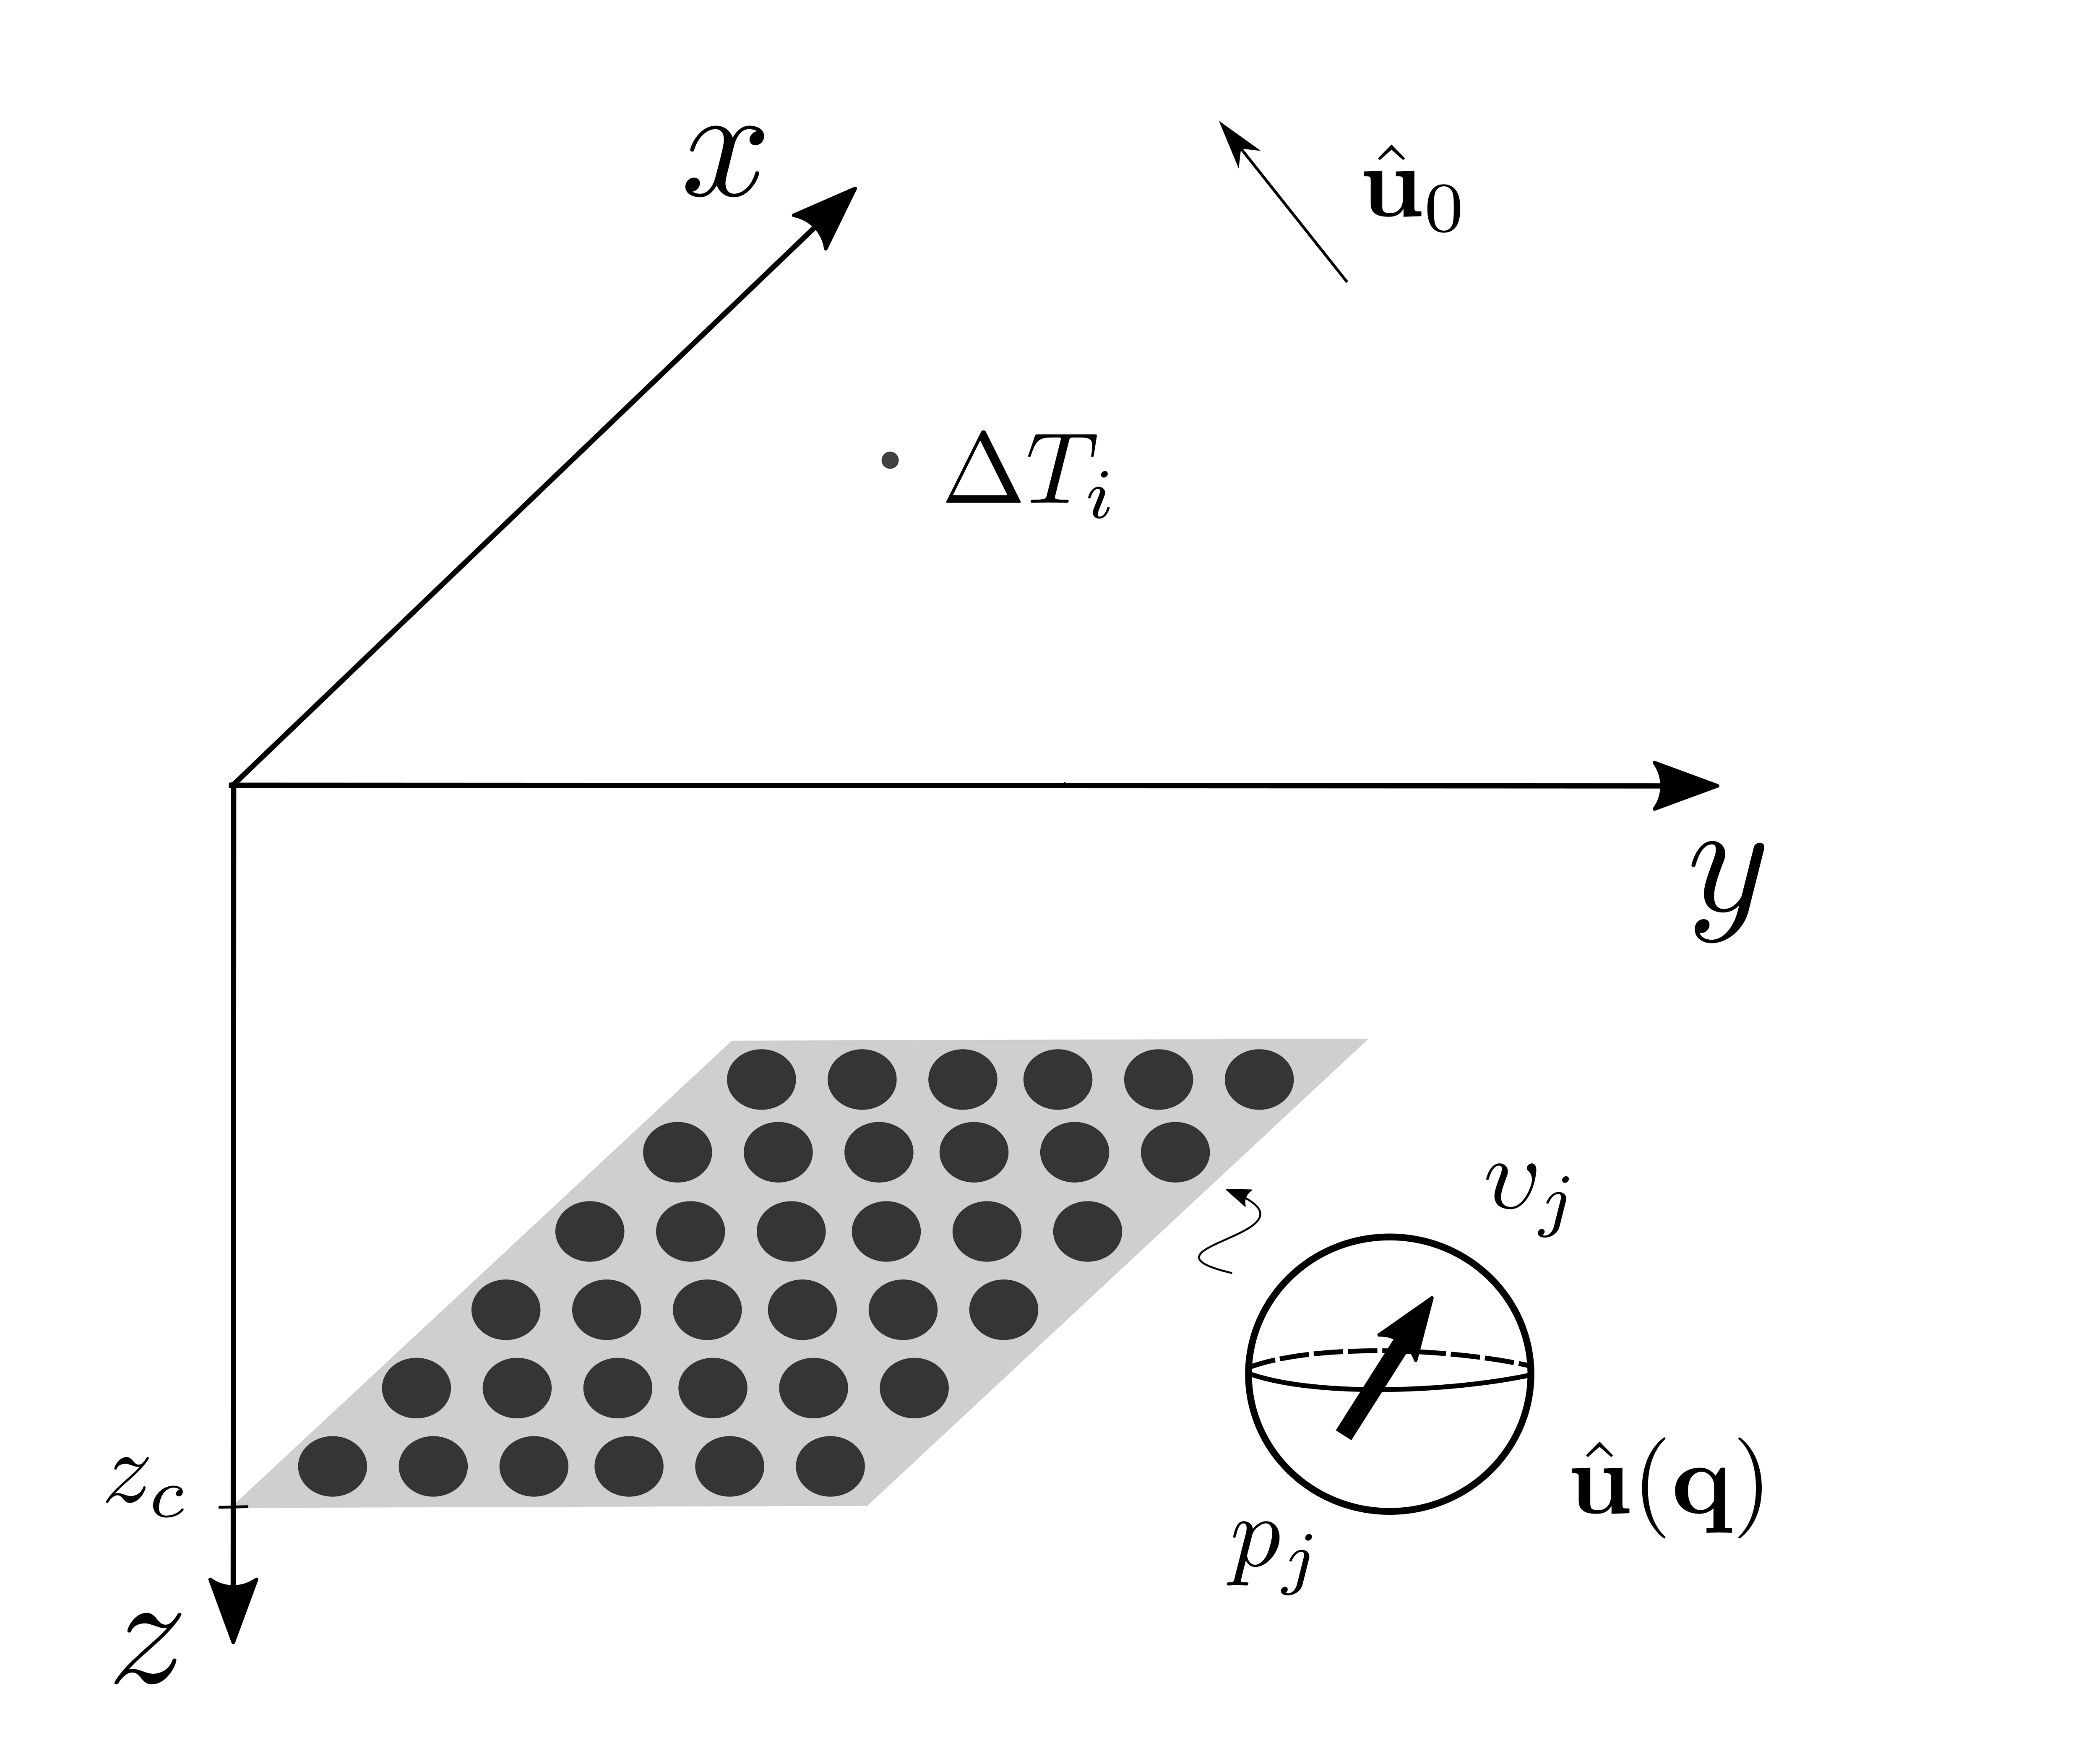
\includegraphics[width=.7\textwidth]{Fig/eqlayer/eqlayer_figure_tfa.png}
	\caption{Representação esquemática da camada equivalente para a anomalia de campo total. A camada é posicionada 
	sobre o plano horizontal a uma profundidade $z=z_{c}$. $\Delta T_{i}(\mathbf{s})$ é a anomalia de campo total predita 
	(equação \ref{eq:tfa-pred-i}) no ponto 
	$(x_{i},y_{i},z_{i})$ produzida pelo conjunto de $M$ fontes equivalentes (pontos pretos). Cada fonte é localizada 
	no ponto  $(x_{j},y_{j},z_{c})$, $j = 1, \dots, M$, e são representadas por um dipolo de volume unitário 
	$\upsilon_{j}$ com direção de magnetização $\hat{\mathbf{u}}(\mathbf{q})$ e momento magnético $p_{j}$. 
	$\hat{\mathbf{u}}_{0} \equiv \hat{\mathbf{u}}(I_{0}, D_{0})$ é um vetor unitário na direção do campo 
	principal.}
	\label{fig:eqlayer_tfa_sketch}
\end{figure}


\subsection{Problema inverso}
\label{subsec:mag_dir_prob_inv}

%%%%% Defining the objective function
Seja $\mathbf{\Delta T}^{o}$ o vetor de dados observados cujo $i$-ésimo elemento é a anomalia de campo 
total produzida, no ponto $(x_{i},y_{i},z_{i})$, $i = 1, \dots, N$, por fontes magnéticas com direção de 
magnetização uniforme. Similarmente, seja $\mathbf{\Delta T} (\mathbf{s})$ o vetor de dados preditos cujo 
$i$-ésimo elemento $\Delta T_{i}(\mathbf{s})$ (equação \ref{eq:tfa-pred-i}) é a anomalia de campo total 
produzida pela camada equivalente discreta no mesmo ponto $(x_{i},y_{i},z_{i})$. 
Para estimar o vetor de parâmetros $\mathbf{s}$ (equação \ref{eq:s-vector}) que minimiza a diferença 
entre $\mathbf{\Delta T}^{o}$ e $\mathbf{\Delta T}(\mathbf{s})$, resolvo o seguinte problema inverso:
\begin{subequations}
	\begin{align}
	& \text{minimizar}
	& &\Psi(\mathbf{s}) =\lVert \mathbf{\Delta T}^{o} - \mathbf{\Delta T} (\mathbf{s}) 
	\rVert_{2}^{2} + \, \mu f_0 \parallel \mathbf{p} \parallel_{2}^{2} \: , \\
	& \text{sujeito a}
	& & p_{j} \geqslant 0 \: , \quad j = 1, \dots, M \: .
	\end{align}
	\label{eq:positivity_goal_function}
\end{subequations}
O primeiro e o segundo termo da equação \ref{eq:positivity_goal_function}a são, respectivamente, a função de ajuste e a função 
regularizadora de Tikhonov de ordem zero, $\mu$ é o parâmetro de regularização, $\| \cdot \|_{2}^{2}$ representa o quadrado da 
norma Euclidiana e $f_{0}$ é um fator de normalização. A equação \ref{eq:positivity_goal_function}b impõe que todos os elementos 
$p_{j}$ do vetor de momentos magnéticos $\mathbf{p}$ sejam maiores ou iguais a zero. 
Este vínculo de positividade se baseia no resultado teórico deduzido na seção \ref{sec:distribuicao-positiva} e 
é incorporado utilizando o \textit{estimador de mínimos quadrados não negativo}, ou NNLS 
(do inglês \textit{Nonnegative least squares}), proposto por \citep{lawson_hanson_1974}.

Para resolver este problema inverso, considere uma expansão até segunda ordem da função $\Psi(\mathbf{s})$
(equação \ref{eq:positivity_goal_function}a) em torno de $\mathbf{s} = \mathbf{s}^{k}$ 
(equação \ref{eq:s-vector}):
\begin{equation}
\Psi(\mathbf{s}^{k} + \mathbf{\Delta s}^{k}) \approx \Psi(\mathbf{s}^{k}) + 
{\mathbf{J}^{k}}^{\top} \mathbf{\Delta s}^{k} + 
\frac{1}{2} {\mathbf{\Delta s}^{k}}^{\top} \mathbf{H}^{k} \mathbf{\Delta s}^{k}  \: ,
\label{eq:sec_ord_goal}
\end{equation}
em que $\mathbf{\Delta s}^{k}$ é uma perturbação no vetor de parâmetros $\mathbf{s}$ 
(equação \ref{eq:s-vector}) e os termos 
$\mathbf{J}^{k}$ e $\mathbf{H}^{k}$ são, respectivamente, o vetor gradiente e a matriz Hessiana avaliadas em $\mathbf{s}^{k}$. 
Calculando o gradiente do lado direito da equação \ref{eq:sec_ord_goal} em relação a $\bar{\mathbf{\Delta s}}^{k}$
e igualando o resultado ao vetor nulo, deduzimos o seguinte sistema linear:
\begin{equation}
\mathbf{H}^{k} \bar{\mathbf{\Delta s}}^{k} = - \mathbf{J}^{k} \: ,
\label{eq:linear_sys_GN}
\end{equation}
que representa o $k$-ésimo passo do método de Gauss-Newton \citep{aster2005} para a minimização da função objetivo (equação \ref{eq:positivity_goal_function}a). Reescrevemos este sistema linear desprezando as derivadas cruzadas na matriz Hessiana como: 
\begin{equation}
\left[
\begin{array}{c|c}
\mathbf{H}_{pp}^{k} & \mathbf{0} \\
\hline
\mathbf{0}^{\top} & \mathbf{H}_{qq}^{k}
\end{array}
\right] \left[ \begin{array}{c}
\bar{\mathbf{\Delta p}}^{k} \\ 
\bar{\mathbf{\Delta q}}^{k} 
\end{array} \right] \approx -\left[ \begin{array}{c}
\mathbf{J}_{p}^{k} \\ 
\mathbf{J}_{q}^{k} 
\end{array} \right] ,
\label{eq:linear_sys_GN_block}
\end{equation}
em que $\mathbf{0}$ é uma matriz $M \times 2$ que contém todos os elementos iguais a zero, 
$\bar{\mathbf{\Delta p}}^{k} = \bar{\mathbf{p}}^{k+1} - \bar{\mathbf{p}}^{k}$ é a correção no vetor de momentos magnéticos 
$\mathbf{p}$, $\bar{\mathbf{\Delta q}}^{k} = \bar{\mathbf{q}}^{k+1} - \bar{\mathbf{q}}^{k}$ é a correção no vetor direção 
de magnetização $\mathbf{q}$ e os termos $\mathbf{J}_{\alpha}^{k}$ e $\mathbf{H}_{\alpha \alpha}^{k}$, $\alpha = p,q$, 
são os vetores gradientes e as matrizes Hessianas calculadas com relação aos elementos de $\mathbf{p}$ e $\mathbf{q}$, 
respectivamente. 

O vetor gradiente $\mathbf{J}_{p}^{k}$ e a matriz Hessiana $\mathbf{H}_{pp}^{k}$ (equação \ref{eq:linear_sys_GN_block}) 
relativos ao vetor de momentos magnéticos $\mathbf{p}$ são, respectivamente, 
\begin{equation}
\mathbf{J}_{p}^{k} = -2 {\mathbf{G}_{p}^{k}}^{\top} 
\left[ \mathbf{\Delta T}^{o} - \mathbf{\Delta T} (\bar{\mathbf{s}}^{k}) \right] + 
2\mu f_{0}^{k} \bar{\mathbf{p}}^{k} 
\label{eq:grad_p}
\end{equation}
e 
\begin{equation}
\mathbf{H}_{pp}^{k} = 2 {\mathbf{G}_{p}^{k}}^{\top} \mathbf{G}_{p}^{k} + 
2 \mu f_{0}^{k} \mathbf{I} \: ,
\label{eq:hess_p}
\end{equation}
em que $\mathbf{G}_p^{k}$ é uma matriz $N \times M$ cujo elemento $ij$ é definido pela função 
harmônica $g_{ij}(\bar{\mathbf{q}}^{k})$ (equação \ref{eq:g_ij}) avaliada na direção de magnetização 
$\bar{\mathbf{q}}^{k}$, $\mathbf{I}$ é a matriz identidade $M \times M$ e $f_{0}^{k}$ é um fator de 
normalização igual a 
\begin{equation}
f_{0}^{k} = \dfrac{trace \left({\mathbf{G}_{p}^{k}}^{\top} \mathbf{G}_{p}^{k} \right)}{M} \, .
\label{eq:norm_factor}
\end{equation}
O vetor gradiente $\mathbf{J}_{q}^{k}$ e a matriz Hessiana $\mathbf{H}_{qq}^{k}$ (equação \ref{eq:linear_sys_GN_block}) 
relativos a direção de magnetização $\mathbf{q}$ são, respectivamente, 
\begin{equation}
\mathbf{J}_{q}^{k} = -2 {\mathbf{G}_{q}^{k}}^{\top} 
\left[ \mathbf{\Delta T}^{o} - \mathbf{\Delta T} (\bar{\mathbf{s}}^{k}) \right]
\label{eq:grad_q}
\end{equation}
e
\begin{equation}
\mathbf{H}_{qq}^{k} \approx 2 {\mathbf{G}_{q}^{k}}{^\top} \mathbf{G}_{q}^{k} \: ,
\label{eq:hess_q}
\end{equation}
em que $\mathbf{G}_{q}^{k}$ é uma matriz $N \times 2$ dada por 
\begin{equation}
\mathbf{G}_{q}^{k} = \begin{bmatrix}
\partial_{I} \mathbf{g}_{1}(\bar{\mathbf{q}}^{k})^{\top} \bar{\mathbf{p}}^{k} & 
\partial_{D} \mathbf{g}_{1}(\bar{\mathbf{q}}^{k})^{\top} \bar{\mathbf{p}}^{k} \\
\vdots & \vdots  \\
\partial_{I} \mathbf{g}_{N}(\bar{\mathbf{q}}^{k})^{\top} \bar{\mathbf{p}}^{k} & 
\partial_{D} \mathbf{g}_{N}(\bar{\mathbf{q}}^{k})^{\top} \bar{\mathbf{p}}^{k} 
\end{bmatrix} \: ,
\label{eq:Gq}
\end{equation}
e $\partial_{\alpha} \mathbf{g}_{i}(\bar{\mathbf{q}}^{k}) \equiv 
\frac{\partial \mathbf{g}_{i}(\bar{\mathbf{q}}^{k})}{\partial \alpha}$, $\alpha= I, D$, representa a primeira derivada do vetor 
$\mathbf{g}_{i}(\bar{\mathbf{q}}^{k})$ (equação \ref{eq:tfa-pred-i}) com relação a inclinação $I$ e a declinação $D$ 
da magnetização das fontes equivalentes.

\subsection{Processo iterativo para a estimar a direção de magnetização}
\label{subsec:iterative-proccess}

Na iteração $k=0$, utilizamos uma aproximação inicial $\bar{\mathbf{q}}^{k} = \bar{\mathbf{q}}^{0}$ 
para o vetor direção de magnetização $\mathbf{q}$ (equação \ref{eq:q-vector}) e, manipulando a 
parte superior da equação \ref{eq:linear_sys_GN_block}, definimos o seguinte sistema linear 
para o vetor de momentos magnéticos $\mathbf{p}$:
\begin{equation}
\left[ {\mathbf{G}_{p}^{k}}^{\top} \mathbf{G}_{p}^{k} + 
\mu f_{0}^{k} \, \mathbf{I} \right] \bar{\mathbf{p}}^{k} = 
{\mathbf{G}_{p}^{k}}^{\top} \mathbf{\Delta T}^{o} \: .
\label{eq:linear_sys_p}
\end{equation}
Para impor o vínculo de positividade (equação \ref{eq:positivity_goal_function}b) ao vetor $\mathbf{p}$, este sistema 
linear (equação \ref{eq:linear_sys_p}) é resolvido usando o método de NNLS \citep{lawson_hanson_1974, silvadias_etal_2007}. 
Esta distribuição de momentos magnéticos é então usada para estimar uma correção $\bar{\mathbf{\Delta q}}^{k}$ no vetor 
direção de magnetização resolvendo o seguinte sistema não-linear via método de Levenberg-Marquardt 
\citep{aster2005}:
\begin{equation}
\left[ {\mathbf{G}_{q}^{k}}^{\top} \mathbf{G}_{q}^{k} + \lambda \, \mathbf{I} \right] 
\bar{\mathbf{\Delta q}}^{k} = {\mathbf{G}_{q}^{k}}^{\top} 
\left[ \mathbf{\Delta T}^{o} - \mathbf{\Delta T} (\mathbf{s}^{k}) \right] \: ,
\label{eq:linear_sys_q}
\end{equation}
em que $\lambda$ é o parâmetro de Marquardt e $\mathbf{I}$ é uma matriz identidade. Após estimarmos a correção 
$\bar{\mathbf{\Delta q}}^{k}$ na $k$-ésima iteração, atualizamos a direção de magnetização 
aplicando a correção abaixo:
\begin{equation}
\bar{\mathbf{q}}^{k+1} = \bar{\mathbf{q}}^{k} + \bar{\mathbf{\Delta q}}^{k} \: .
\label{eq:q_next}
\end{equation}
O vetor $\bar{\mathbf{q}}^{k+1}$ é usado para estimar uma nova distribuição de momentos magnéticos com a equação 
\ref{eq:linear_sys_p} e assim sucessivamente. O processo iterativo é interrompido quando a função objetivo 
(equação \ref{eq:positivity_goal_function}a) é invariante ao longo de sucessivas iterações. Neste 
caso, espera-se que a camada equivalente reproduza os dados de anomalia de campo total e 
que sua direção de magnetização seja próxima a das fontes verdadeiras.

\subsection{Limitação para o caso de fontes magnetizadas verticalmente}
\label{subsec:vertical-magnetization}

O método descrito na subseção \ref{subsec:iterative-proccess} falha quando a magnetização total das 
fontes possui a direção igual ou aproximadamente vertical. A seguir, apresento a base teórica para o 
entendimento desta limitação. 

Considere o caso limite no qual a magnetização total das fontes é vertical e.g., $I = \pm 90^\circ$). 
Neste caso, a anomalia de campo total $\Delta T(x, y, z)$ (equação \ref{eq:Delta-T-true-mag-uniform}) 
não depende da declinação $D$. Isso pode ser deduzido a partir das equações \ref{eq:u-hat} e 
\ref{eq:a-coefficients-sources} e mostra o seguinte fato: fontes magnetizadas verticalmente não possuem 
uma declinação definida. Consequentemente, em vez de um mínimo bem definido no espaço dos parâmetros, a 
função objetivo $\Psi(\mathbf{s})$ (equação \ref{eq:positivity_goal_function}a) possui uma região de mínimos 
alongada na direção da declinação $D$. Infelizmente, o vínculo de positividade sobre o vetor de momentos magnéticos 
(equação  \ref{eq:positivity_goal_function}b) não resolve esta ambiguidade.

Para entender como esta ambiguidade afeta nosso método, vamos analisar a matriz $\mathbf{G}_{q}^{k}$ 
(equação \ref{eq:Gq}) necessária para estimar a correção $\bar{\mathbf{\Delta q}}^{k}$ para a direção de 
magnetização (equação \ref{eq:linear_sys_q}). Sua $i$-ésima linha é definida como o produto do vetor de momentos magnéticos 
estimado $\bar{\mathbf{p}}^{k}$ e as primeiras derivadas $\partial_{\alpha} \mathbf{g}_{i}(\bar{\mathbf{q}}^{k})$, $\alpha= I, D$, 
do vetor $\mathbf{g}_{i}(\mathbf{q})$ (equação \ref{eq:tfa-pred-i}), avaliadas em $\mathbf{q} = \bar{\mathbf{q}}^{k}$, com relação 
a inclinação $I$ e a declinação $D$ das fontes equivalentes. O $j$-ésimo elemento $\partial_{\alpha} g_{ij}(\bar{\mathbf{q}}^{k})$ 
do vetor $\partial_{\alpha} \mathbf{g}_{i}(\bar{\mathbf{q}}^{k})$ é dado por
\begin{equation}
\partial_{\alpha} g_{ij}(\bar{\mathbf{q}}^{k}) = 
\gamma_{m}  \hat{\mathbf{F}}_{0}^T \, \mathbf{M}_{ij} 
\partial_{\alpha} \hat{\mathbf{u}}(\bar{\mathbf{q}}^{k}) \: , \quad \alpha = I, D \: ,
\label{eq:D-alpha-gij}
\end{equation}
em que 
\begin{equation}
\partial_{I} \hat{\mathbf{u}}(\bar{\mathbf{q}}^{k}) = 
\begin{bmatrix}
	-\sin \bar{I}^{k} \cos \bar{D}^{k} \\
	-\sin \bar{I}^{k} \sin \bar{D}^{k} \\
	 \cos \bar{I}^{k}
\end{bmatrix}
\label{eq:D_mag_vec_inc}
\end{equation}
e 
\begin{equation}
\partial_{D} \hat{\mathbf{u}}(\bar{\mathbf{q}}^{k}) = 
\begin{bmatrix}
	-\cos \bar{I}^{k} \sin \bar{D}^{k} \\
	 \cos \bar{I}^{k} \cos \bar{D}^{k} \\
	 0
\end{bmatrix}
\label{eq:D_mag_vec_dec}
\end{equation}
são as derivadas do vetor unitário $\hat{\mathbf{u}}(\mathbf{q}) \equiv \hat{\mathbf{u}}(I, D)$ (equação \ref{eq:u-hat})
com relação a $I$ e $D$, avaliadas na direção de magnetização 
$\bar{\mathbf{q}}^{k} = \left[ \bar{I}^{k} \:\: \bar{D}^{k} \right]^{\top}$. 
 
Note que, quando a inclinação estimada $\bar{I}^{k}$ se aproxima de $\pm 90^{\circ}$, todos os elementos que formam o vetor 
$\partial_{D} \hat{\mathbf{u}}(\bar{\mathbf{q}}^{k})$ (equação \ref{eq:D_mag_vec_dec}) e, consequentemente, a segunda coluna 
da matriz $\mathbf{G}_{q}^{k}$ (equação \ref{eq:Gq}) tendem a zero. Como consequência, o problema não-linear para estimar a 
direção de magnetização (equação \ref{eq:linear_sys_q}) torna-se insensível a mudanças na declinação $D$ e a convergência 
do método fica muito lenta. 


\section{Profundidade da camada ($\mathbf{z_{c}}$) e parâmetro de regularização ($\mathbf{\mu}$)}

Nos métodos descritos nas seções \ref{sec:componentes_campo} e \ref{sec:mag_dir_est}, 
dois parâmetros são importantes. O primeiro é a profundidade da camada $z_{c}$ (Figuras \ref{fig:eqlayer_tfa_sketch} e 
\ref{fig:eqlayer_balpha_sketch}) e o segundo é o parâmetro de regularização $\mu$ 
(equações \ref{eq:goal_function_vec} e \ref{eq:positivity_goal_function}a). 

O método utilizado para a escolha da profundidade da camada é baseado na abordagem clássica proposta por 
\cite{dampney1969}. Aquele autor aponta que a distância relativa entre os planos da camada e dos dados 
observados deve variar entre $2,5$ a $6,0$ vezes o espaçamento do grid de dados. Vale ressaltar que 
\cite{dampney1969} aplicou este criério de escolha a da profundidade da camada usando dados gravimétricos 
regularmente espaçados. No presente trabalho, adaptei o critério de \cite{dampney1969} e defini que a 
distância relativa da camada até a altitude média dos dados deve variar entre $2$ a $3$ vezes o valor do 
maior espaçamento entre os dados. É necessário ressaltar que este intervalo foi definido empiricamente. 

Já para determinar o parâmetro de regularização $\mu$ (equações \ref{eq:goal_function_vec} e 
\ref{eq:positivity_goal_function}a), usei o método da curva-L \citep{hansen-oleary1993}, que serve como 
uma filtragem de ruídos dos dados, sem que o resultado final perca informações. O ``cotovelo" desta curva é 
o valor ótimo de parâmetro no qual é feito o balanço entre a função de ajuste e a função regularizadora. 
%% Simulações numéricas I (eqlayer positividade)
\chapter{Testes sintéticos para estimativa da direção de magnetização}
\label{chap:synt_tests}

Aplicamos o método proposto em três conjuntos de dados sintéticos simulando diferentes cenários geológicos. O primeiro deles é um modelo contendo um conjunto de fontes com diferentes geometrias e mesma direção de magnetização. O segundo conjunto de dados é gerado por um modelo contendo múltiplas fontes com mesma direção de magnetização, porém uma delas representando uma fonte rasa. No terceiro teste violamos a hipótese de magnetização unidirecional simulando uma fonte rasa com diferente direção de magnetização.  

Em todos os testes, os dados simulados foram calculados em um grid regular de $49 \times 25$ pontos (um total de $N = 1225$ observações) a uma altura constante de $100$ m. Assumimos uma área de observação que se extende por $12$ km ao longo do eixo $x$ e do eixo $y$, resultando em um espaçamento entre os dados de $250$ m e $500$ m ao longo dos eixos $x$ e $y$, respectivamente. Os dados foram contaminados com um ruído Gaussiano de média zero e desvio padão de $10$ nT. O campo geomagnético principal simulado possui $I_0 = -40^\circ$ e $D_0 = -22^\circ$ para a inclinação e declinação, respectivamente. Para o processo de inversão, utilizamos uma camada equivalente composta por um grid de $49 \times 25$ dipolos (um total de $M = 1225$ fontes equivalentes) posicionados a uma profundidade de $z_c = 1150$ m abaixo do plano de observação ($2,5$ vezes o maior espaçamento entre os dados). Para a escolha do parâmetro de regularização ($\mu$) utilizamos a curva-L. Nosso algoritmo começa com uma aproximação inicial $\bar{\mathbf{q}}^{0} = (-10^\circ,-10^\circ)$ para a inclinação e a declinação, respectivamente. 

\section{Fontes de mesma direção de magnetização}

Geramos um prisma poligonal cujo topo é posicionado a uma profundidade de $450$ m e a base a $3150$ m com intensidade de magnetização de $4$ A/m. Geramos também duas esferas com intensidade de magnetização igual a $3$ A/m e raio $500$ m. As coordenadas de seus respectivos centros são $x_c = 1800$ m, $y_c = -1800$ m e $z_c = 1000$ m e $x_c = 800$ m, $y_c = 800$ m and $z_c= 1000$ m. Simulamos dois prismas retangulares com $2.5$ A/m de intensidade de magnetização. O prisma menor possui topo a uma profundidade de $450$ m e lados de comprimento $1000$ m, $700$ m e $500$ m ao longo dos eixos $x$, $y$ e $z$, respectivamente. O prisma maior tem o topo localizado a uma profundidade de $500$ m e lados de comprimento $1000$ m, $2000$ m e $1550$ m ao longo dos eixos $x$, $y$ e $z$, respectivamente. Todas as fontes simuladas tem inclinação $-25^\circ$ e declinação $30^\circ$. O dado observado é mostrado na figura \ref{fig:data_fitting_1}a.

A figura \ref{fig:data_fitting_1}b mostra os dados preditos produzidos pela camada equivalente. A figura \ref{fig:data_fitting_1}c mostra os resíduos definidos pela diferença entre os dados simulados (Figura \ref{fig:data_fitting_1}a) e os dados preditos (Figura \ref{fig:data_fitting_1}b). Os resíduos aparecem com distribuição normal de média $-0,30 \, nT$ e desvio padrão $9,67 \, nT$ como mostrado na figura \ref{fig:data_fitting_1}d. A direção de magnetização estimada $\bar{\mathbf{q}}$ tem inclinação $-28,6^\circ$ e declinação $30,8^\circ$, que são muito próximas a direção verdadeira. A distribuição de momentos magnéticos positivos $\bar{\mathbf{p}}$ é mostrada na figura \ref{fig:dist_momentos_pos_1}. A convergência do algoritmo é mostrado na figura \ref{fig:convergence_1}. A escolha do parâmetro de regularização $\mu = 350000$ através da curva-L (triângulo preto na figura \ref{fig:lcurve_1}). Consideramos que o método foi bem sucedido em estimar a direção de magnetização das múltiplas fontes do modelo, de forma que a distribuição de momentos magnéticos produziu um bom ajuste dos dados observados. 

%%% Figuras teste 1 
\begin{figure}
	\centering
	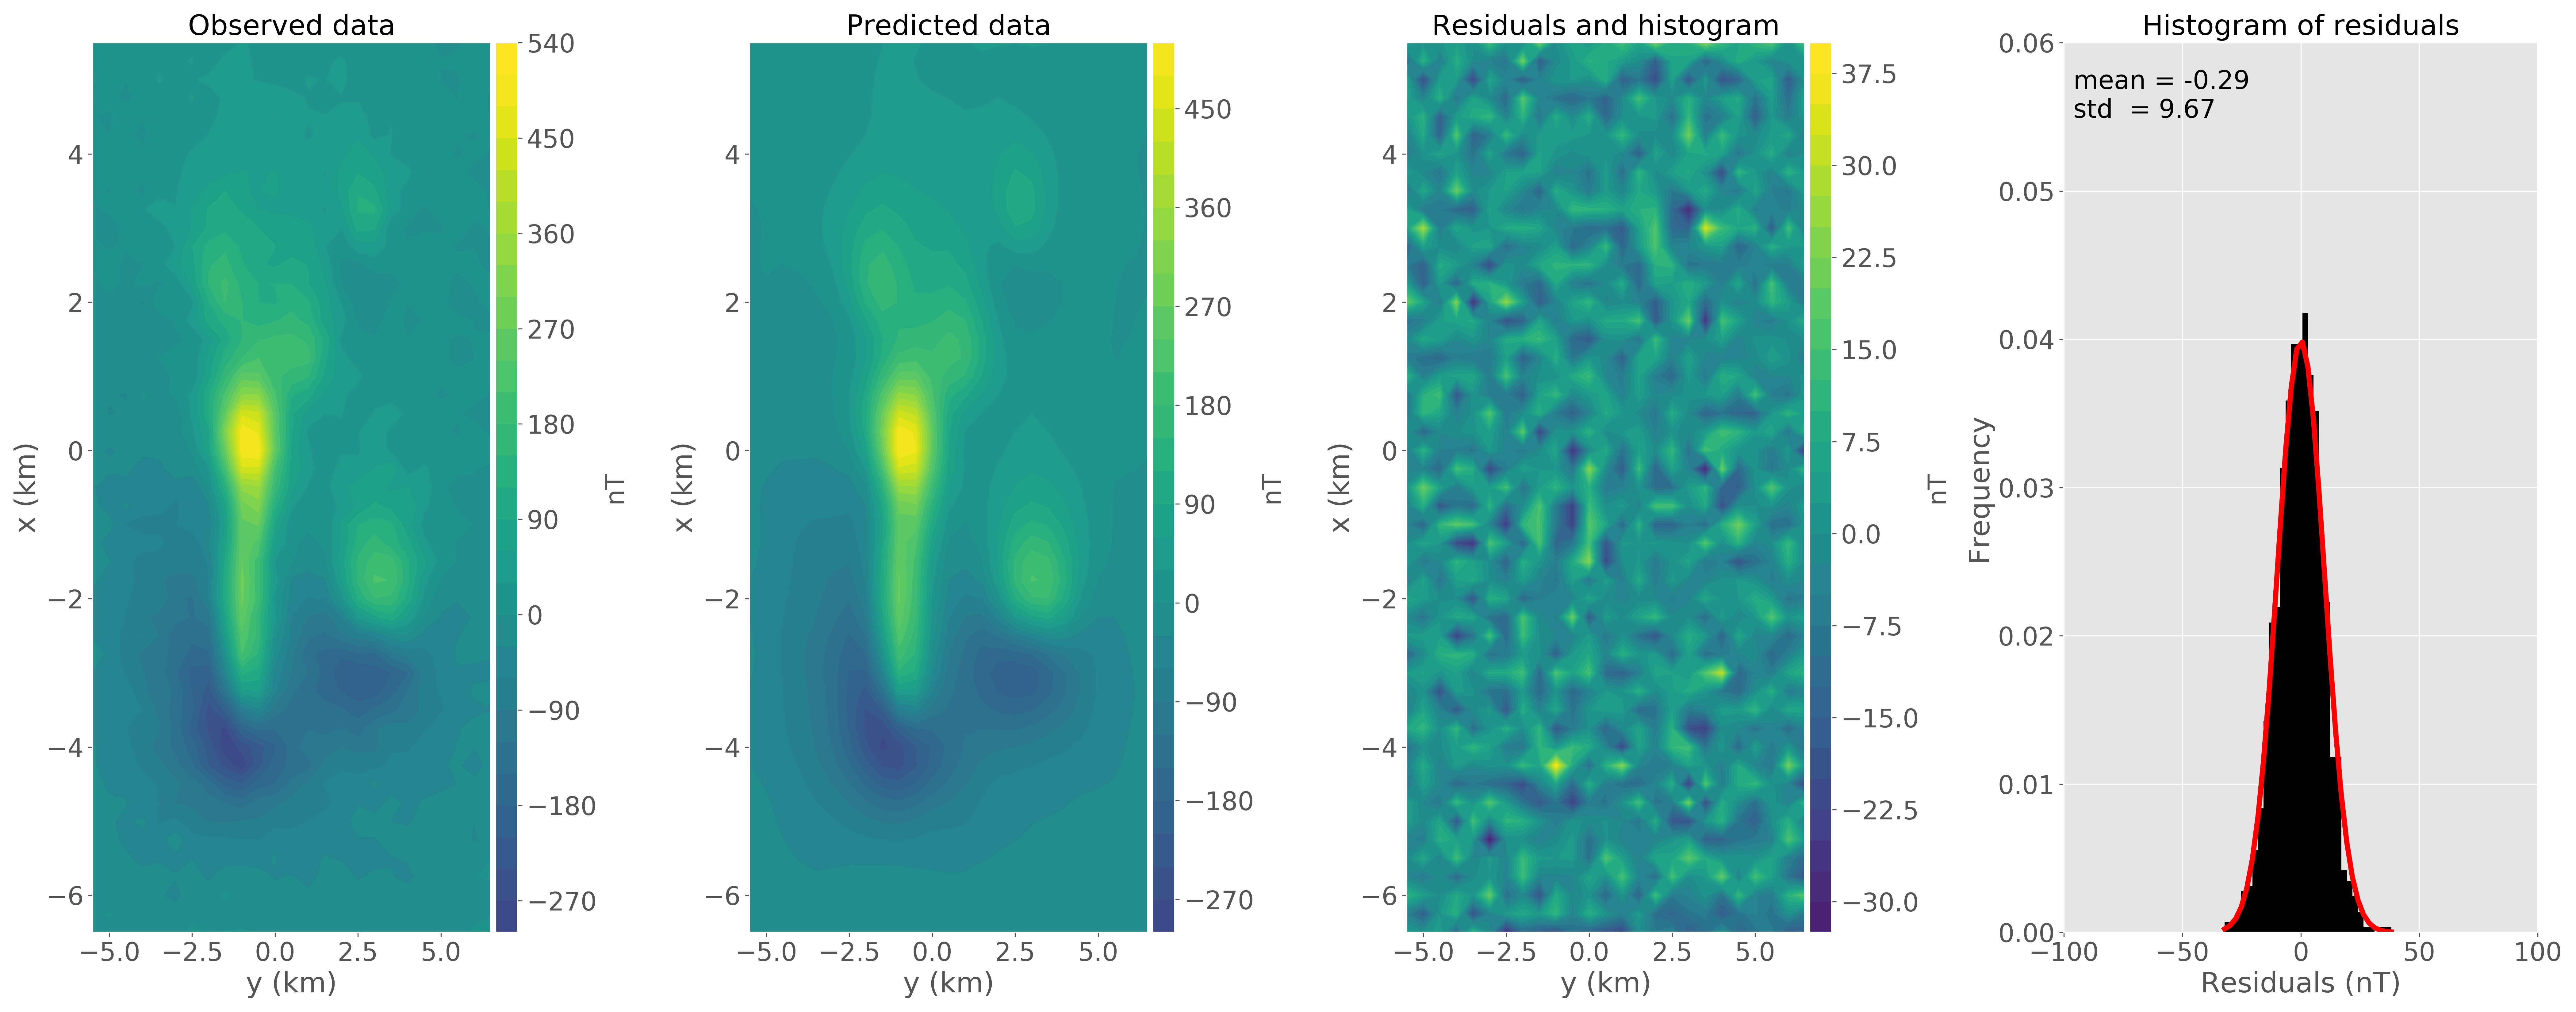
\includegraphics[width=1.1\textwidth]{Fig/eqlayer/unidir_test/data_fitting_LM_NNLS_magRM.png}
	\caption{Aplicação a dados sintéticos para múltiplas fontes de mesma direção de magnetização. (a) Anomalia de campo total observada. (b) Dados preditos produzido pela camada equivalente. (c) Diferença entre os dados mostrados nos gráficos a e b. (d) Histograma dos resíduos.}
	\label{fig:data_fitting_1}
\end{figure}

\begin{figure}
	\centering
	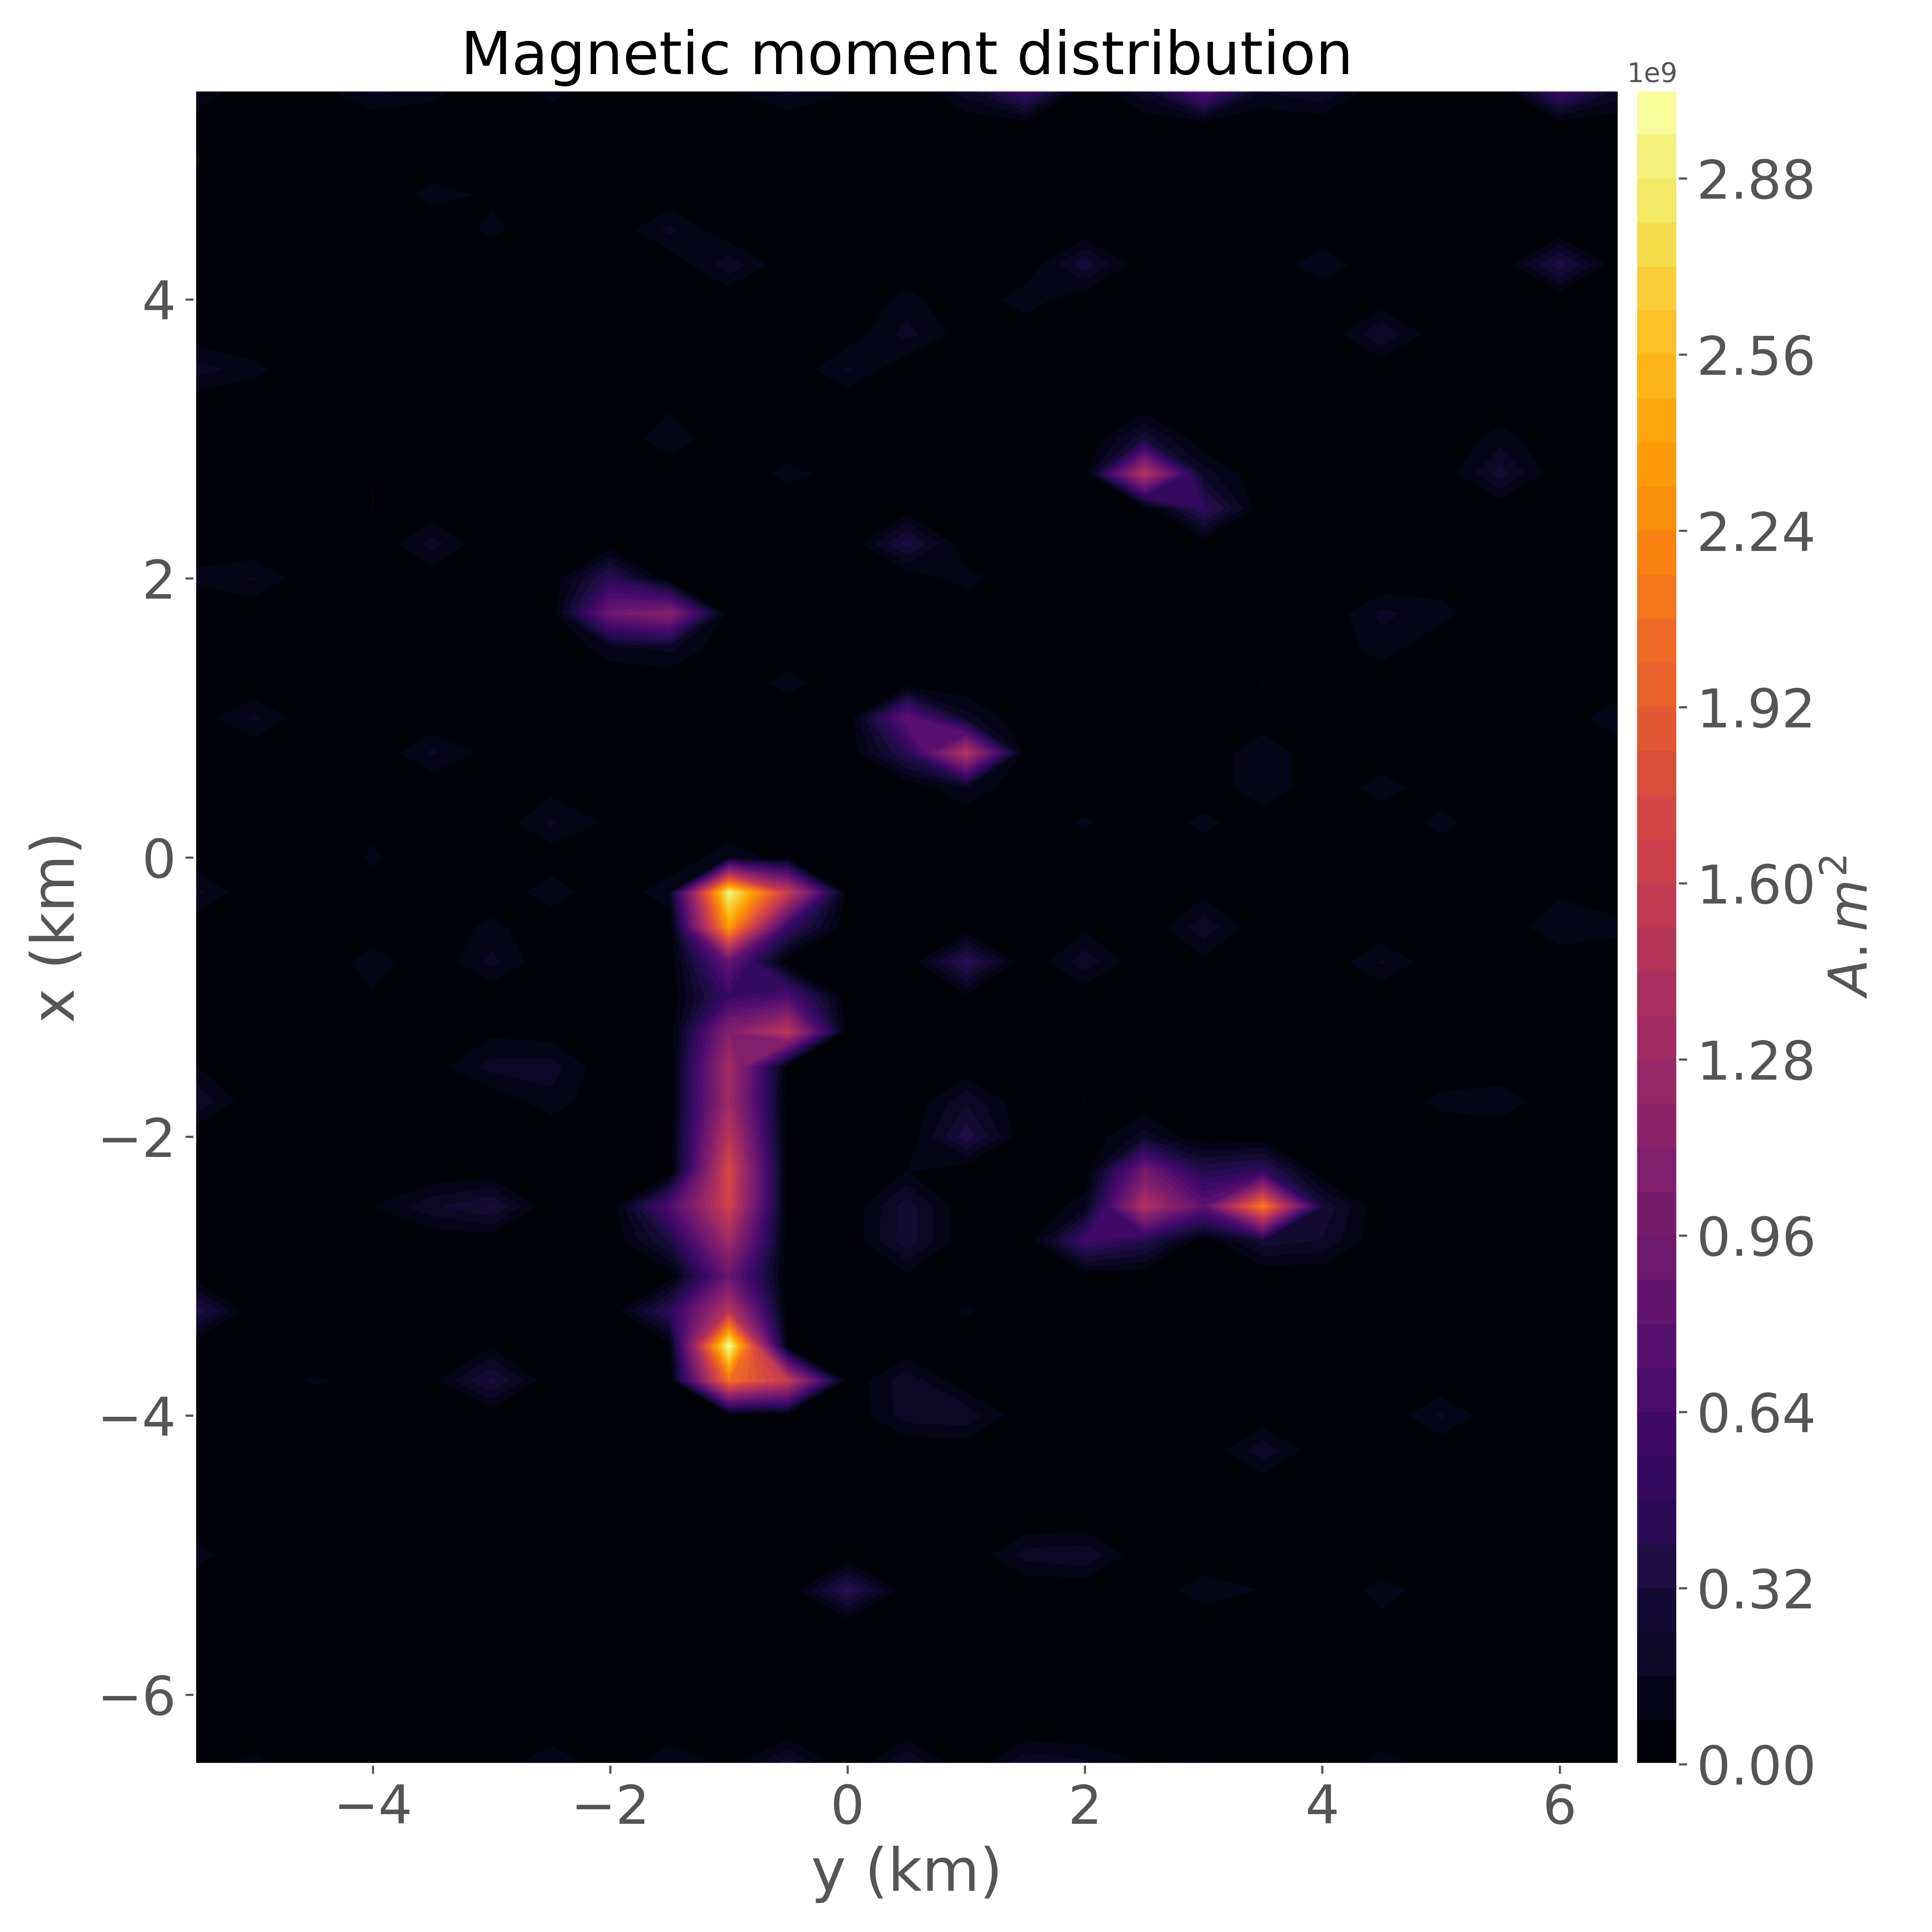
\includegraphics[width=.9\textwidth]{Fig/eqlayer/unidir_test/magnetic_moment_positive_LM_NNLS_magRM.png}
	\caption{Distribuição de momentos magnéticos positiva para a aplicação a dados sintéticos para múltiplas fontes de mesma direção de magnetização.}
	\label{fig:dist_momentos_pos_1}
\end{figure}

\begin{figure}
	\centering
	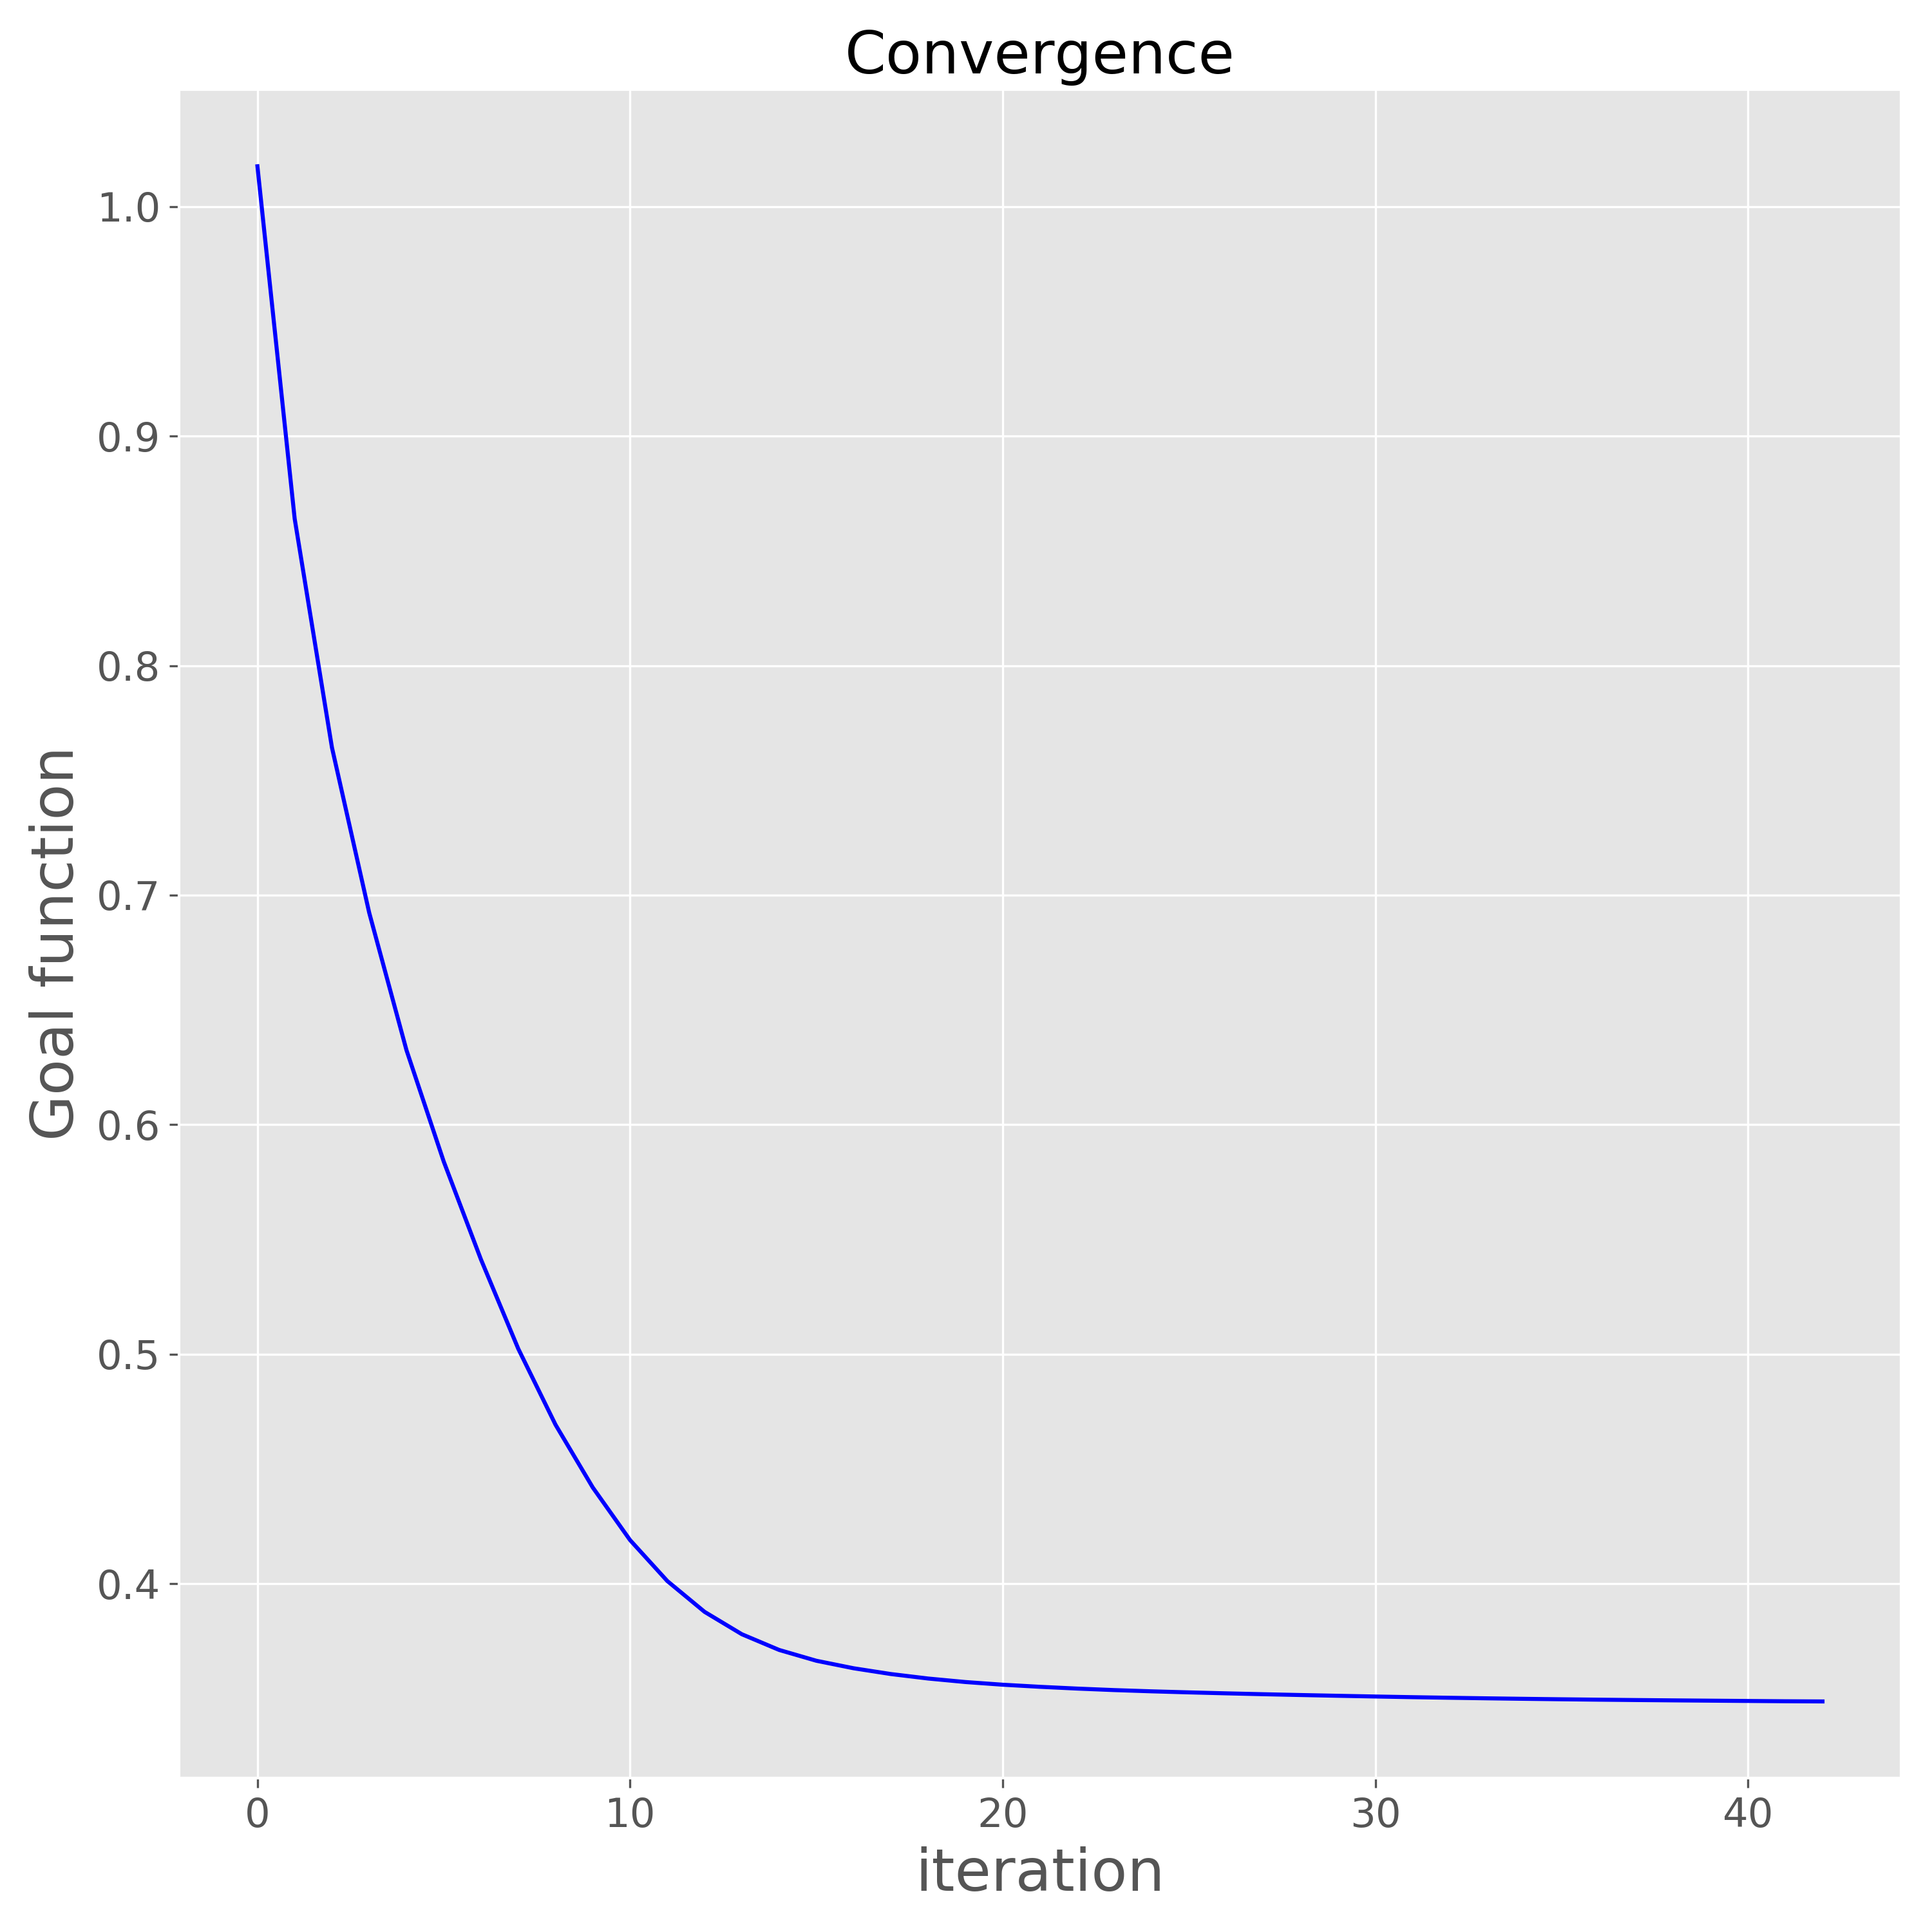
\includegraphics[width=.9\textwidth]{Fig/eqlayer/unidir_test/convergence_LM_NNLS_magRM.png}
	\caption{Valor da função objetivo ao longo das iterações (equação \ref{eq:positivity_goal_function}a) mostrando a convergência do algoritmo.}
	\label{fig:convergence_1}
\end{figure}

\begin{figure}
	\centering
	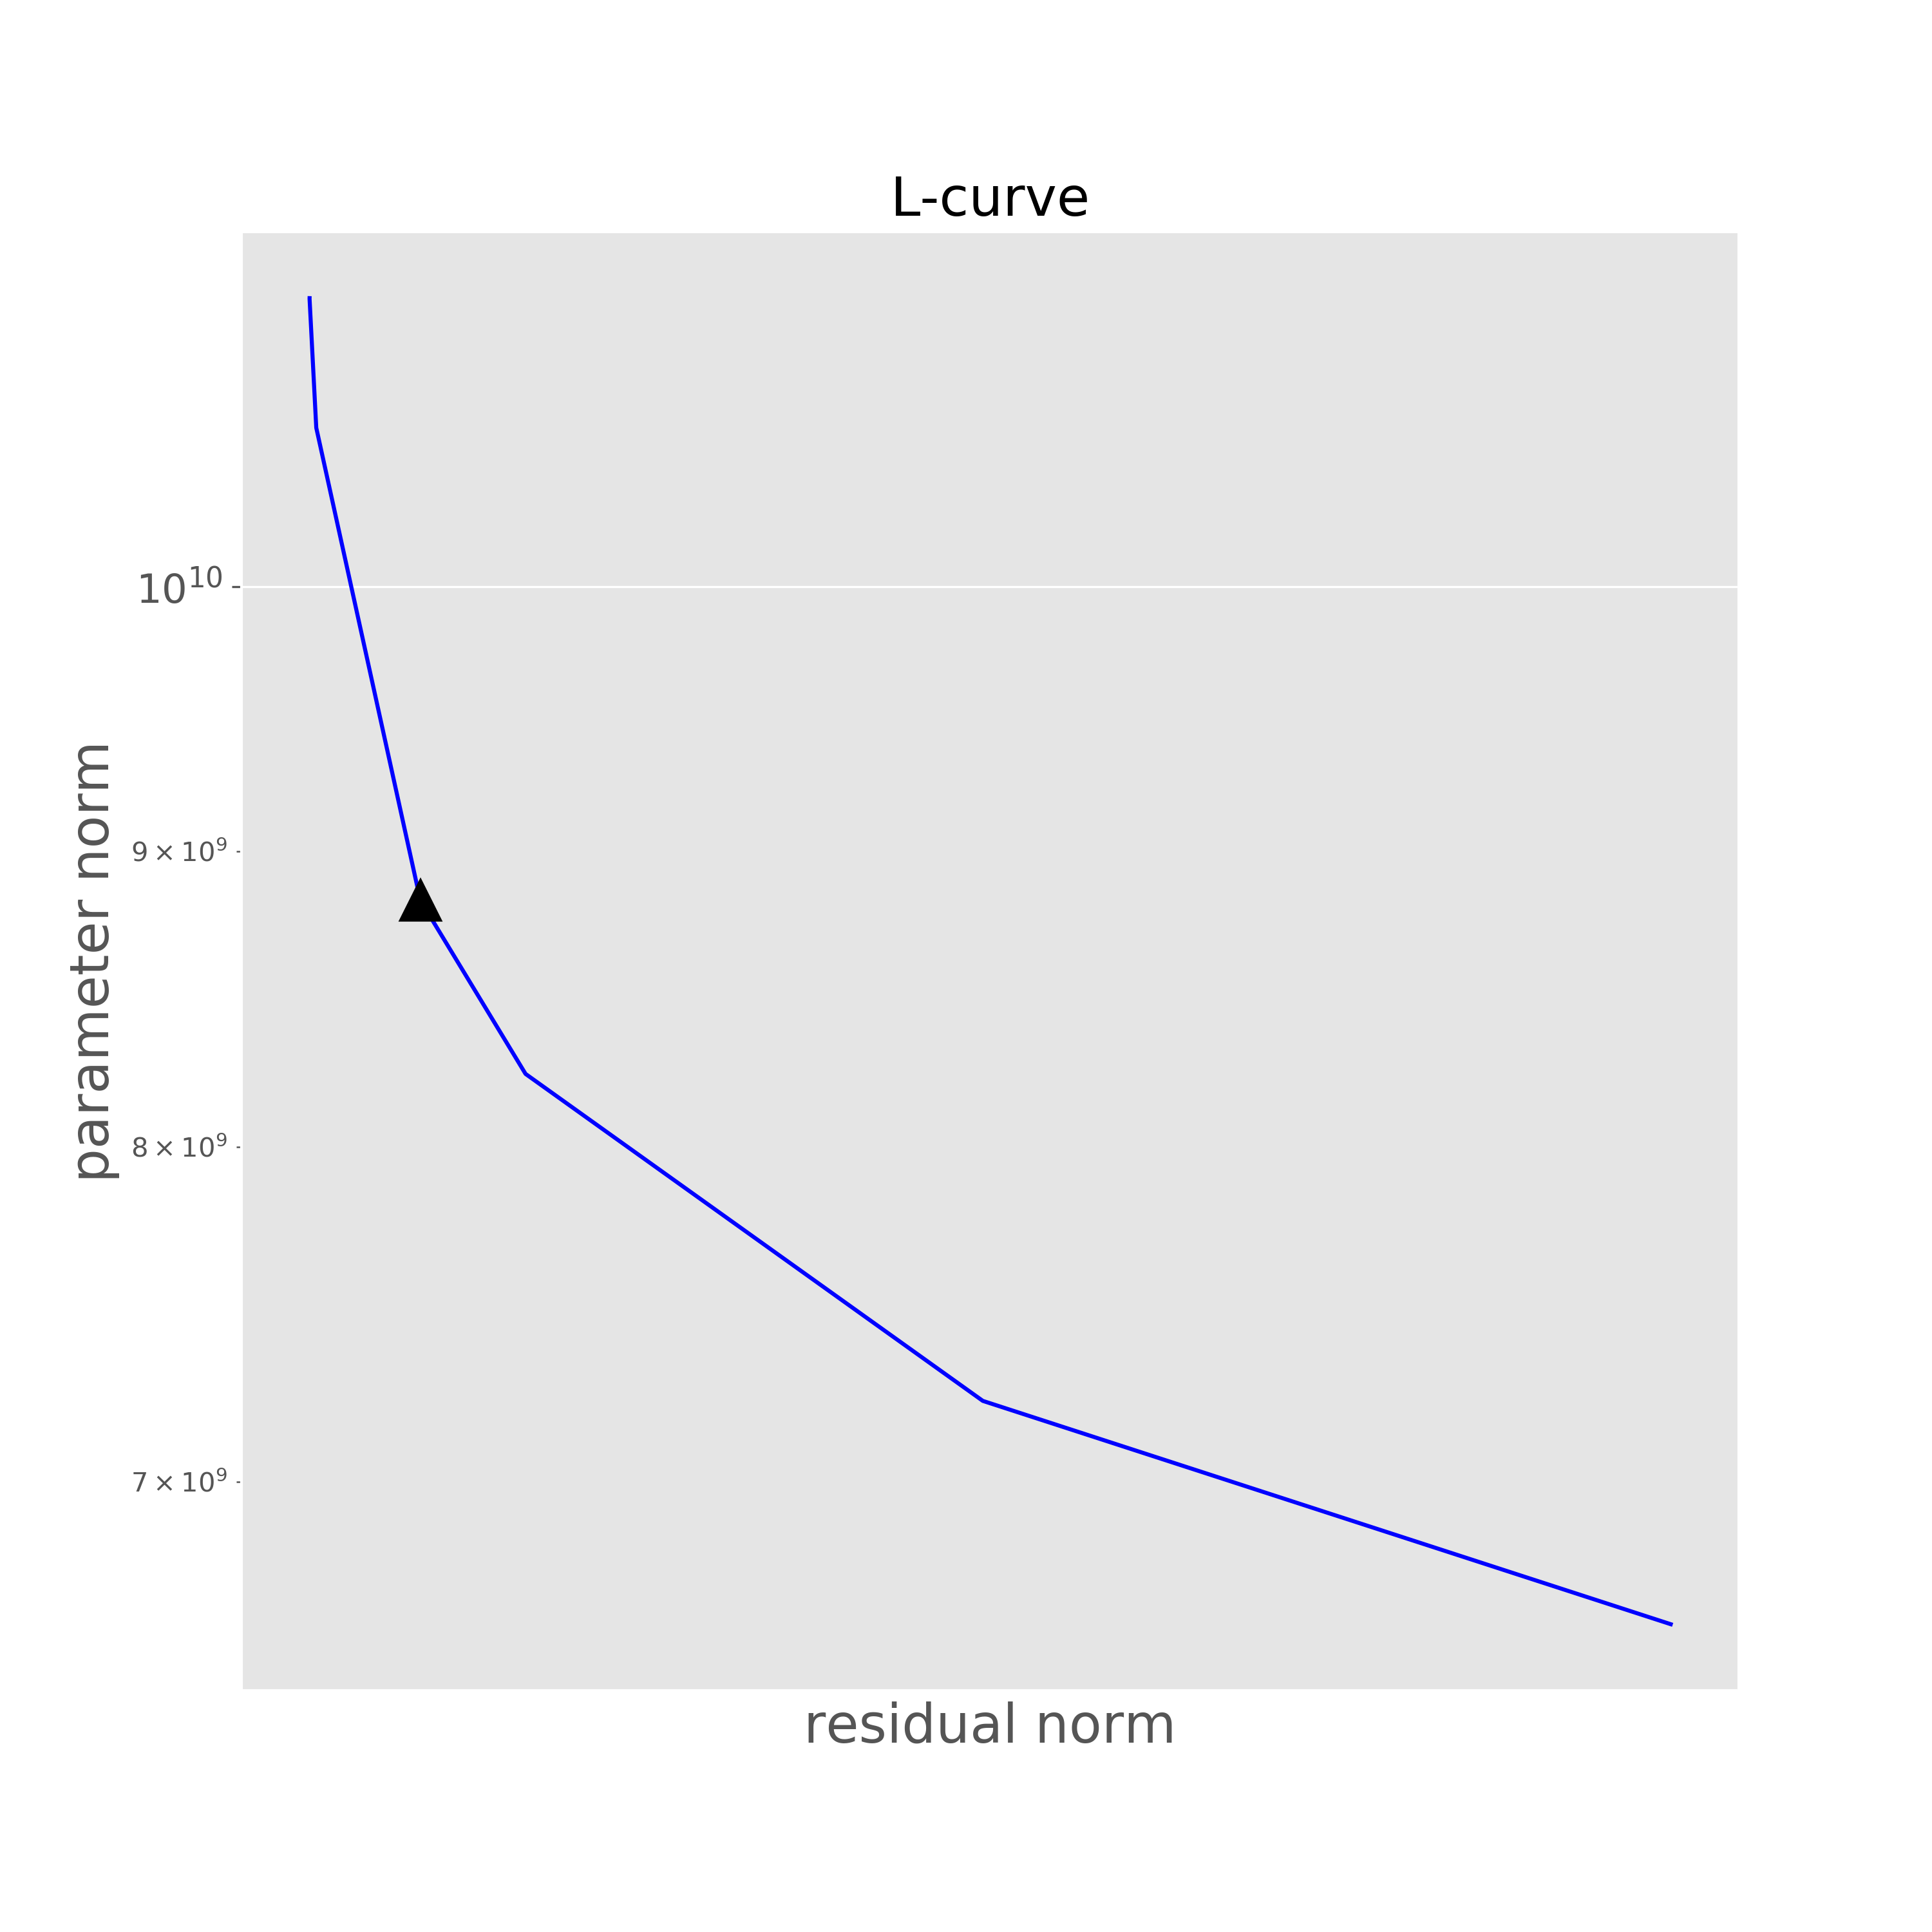
\includegraphics[width=.9\textwidth]{Fig/eqlayer/unidir_test/Lcurve_RM.png}
	\caption{Gráfico da curva-L mostrando a escolha do parâmetro de regularização $\mu$ (equação \ref{eq:positivity_goal_function}a). O triângulo em preto indica o ponto no qual foi escolhido o parâmetro igual a $350000$.}
	\label{fig:lcurve_1}
\end{figure}


\section{Magnetização unidirecional com fonte rasa}

Testamos a performance do método quando existe uma fonte rasa. O modelo é similar ao anterior com exceção do prisma menor, cujo topo é localizado a uma profundidade de $150$ m enquanto seu volume é mantido o mesmo. A intensidade de magnetização deste prisma raso é igual a $1,5$ A/m. A direção de magnetização de todas as fontes é $-25^\circ$ de inclinação e $30^\circ$ graus para a declinação. Os dados sintéticos são mostrados na figura \ref{fig:data_fitting_2}a.

A figura \ref{fig:data_fitting_2}b mostra a anomalia de campo total predita produzida pela camada equivalente. A figura \ref{fig:data_fitting_2}c mostra o mapa dos resíduos definido como a diferença entre a anomalia de campo total observada (Figura \ref{fig:data_fitting_2}a) e a anomalia de campo total predita (Figura \ref{fig:data_fitting_2}b). Os resíduos aparecem com uma distribuição normal de média $-0,42$ nT e desvio padrão de $10,67$ nT como mostra a figura \ref{fig:data_fitting_2}d. A figura \ref{fig:dist_momentos_pos_2} mostra a distribuição de momentos magnéticos $\bar{\mathbf{p}}$. A convergência do algoritmo é mostrada na figura \ref{fig:convergence_2}. A escolha do parâmetro de regularização $\mu = 3500000$ é mostrada na figura \ref{fig:lcurve_2}. Apesar do grande resíduo acima da fonte rasa, consideramos que a metodologia produziu uma confiável estimativa para a direção de magnetização $\bar{\mathbf{q}}$, que possui inclinação $-28,7^\circ$ e declination $31,7^\circ$. A direção de magnetização estimada é próxima a direção verdadeira e a distribuição de momentos magnéticos produziu um ajuste aceitável dos dados. 

%%% Figuras teste 2 
\begin{figure}
	\centering
	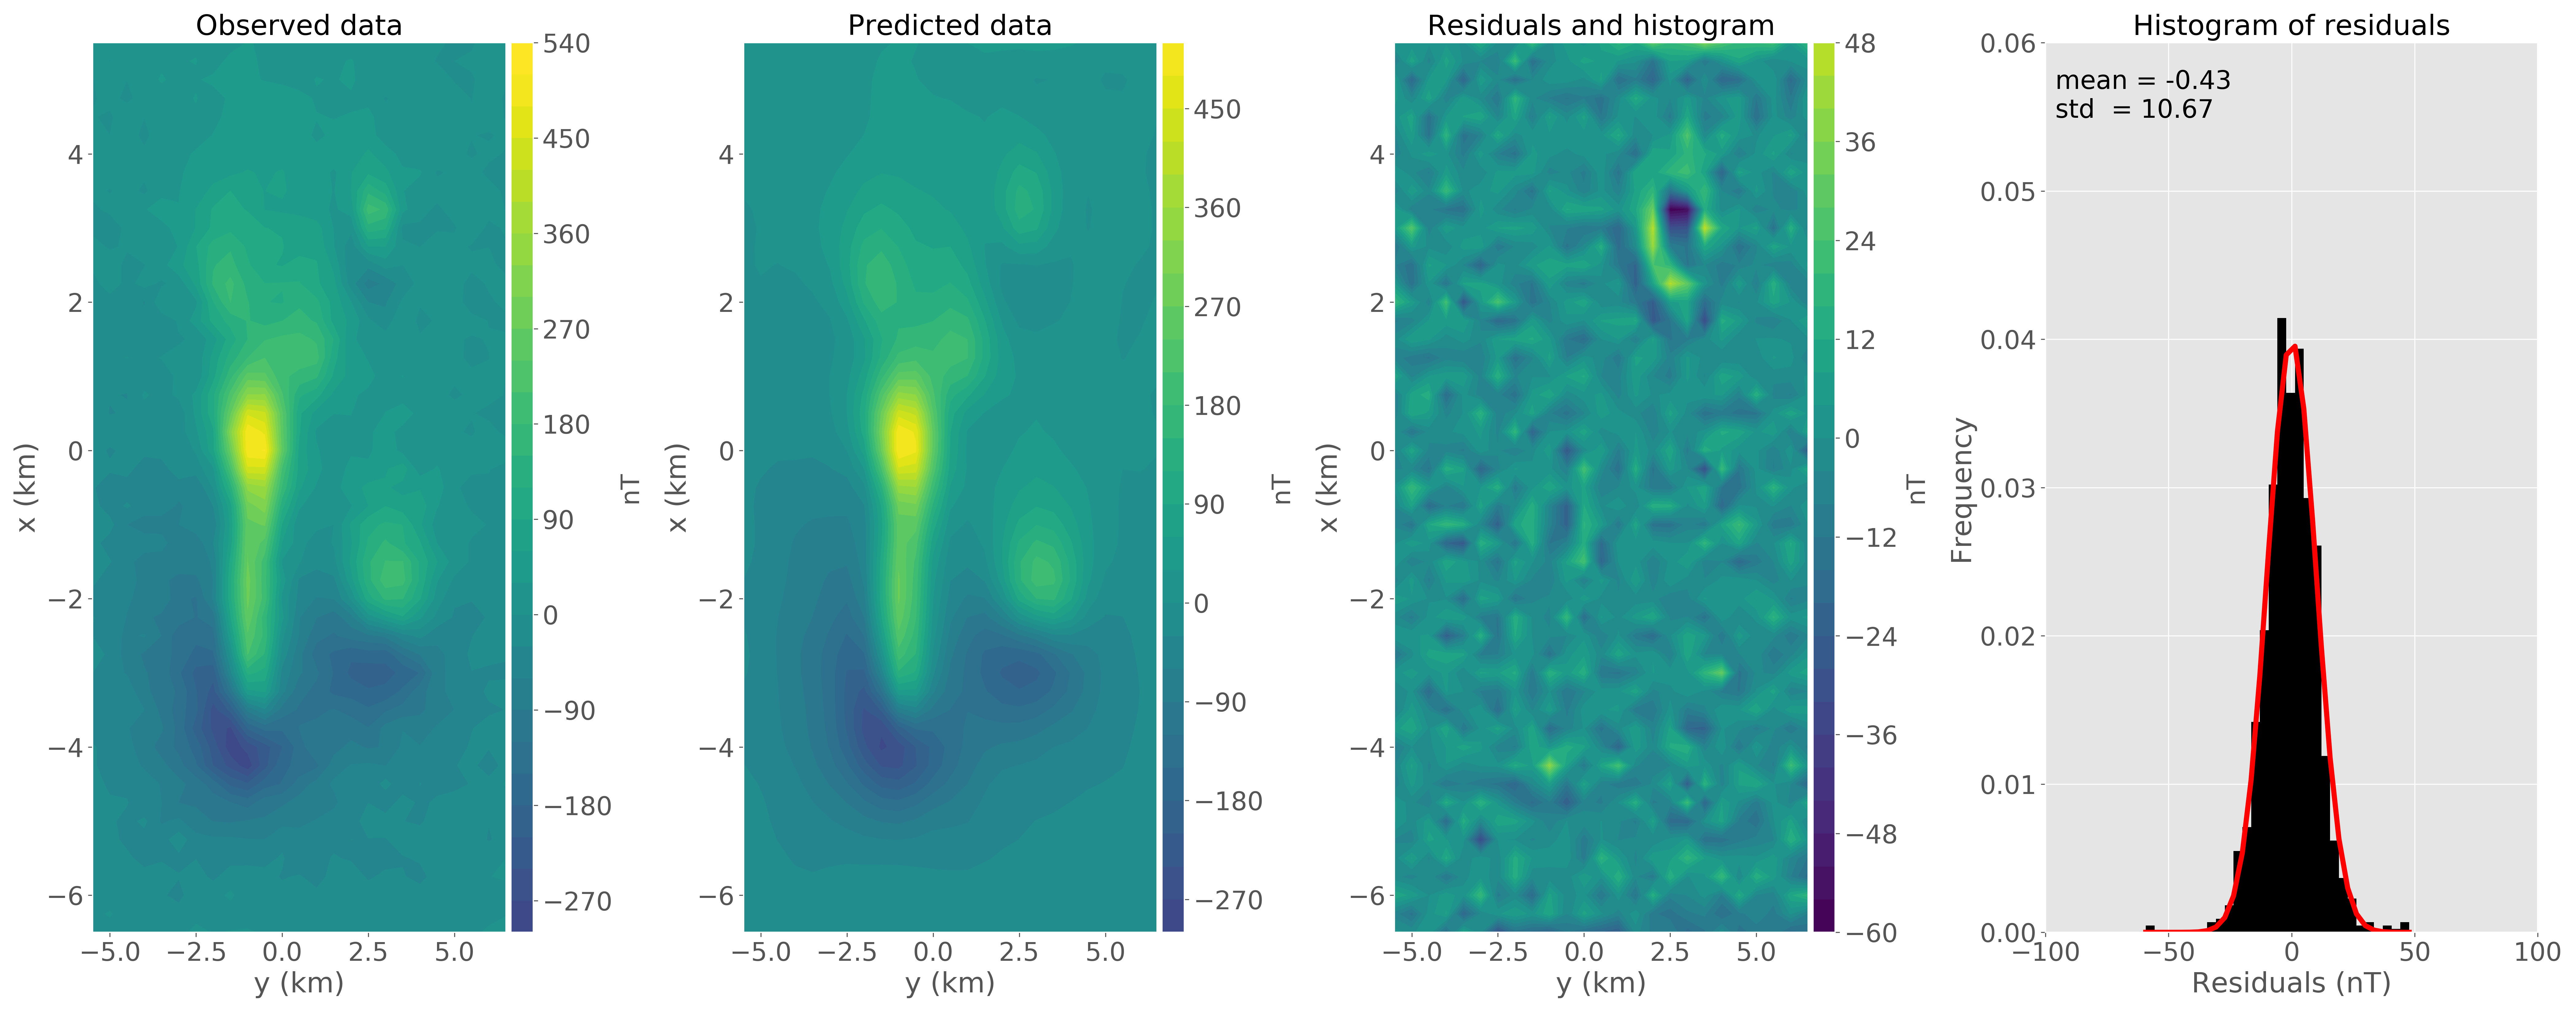
\includegraphics[width=1.1\textwidth]{Fig/eqlayer/unidir_shallow_test/data_fitting_LM_NNLS_magRM.png}
	\caption{Aplicação a dados sintéticos para múltiplos corpos com fonte rasa e mesma direção de magnetização. (a) Anomalia de campo total observada. (b) Dados preditos produzido pela camada equivalente. (c) Diferença entre os dados mostrados nos gráficos a e b. (d) Histograma dos resíduos.}
	\label{fig:data_fitting_2}
\end{figure}

\begin{figure}
	\centering
	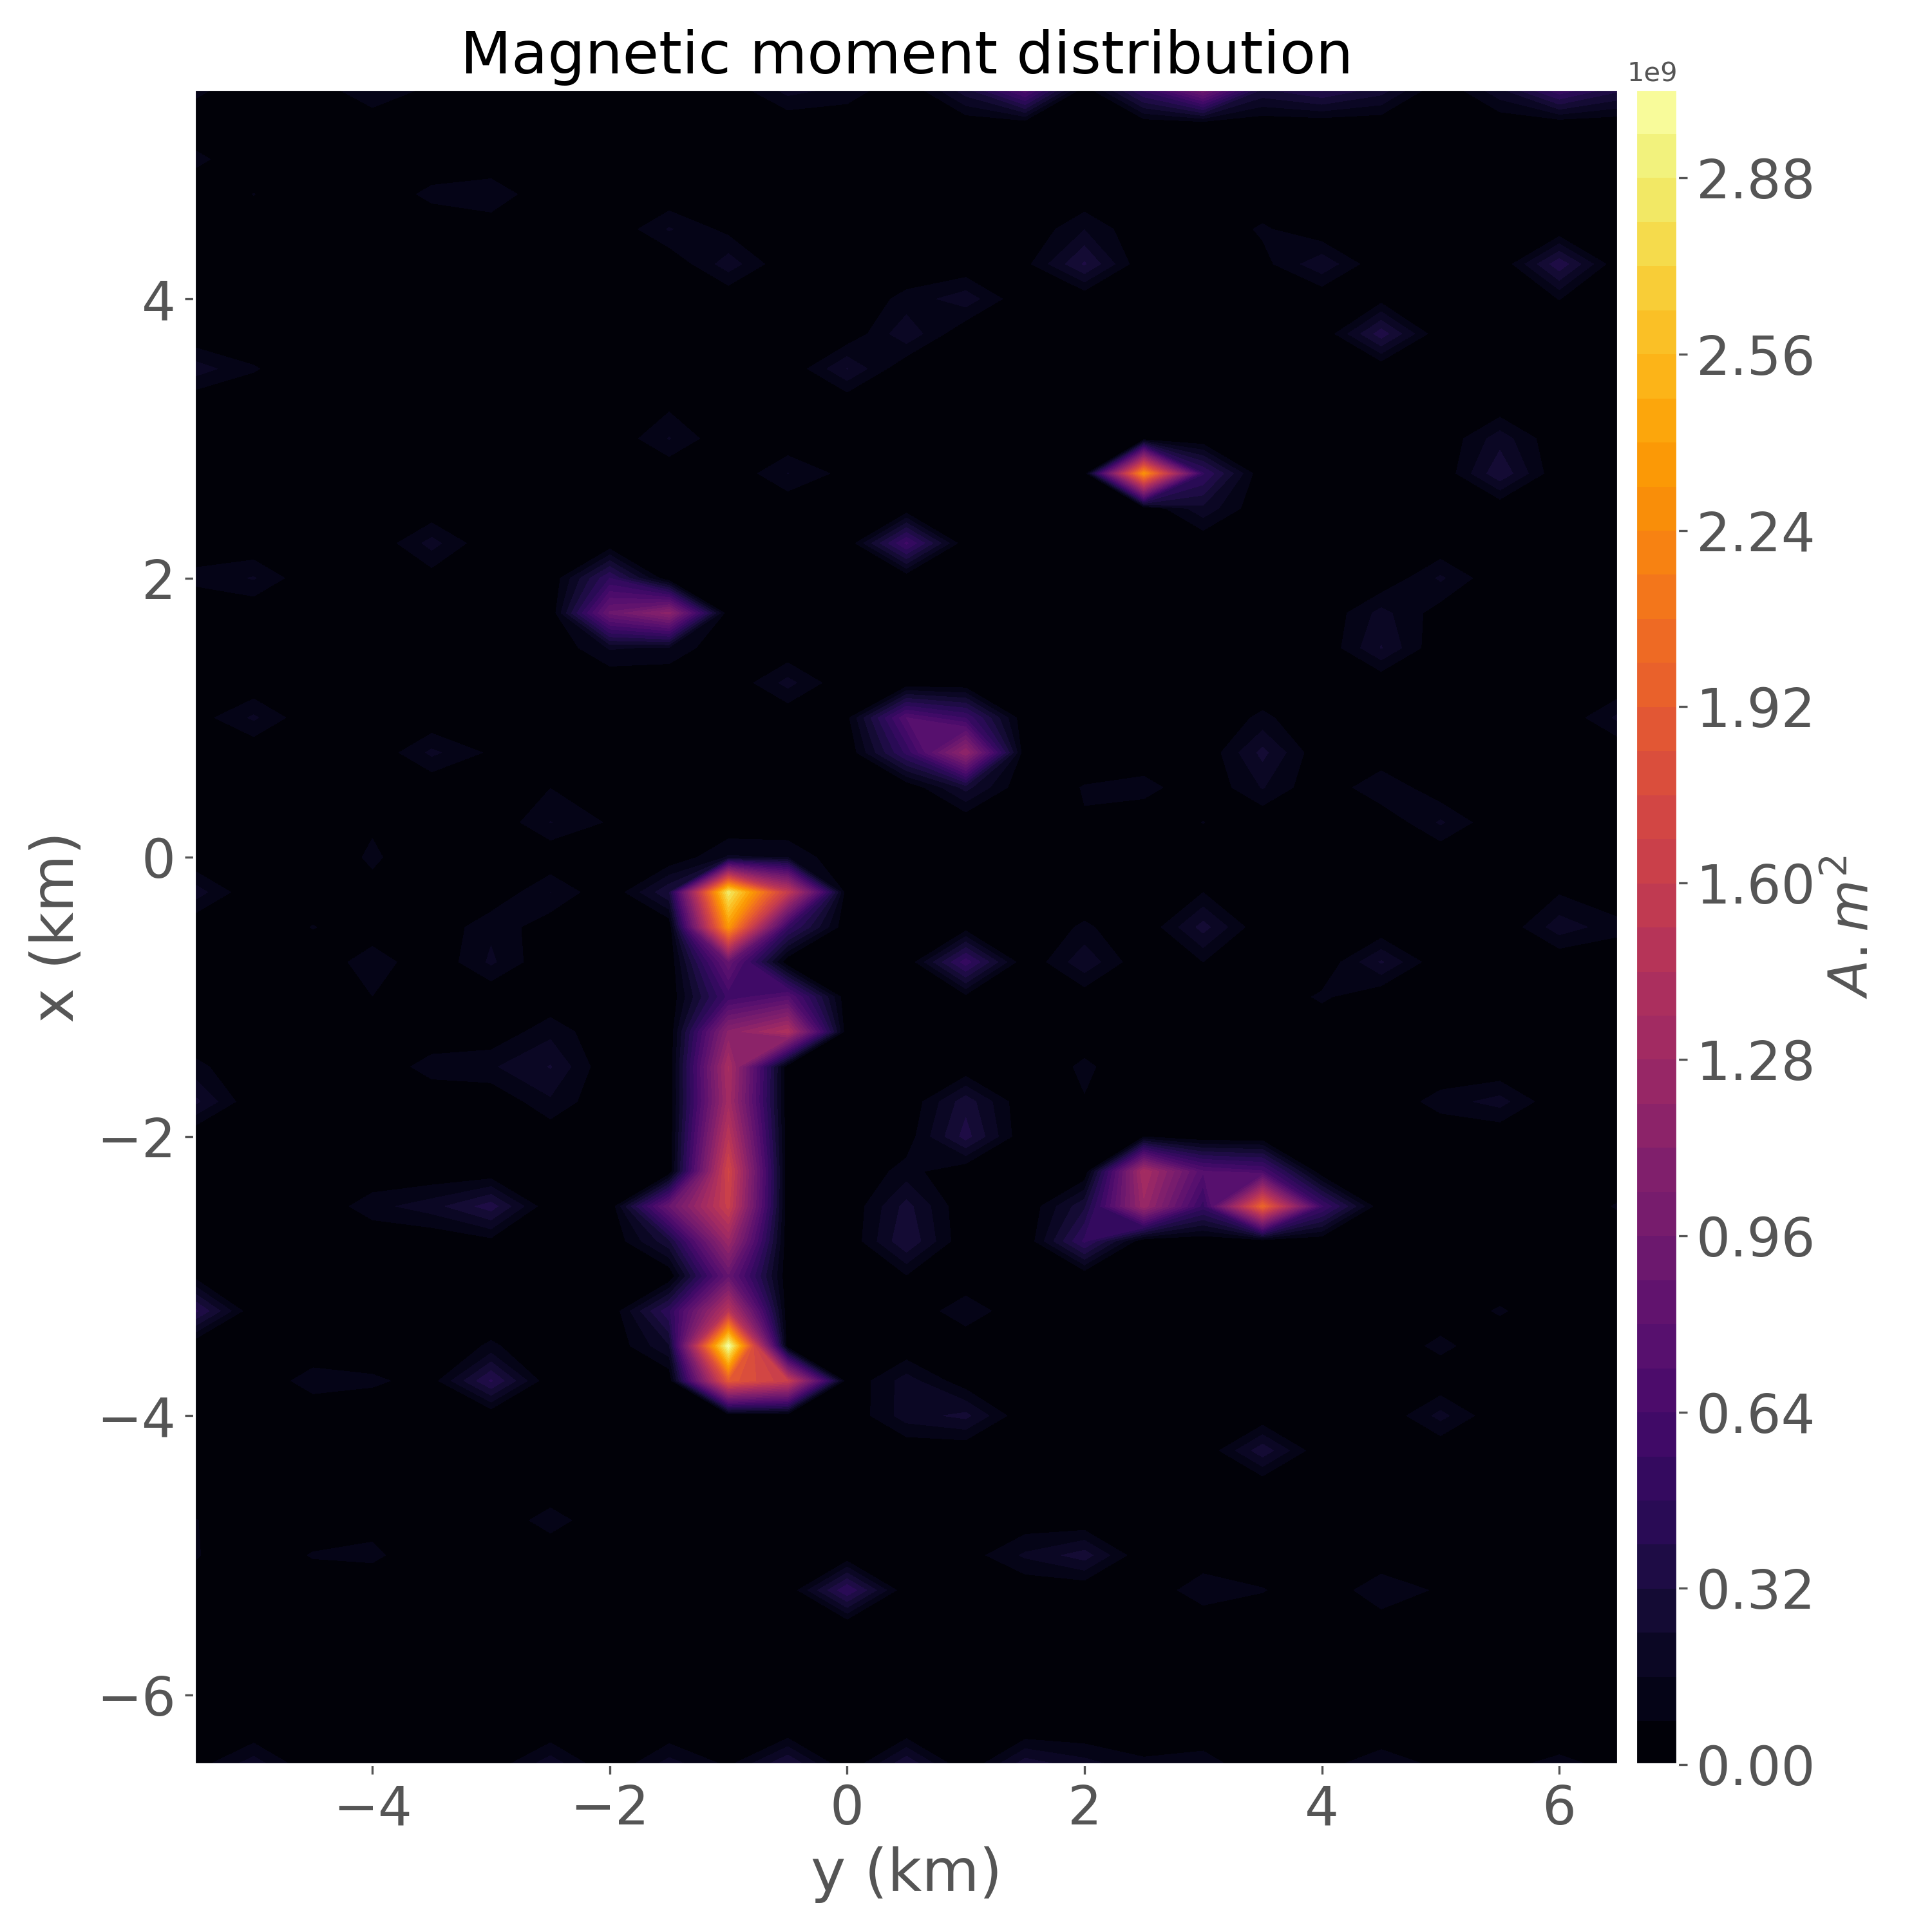
\includegraphics[width=.9\textwidth]{Fig/eqlayer/unidir_shallow_test/magnetic_moment_positive_LM_NNLS_magRM.png}
	\caption{Distribuição de momentos magnéticos positiva para a aplicação a dados sintéticos para múltiplos corpos e fonte rasa com mesma direção de magnetização.}
	\label{fig:dist_momentos_pos_2}
\end{figure}

\begin{figure}
	\centering
	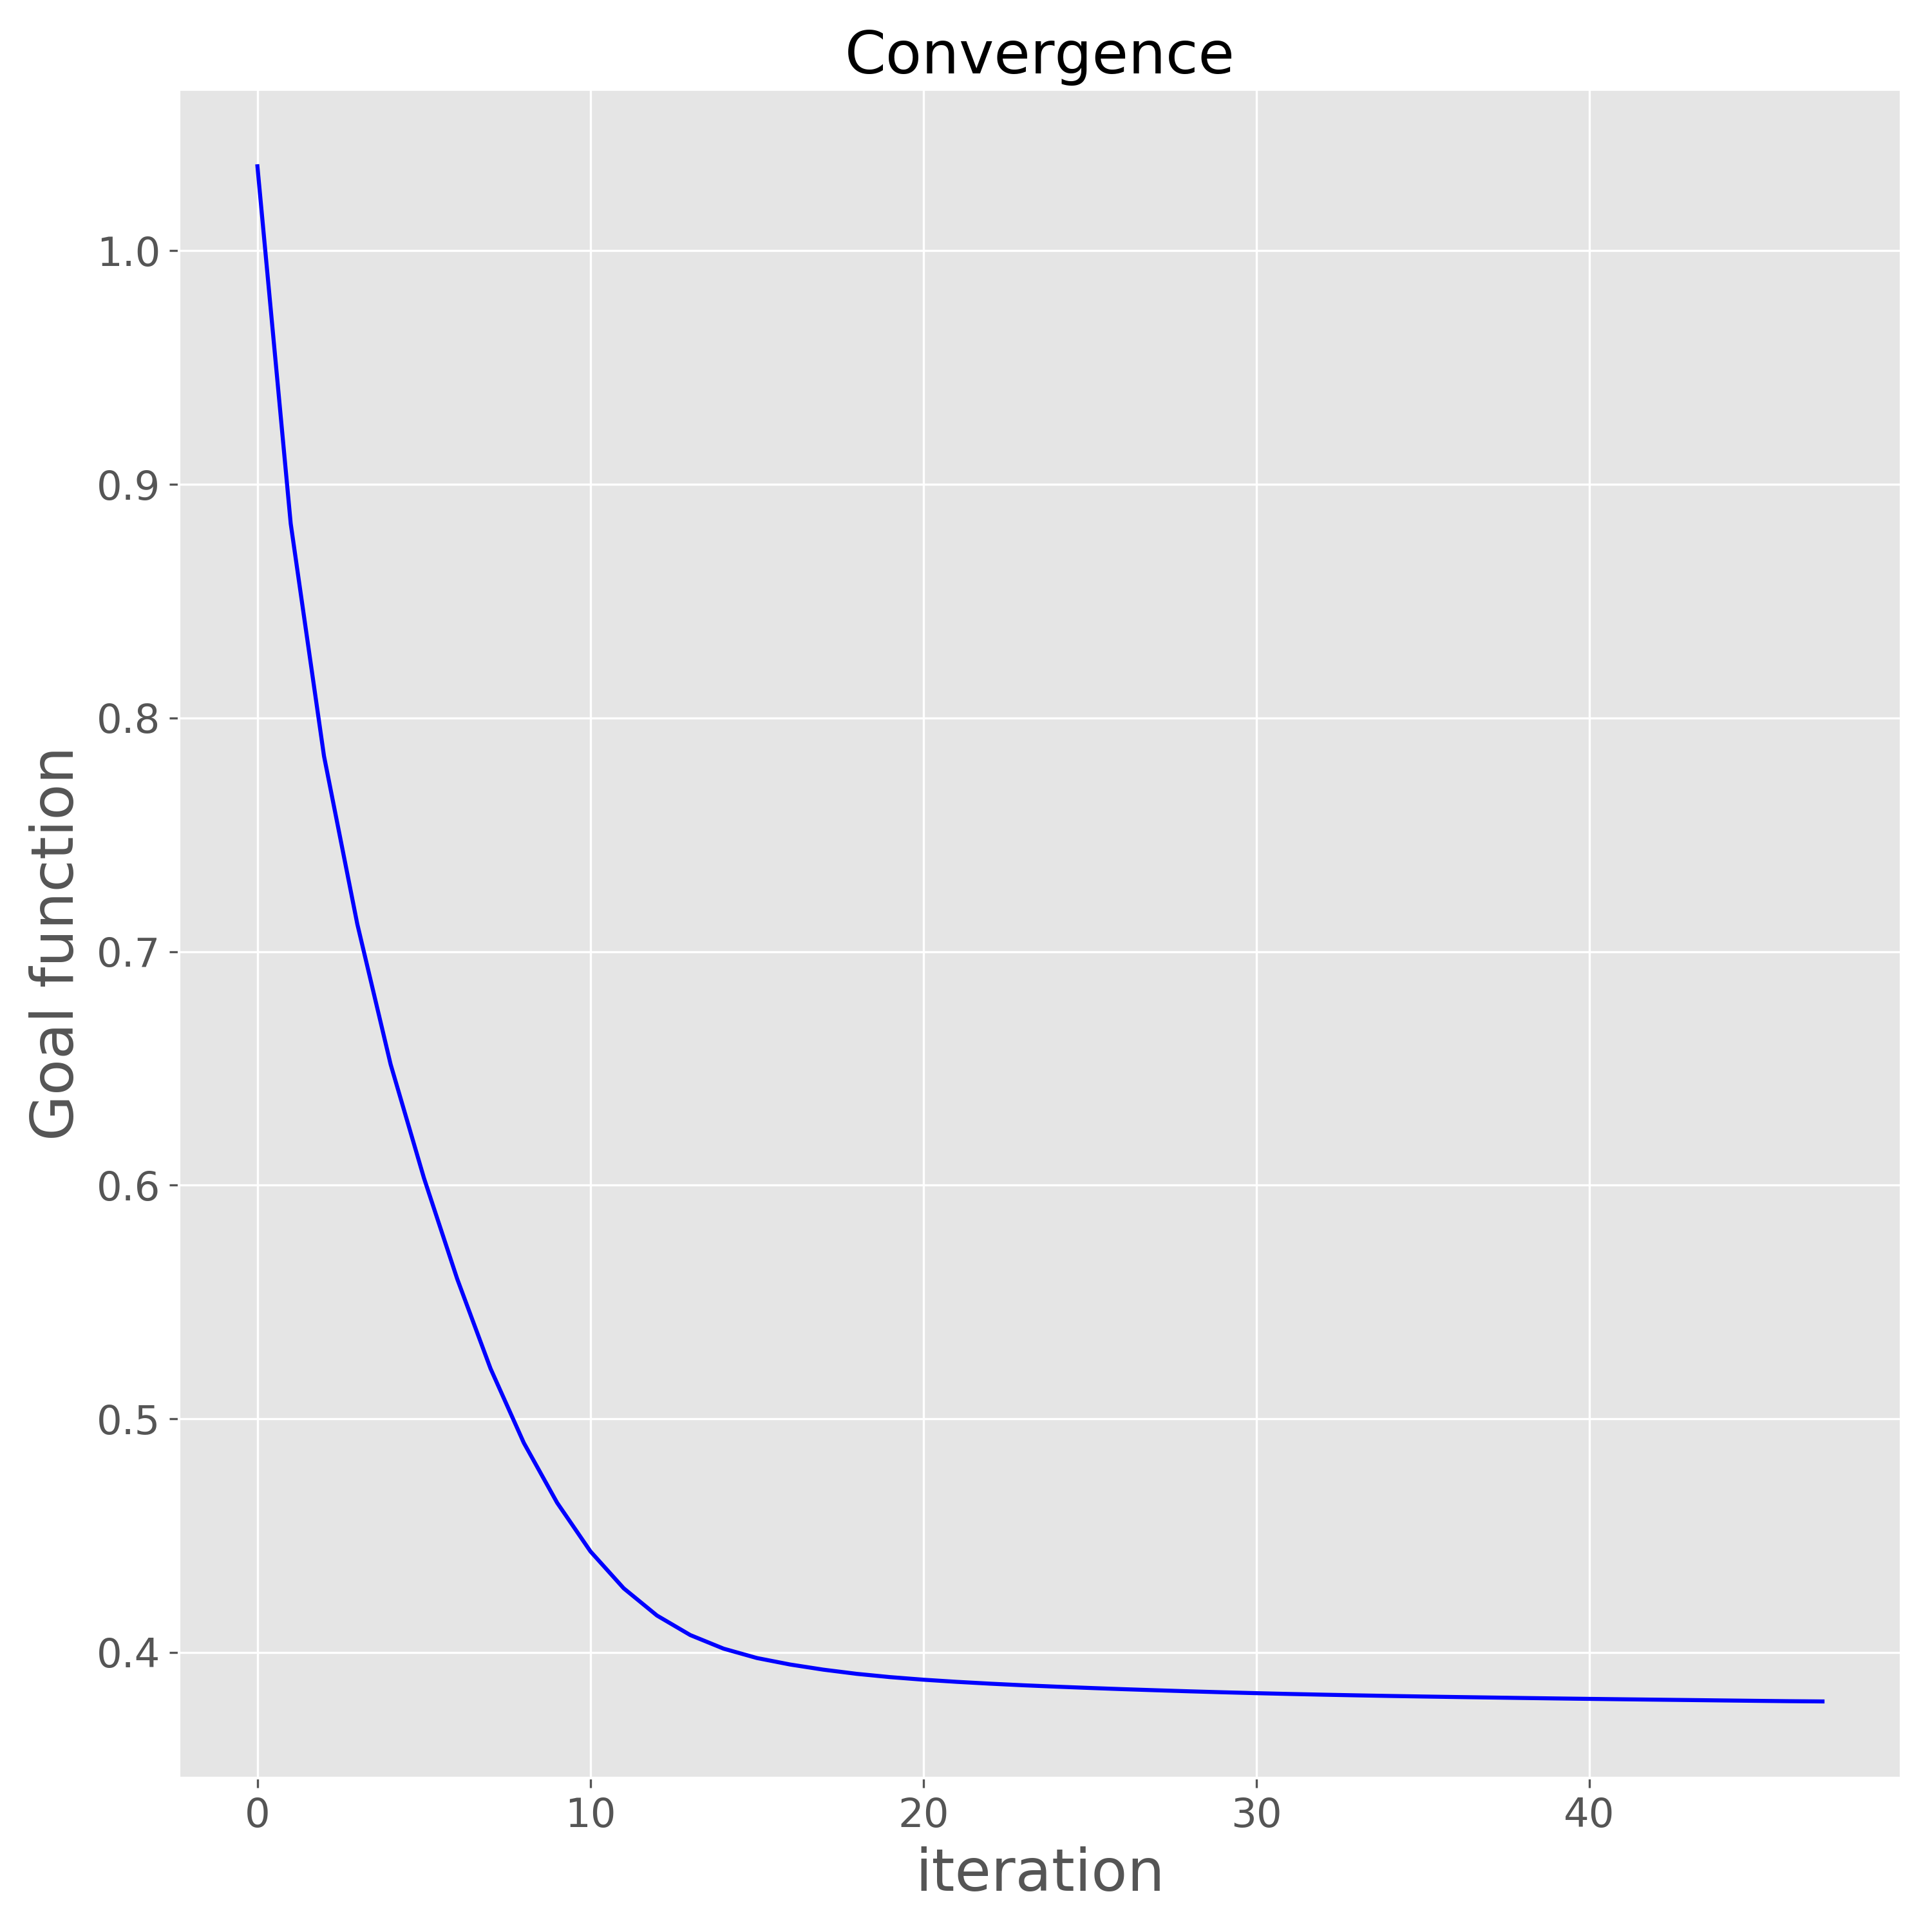
\includegraphics[width=.9\textwidth]{Fig/eqlayer/unidir_shallow_test/convergence_LM_NNLS_magRM.png}
	\caption{Valor da função objetivo ao longo das iterações (equação \ref{eq:positivity_goal_function}a) mostrando a convergência do algoritmo.}
	\label{fig:convergence_2}
\end{figure}

\begin{figure}
	\centering
	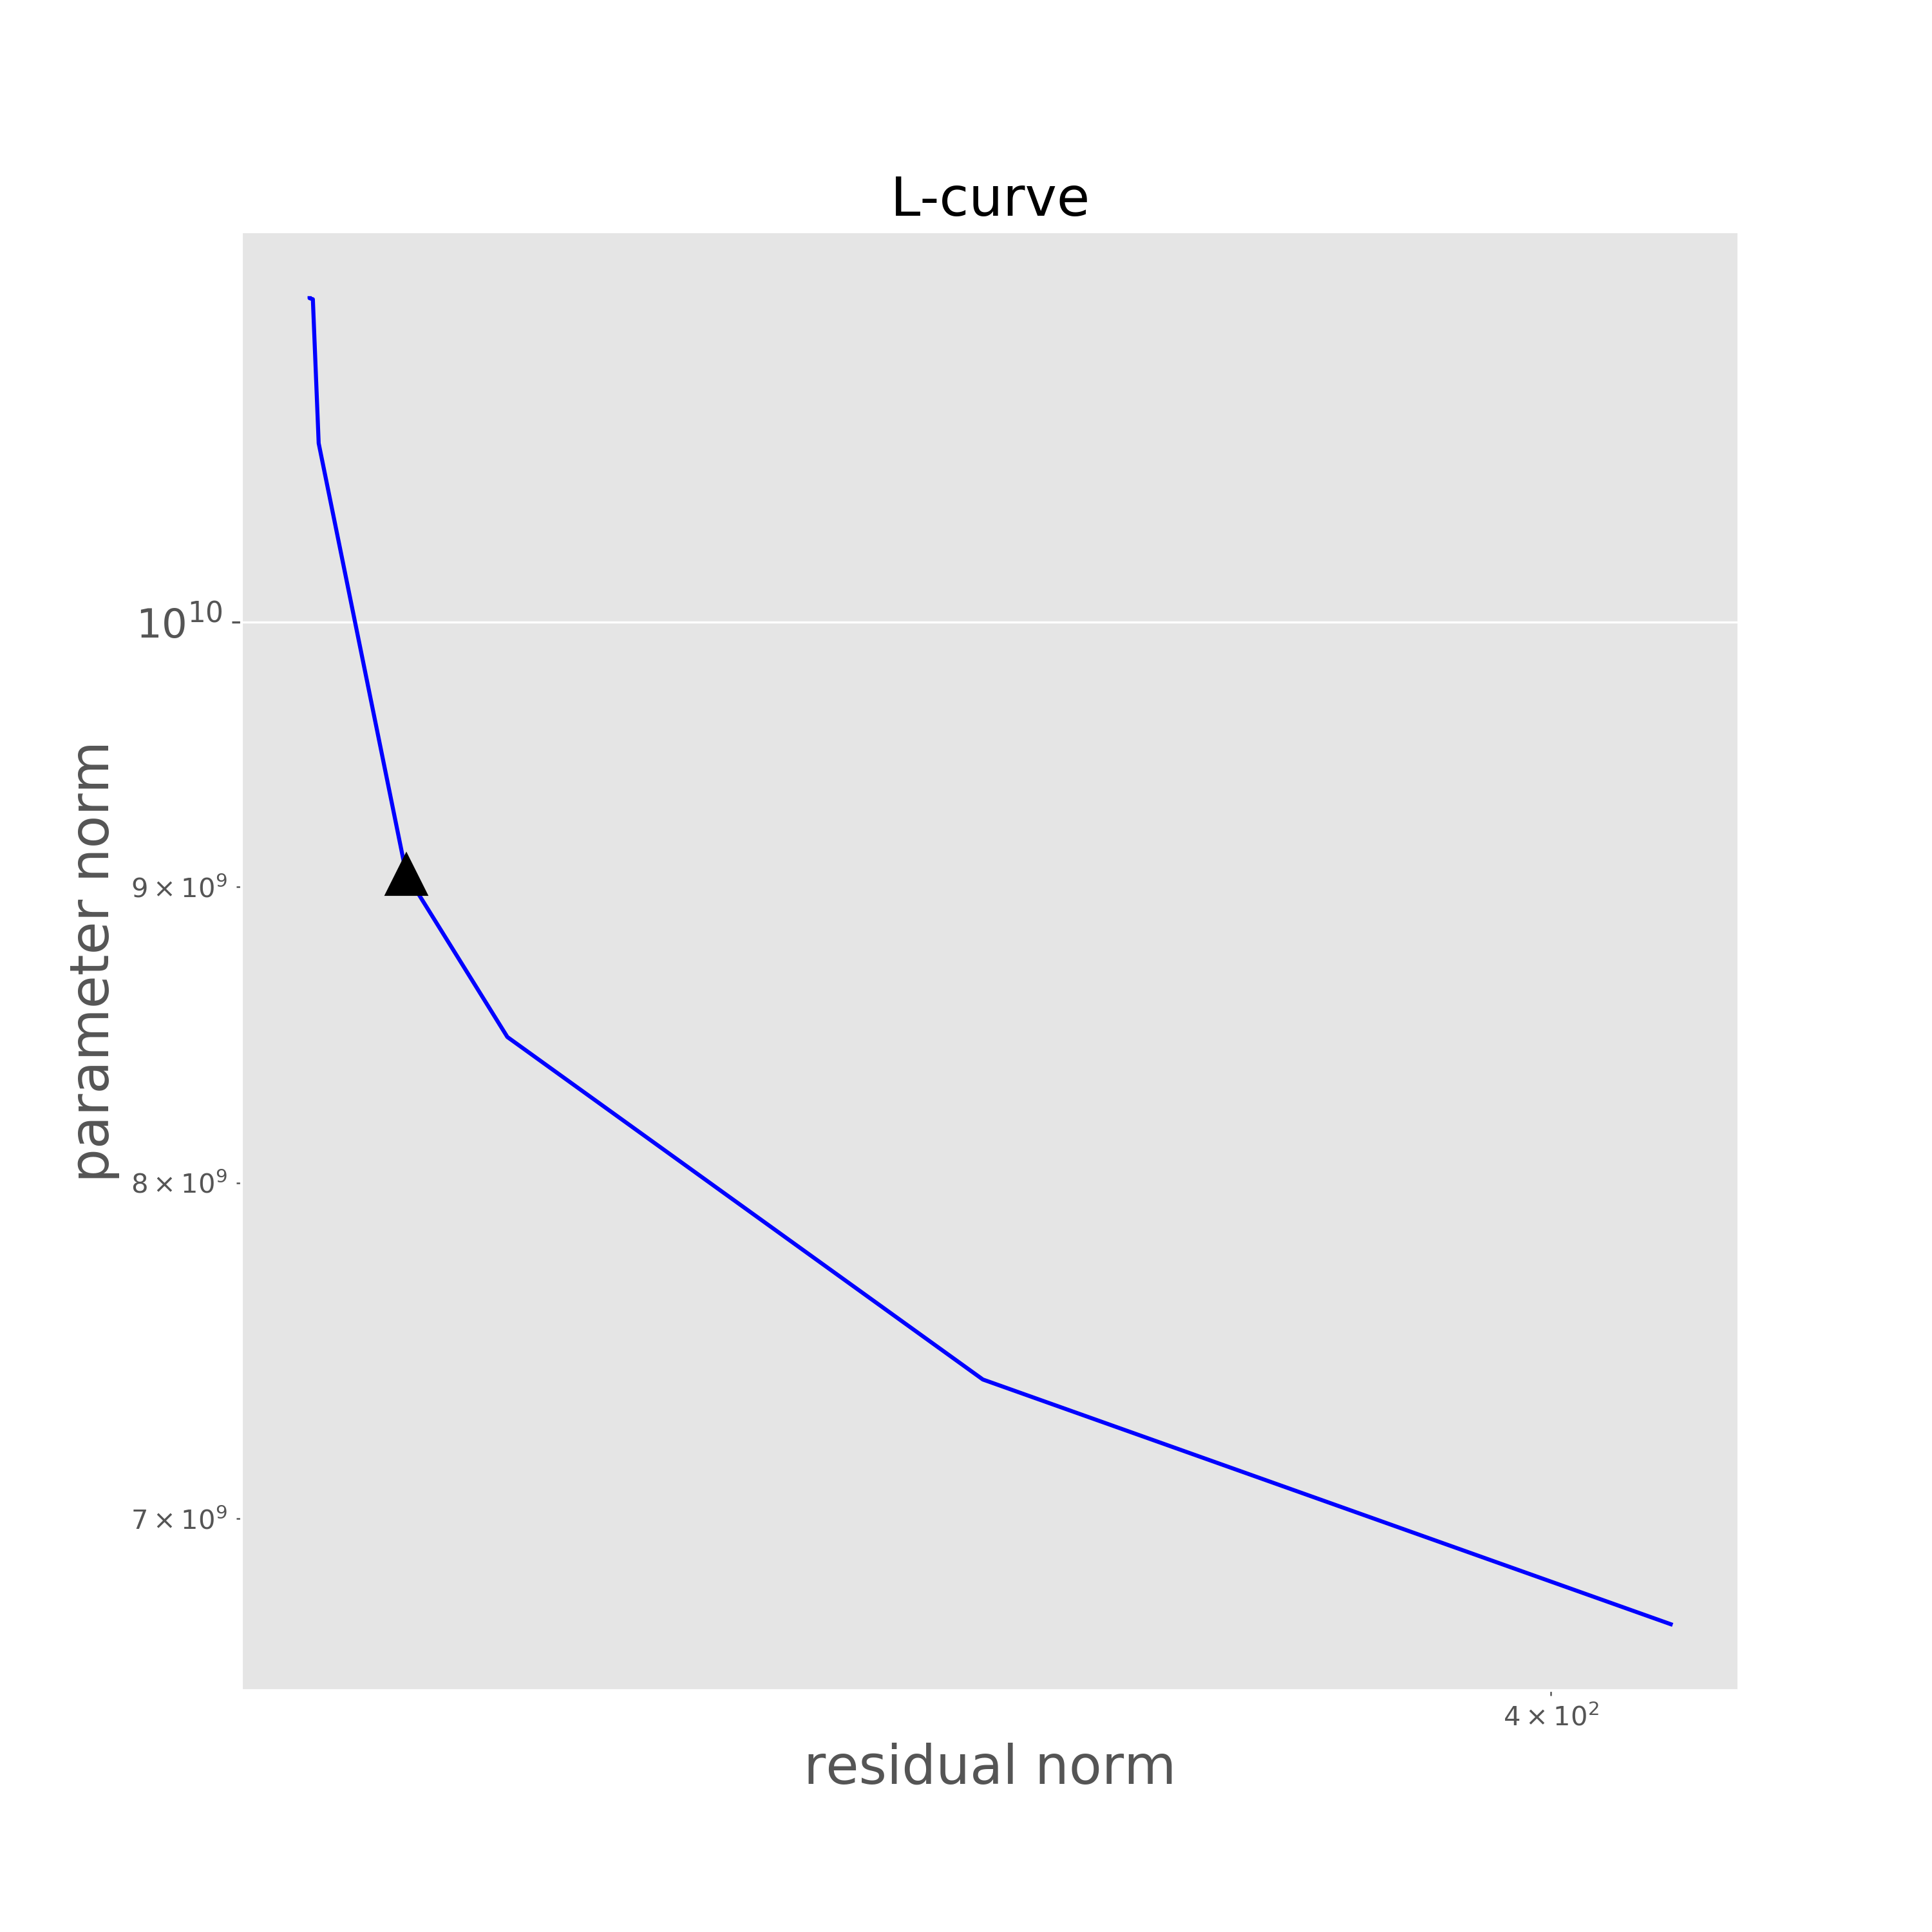
\includegraphics[width=.9\textwidth]{Fig/eqlayer/unidir_shallow_test/Lcurve_RM.png}
	\caption{Gráfico da curva-L mostrando a escolha do parâmetro de regularização $\mu$ (equação \ref{eq:positivity_goal_function}a) para o segundo teste. O triângulo em preto indica o ponto no qual foi escolhido o parâmetro igual a $350000$.}
	\label{fig:lcurve_2}
\end{figure}


\section{Fonte rasa com direção de magnetização diferente}

Neste teste simulamos a presença de uma fonte rasa com direção de magnetização diferente das demais. O prisma raso tem dimensão igual ao do teste anterior. No entanto, a direção de magnetização deste prisma é $20^\circ$ de inclinação e $-30^\circ$ de declinação, enquanto as outras fontes possuem inclinação $-25^\circ$ e declinação $30^\circ$. Os dados calculados são mostrados na figura \ref{fig:data_fitting_3}a. 

A figura \ref{fig:data_fitting_3}b mostra a anomalia de campo total predita pela camada equivalente. O mapa dos resíduos é mostrado na figura \ref{fig:data_fitting_3}c, e é definido como a diferença entre os dados observados (Figura \ref{fig:data_fitting_3}a) e os dados preditos (Figura \ref{fig:data_fitting_3}b). Os resíduos tem média igual a $-0,73$ nT e desvio padrão igual a  $12,67$ nT como mostra a figura \ref{fig:data_fitting_3}d. A direção de magnetização estimada $\bar{\mathbf{q}}$ tem inclinação $-30,4^\circ$ e declinação $27,6^\circ$. A figura \ref{fig:dist_momentos_pos_3} mostra a distribuição de momentos magnéticos positiva. A convergência do algoritmo é mostrada na figura \ref{fig:convergence_3}. A escolha do parâmetro de regularização $\mu = 3500000$ é mostrada na figura \ref{fig:lcurve_3}. Apesar da diferença em relação a direção de magnetização verdadeira, a distribuição de momentos positiva produziu um ajuste aceitável dos dados observados. Com exceção da pequena área acima da fonte rasa, a maior parte dos resíduos são próximos de $0$ nT. 

%%% Figuras teste 3
\begin{figure}
	\centering
	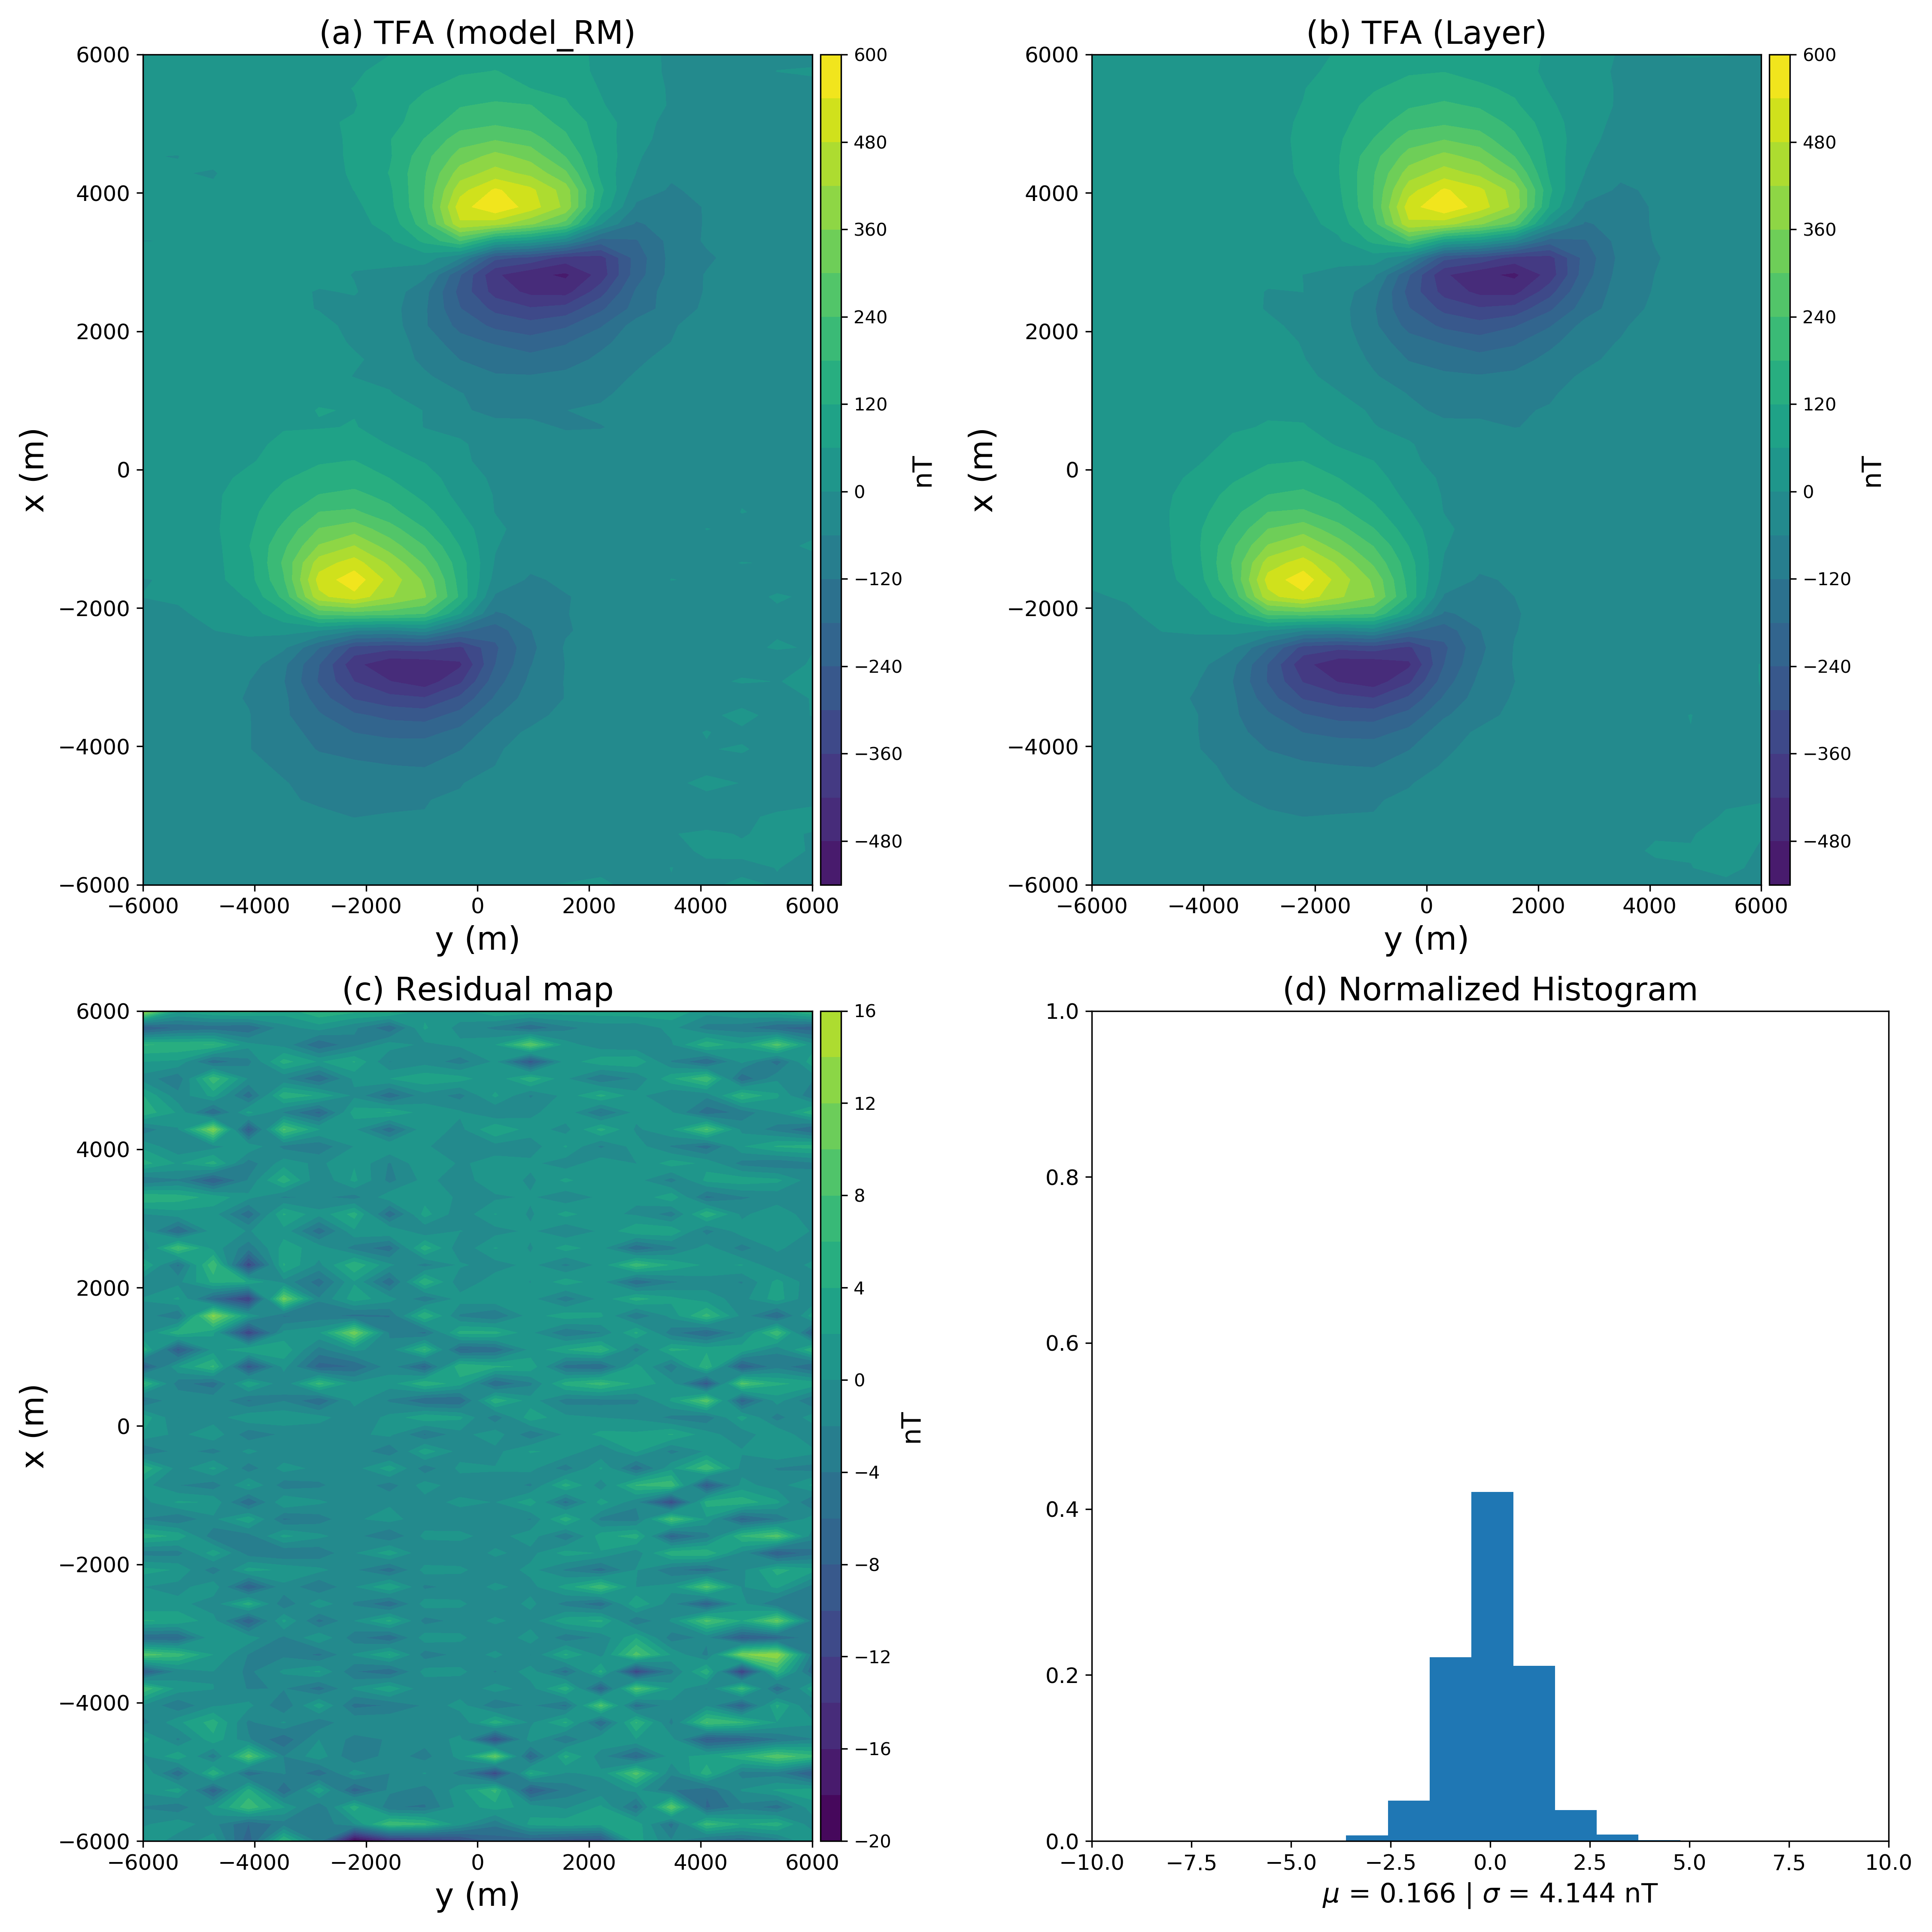
\includegraphics[width=1.1\textwidth]{Fig/eqlayer/unidir_shallow_diff_test/data_fitting_LM_NNLS_magRM.png}
	\caption{Aplicação a dados sintéticos para fonte rasa com direção de magnetização diferente. (a) Anomalia de campo total observada. (b) Dados preditos produzido pela camada equivalente. (c) Diferença entre os dados mostrados nos gráficos a e b. (d) Histograma dos resíduos.}
	\label{fig:data_fitting_3}
\end{figure}

\begin{figure}
	\centering
	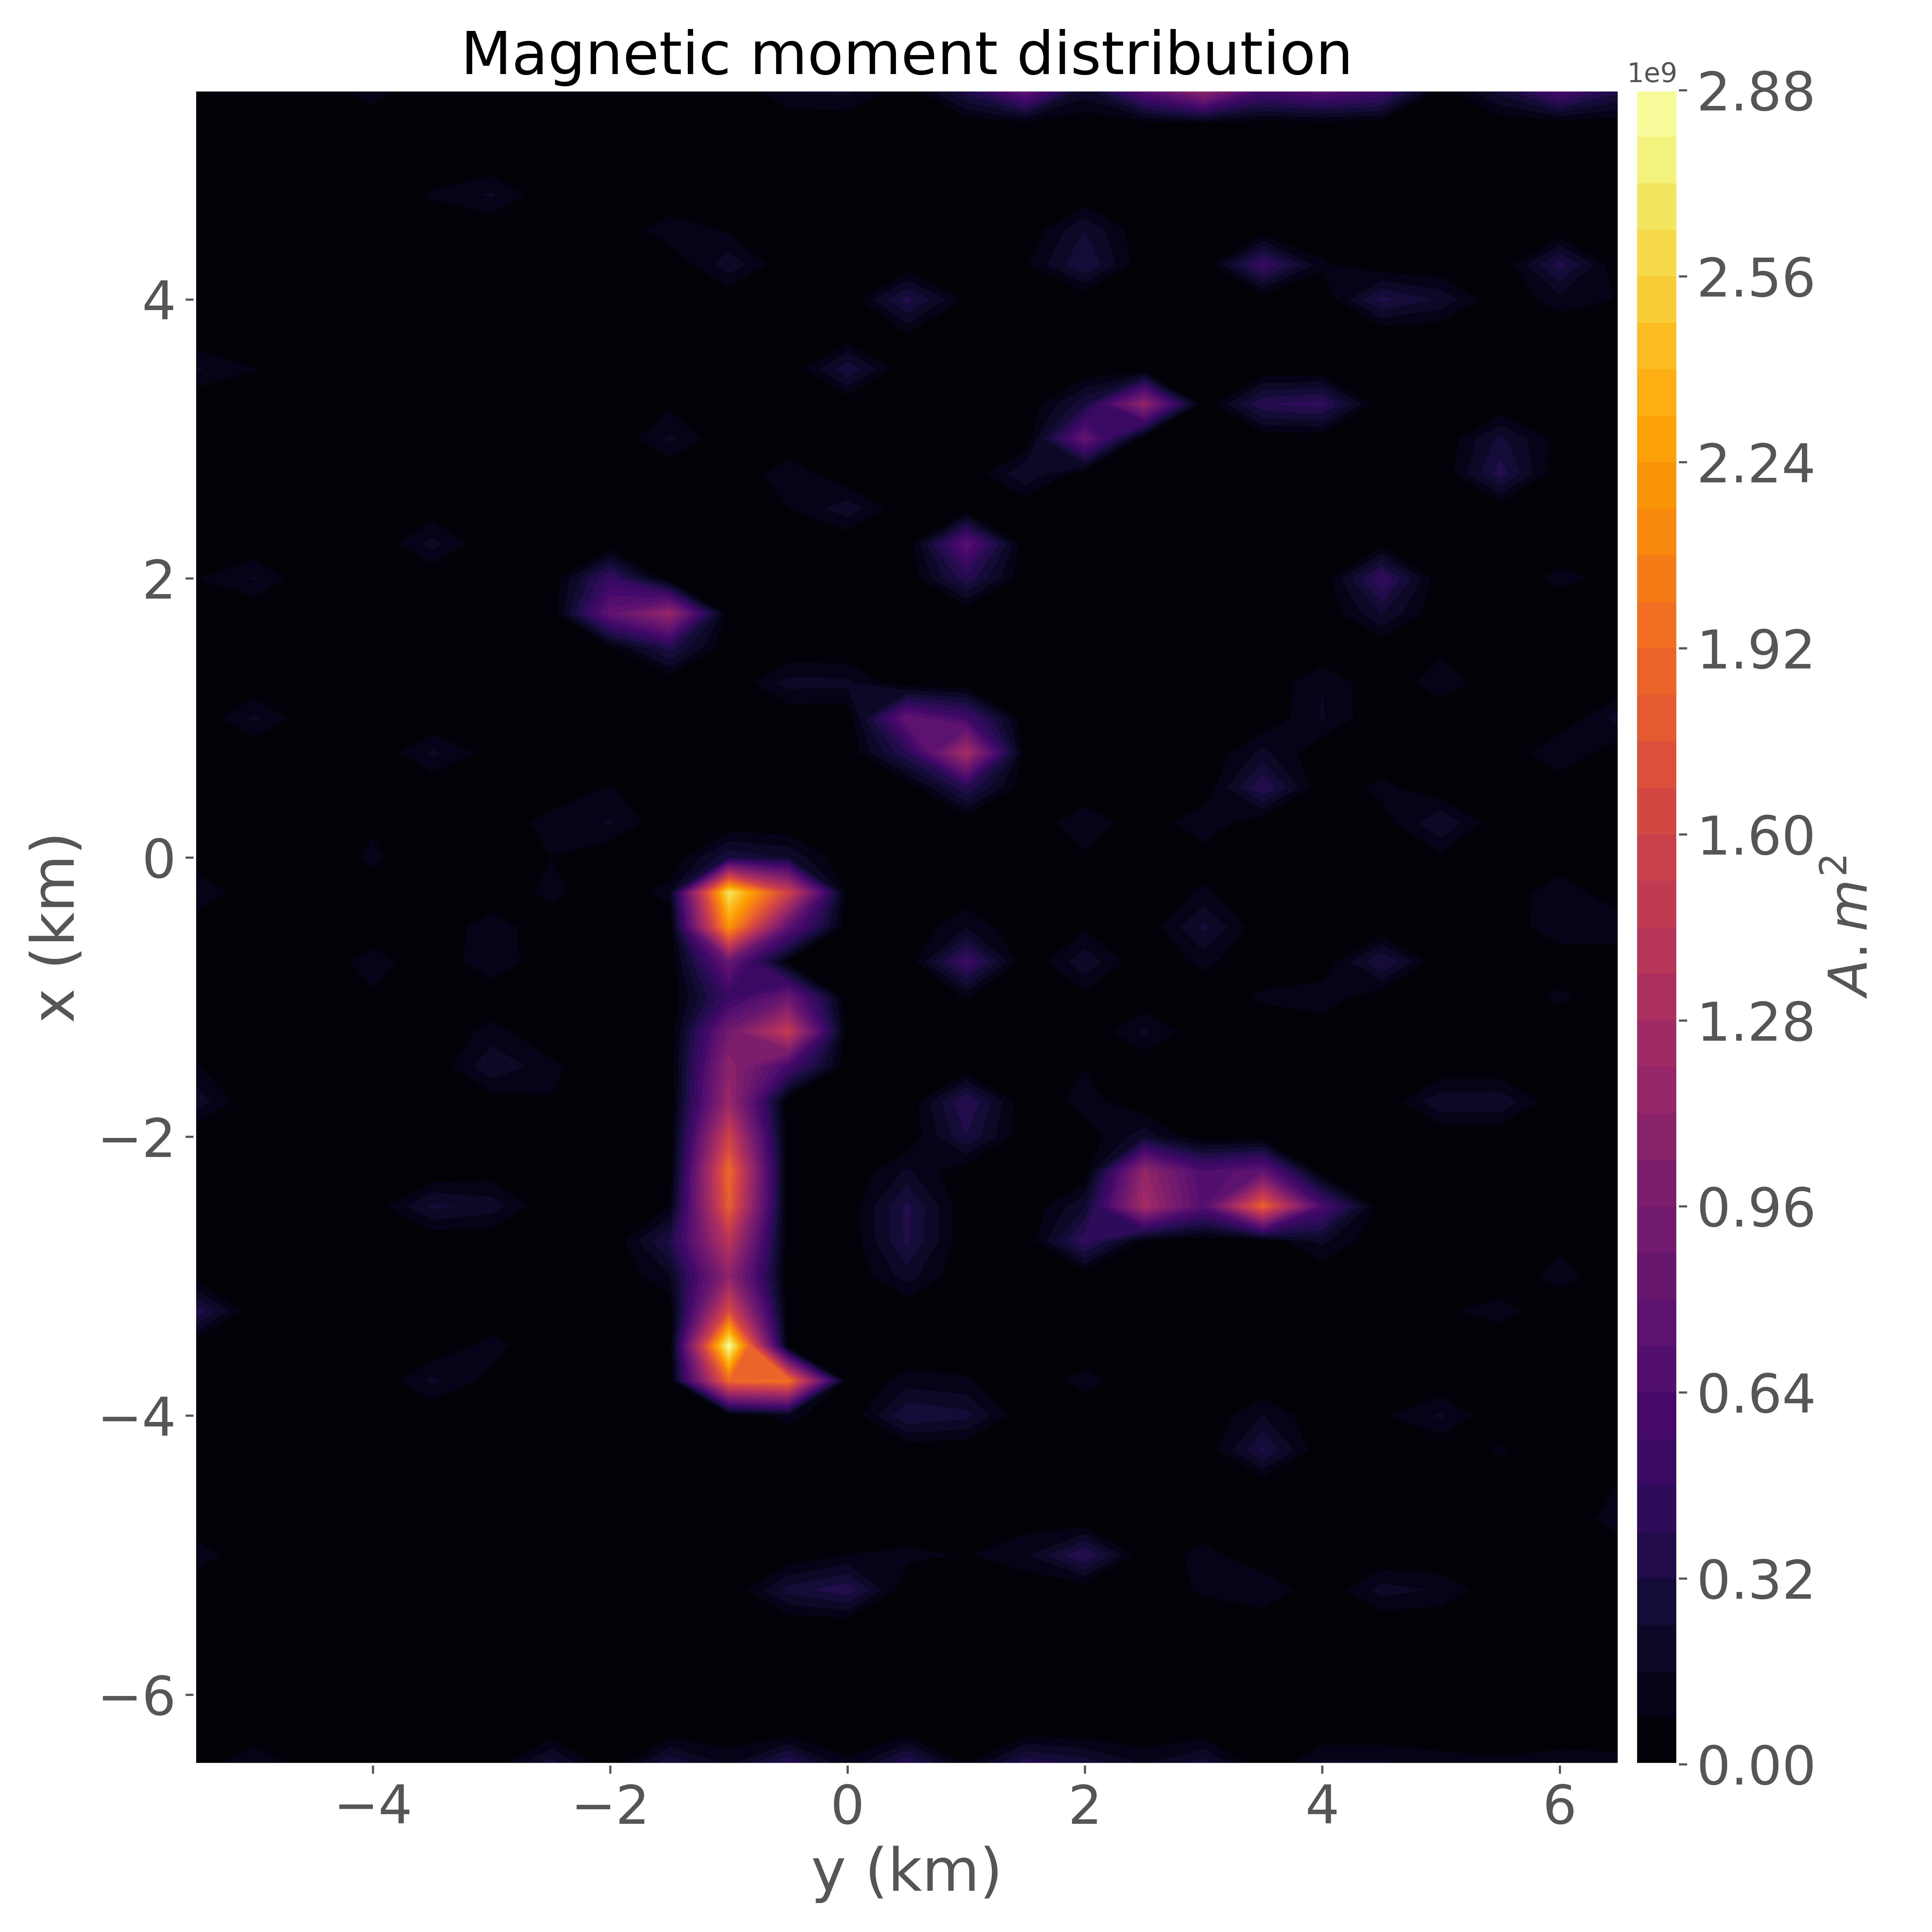
\includegraphics[width=.9\textwidth]{Fig/eqlayer/unidir_shallow_diff_test/magnetic_moment_positive_LM_NNLS_magRM.png}
	\caption{Distribuição de momentos magnéticos positiva para a aplicação a dados sintéticos para múltiplos corpos e fonte rasa com direção de magnetização diferente.}
	\label{fig:dist_momentos_pos_3}
\end{figure}

\begin{figure}
	\centering
	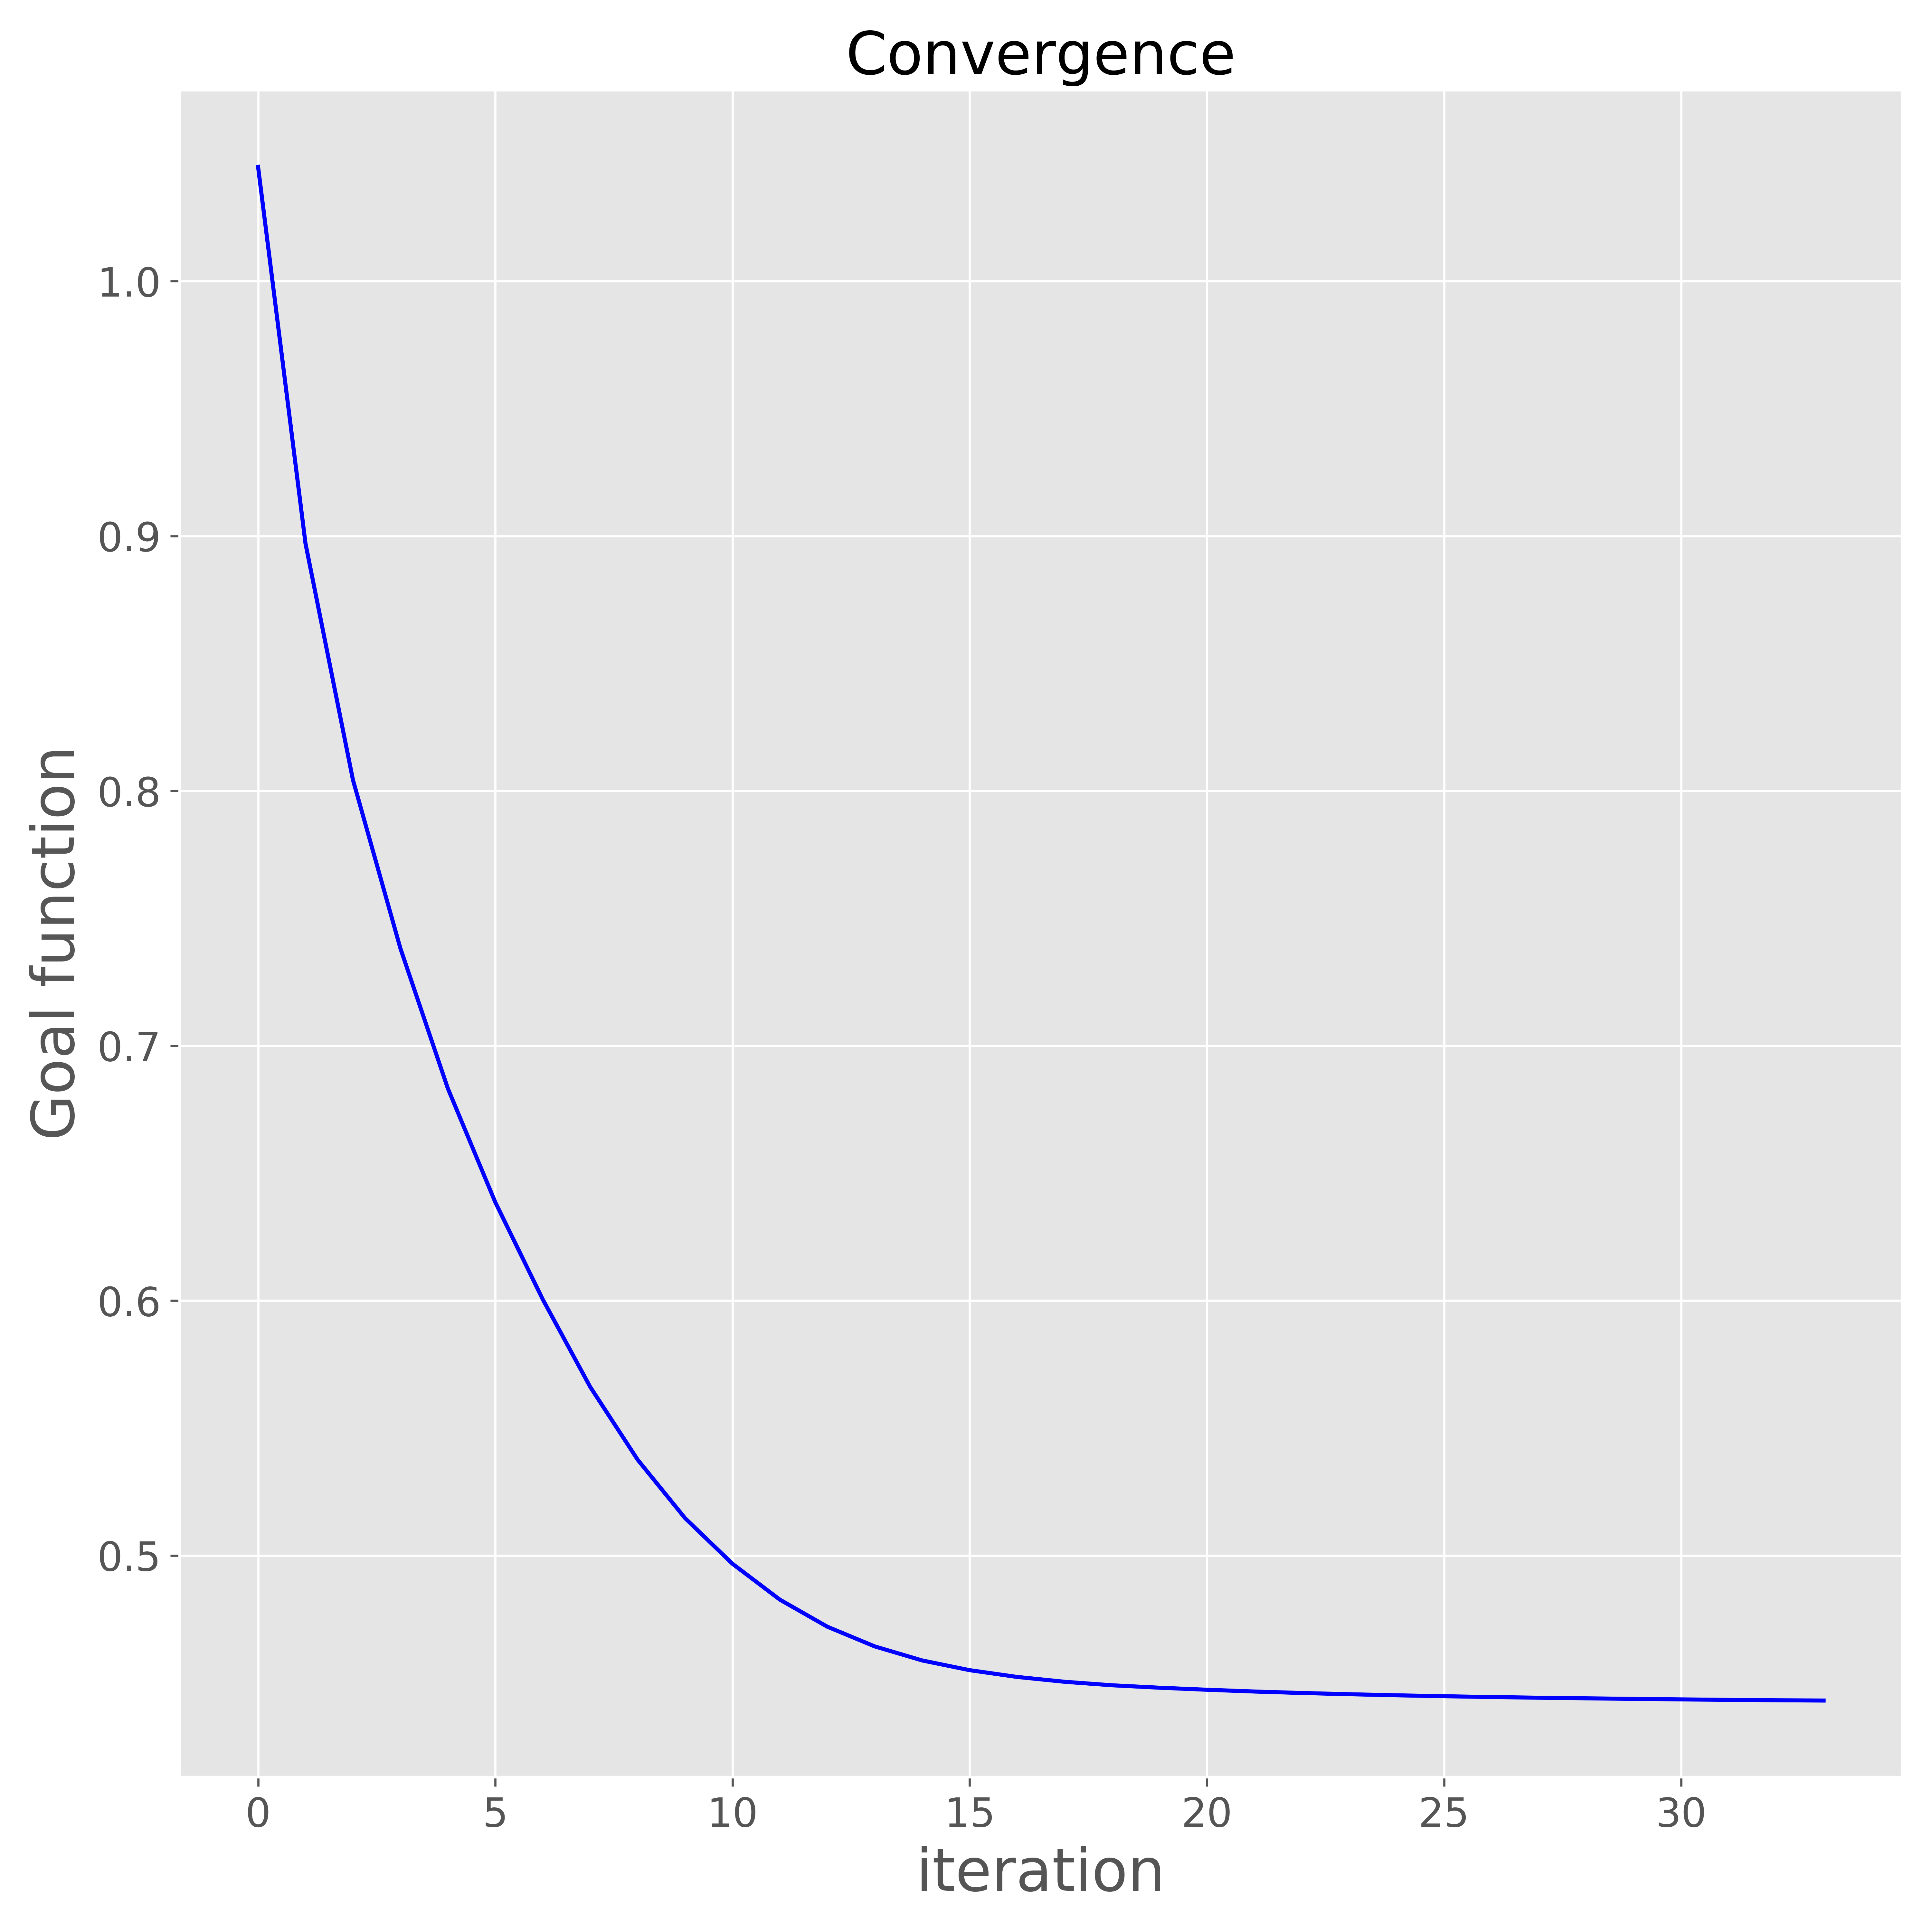
\includegraphics[width=.9\textwidth]{Fig/eqlayer/unidir_shallow_diff_test/convergence_LM_NNLS_magRM.png}
	\caption{Valor da função objetivo ao longo das iterações (equação \ref{eq:positivity_goal_function}a) mostrando a convergência do algoritmo.}
	\label{fig:convergence_3}
\end{figure}

\begin{figure}
	\centering
	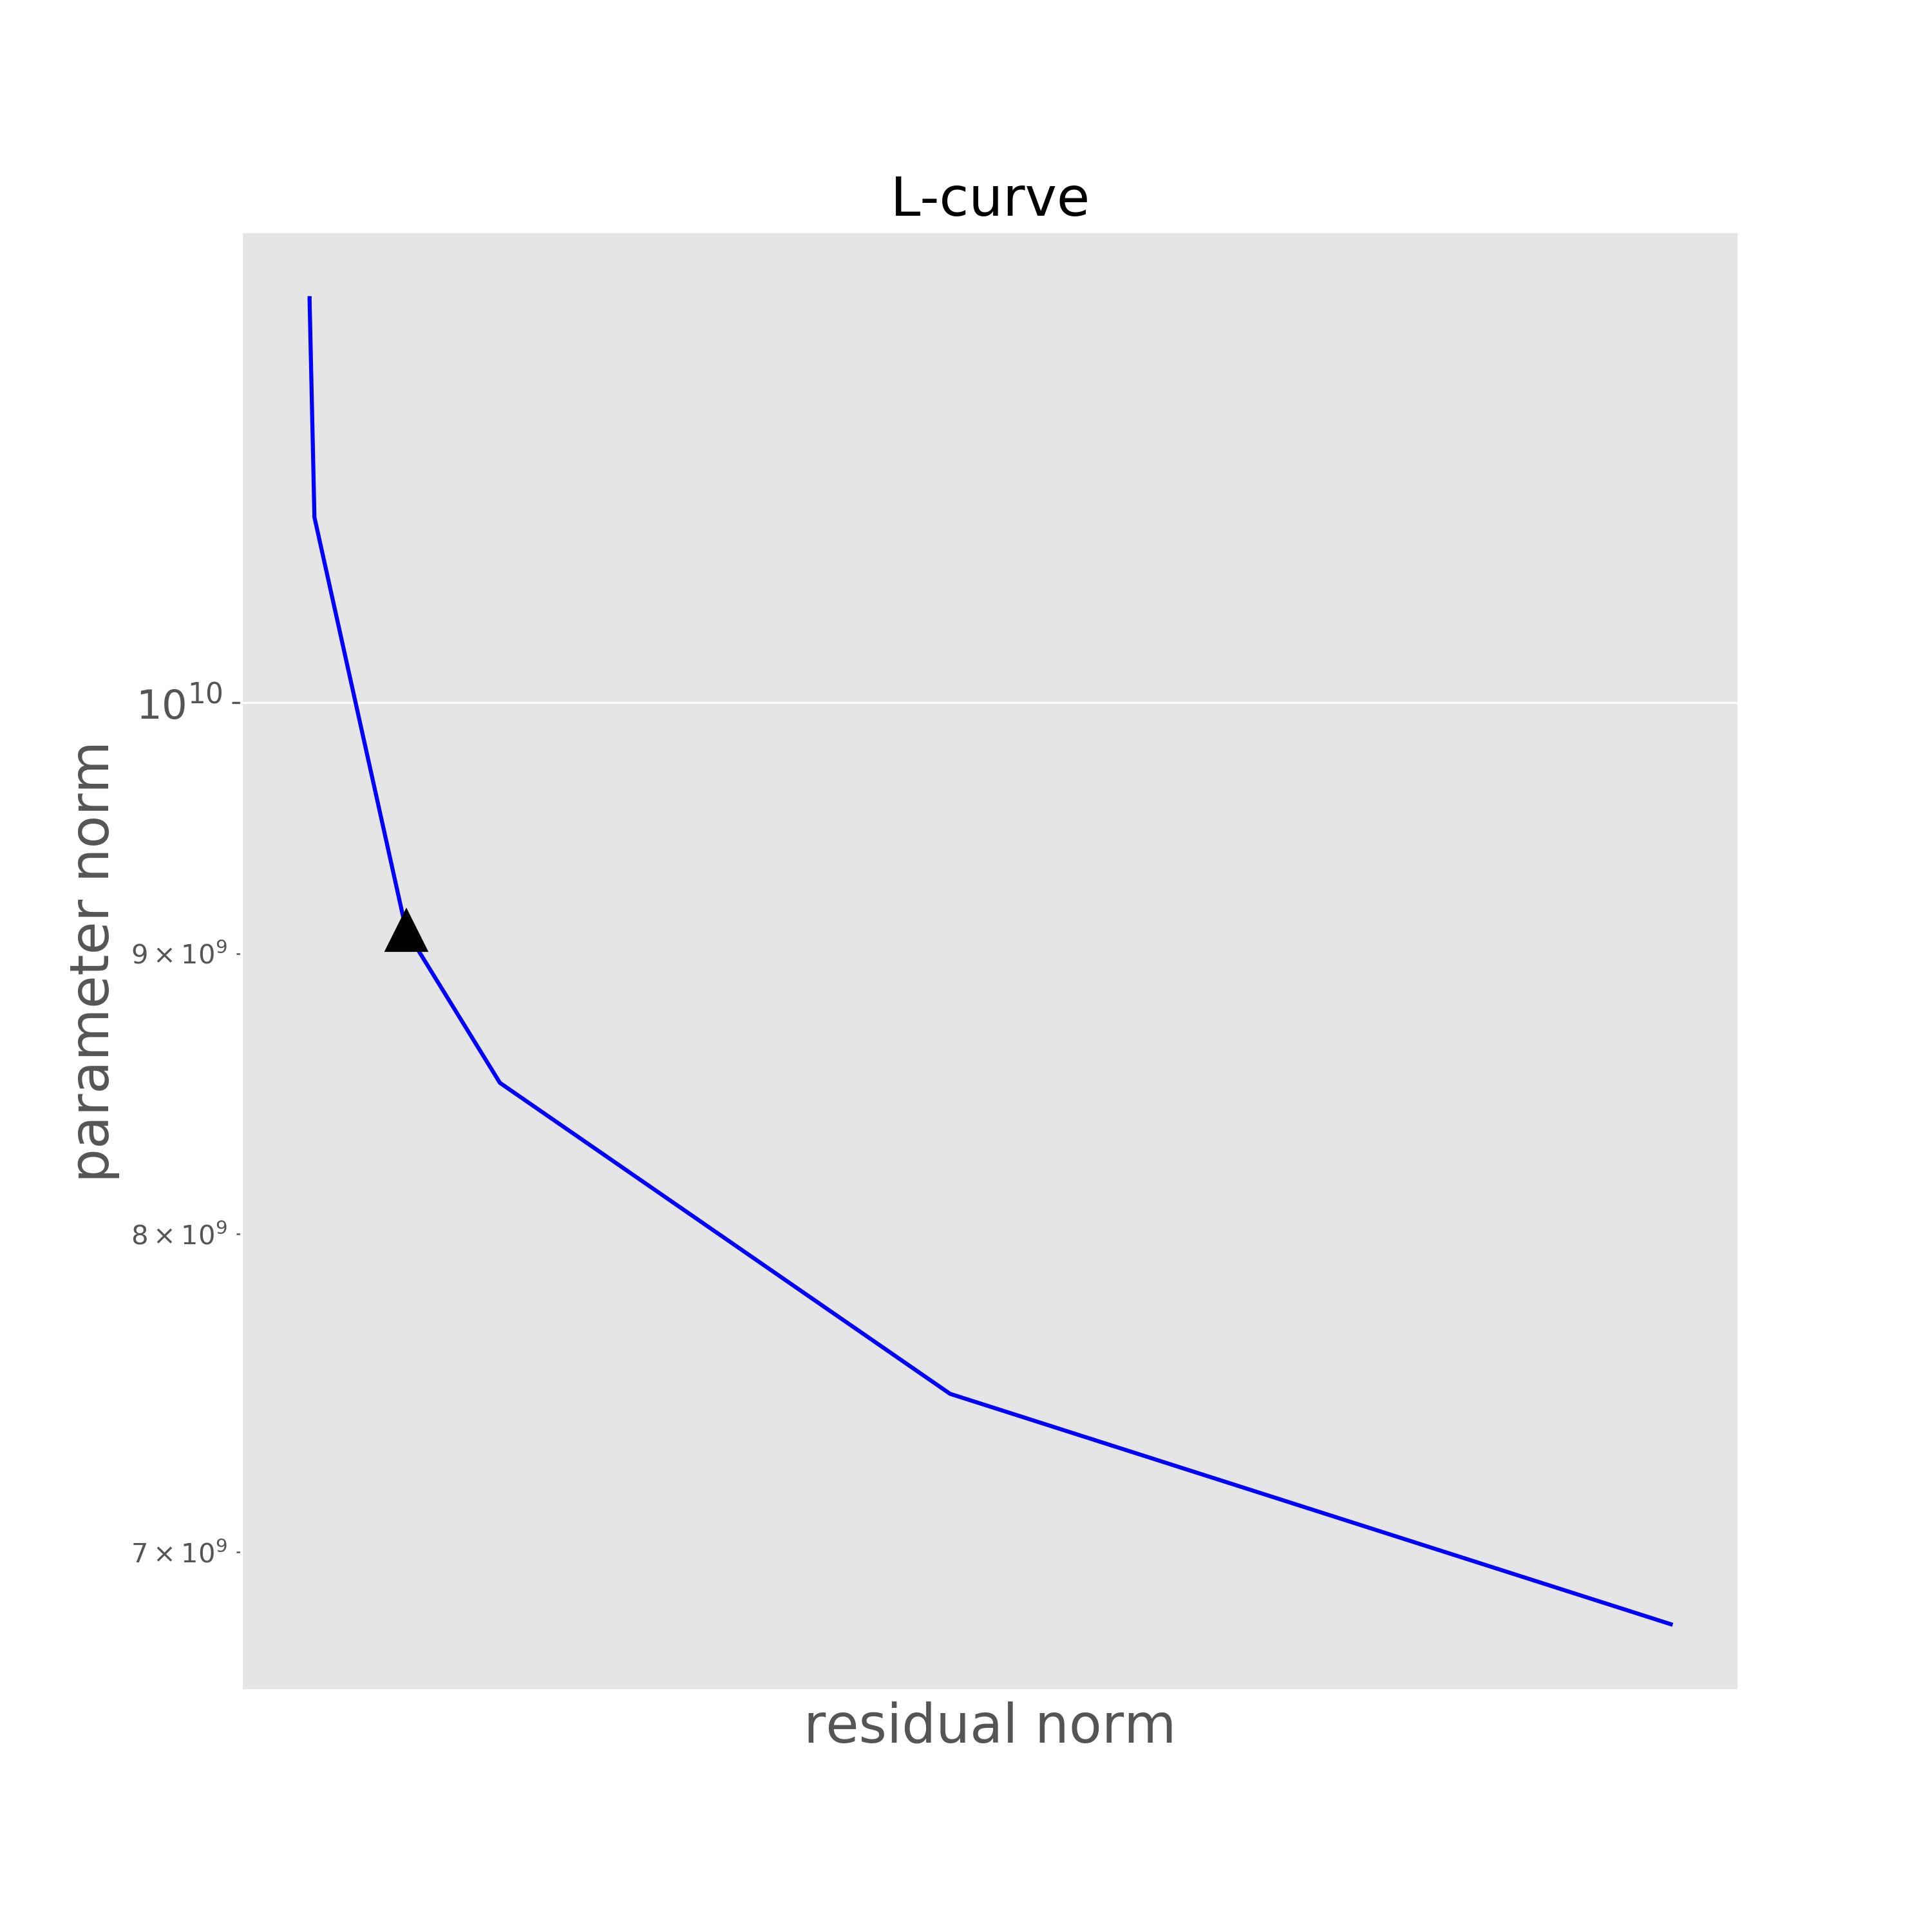
\includegraphics[width=.9\textwidth]{Fig/eqlayer/unidir_shallow_diff_test/Lcurve_RM.png}
	\caption{Gráfico da curva-L mostrando a escolha do parâmetro de regularização $\mu$ (equação \ref{eq:positivity_goal_function}a) para o terceiro teste. O triângulo em preto indica o ponto no qual foi escolhido o parâmetro igual a $350000$.}
	\label{fig:lcurve_3}
\end{figure}

%% Dados reais: Montes Claros de Goiás 
\chapter{Aplicação a dados reais: Complexo de Montes Claros de Goiás}
\label{sec:real_application}

A província alcalina de Goiás (PAGO) é uma região na parte central do Brasil onde há ocorrências de magmatismos máficos-ultramáficos alcalinos. Esta região apresenta rochas com extensas variedades petrográficas. Ao longo desta área existem complexo máficos-ultramáficos (intrusões plutônicas), intrusões alcalinas sub-vulcânicas (diátremas) e produtos vulcânicos (lava kamafugítica) com diversos diques. Alguns dos principais complexos da PAGO são: Montes Claros de Goiás, Diorama, Córrego dos Bois, Morro do Macaco e Fazenda Buriti. Estas intrusões alcalinas são cercadas por um embasamento Pré-cambriano e rochas sedimentares do Fanerozóico da bacia do Paraná \citep{junqueira_brod_2005,carlson_etal_2007,marangoni_mantovani_2013,dutra_etal_2014}. Estudos recentes indicam que tais intrusões possuem marcantes componentes de magnetização remanente \citep{marangoni_mantovani_2013,oliveirajr_etal_2015,marangoni_etal_2016,zhang_etal_2018}.

Esta região foi alvo de um levantamento aeromagnético com espaçamento entre as linhas norte-sul de $\sim 500$ m e de $\sim 8$ ao longo de cada linha, a uma altura constante de $100$ m acima do terreno. A direção do campo geomagnético para esta área era, respectivamente, de $-19.5^\circ$ e $-18.5^\circ$ para inclinação e declinação na época do levantamento. Invertemos os dados de anomalia de campo total para o complexo alcalino de Montes Claros de Goiás (Figura \ref{fig:data_fitting_real}a). Com o intuito de acelerar o processo de inversão, decimamos os dados ao longo da linha de voo, resultando em um grid de $55 \times 32$ pontos (um total de $N=1787$ observações). Esta nova configuração resulta em um espaçamento do grid de aproximadamente $300$ m e $500$ m ao longo dos eixos $x$ e $y$, respectivamente. Geramos uma camada equivalente composta por um grid de $55 \times 32$ dipolos (um total de $M=1787$ fontes equivalentes) posicionados a uma profundidade de $840$ m abaixo do plano de observação ($\sim 2$ vezes o maior espaçamento do grid). O algoritmo começa com uma aproximação inicial de $-70^\circ$ e $50^\circ$ para inclinação e declinação, respectivamente. A figura \ref{fig:data_fitting_real}b mostra os dados preditos produzidos pela camada equivalente. A figura \ref{fig:data_fitting_real}c mostra o mapa dos resíduos definido como a diferença entre os dados observados (Figura \ref{fig:data_fitting_real}a) e os dados preditos (Figura \ref{fig:data_fitting_real}b). Note que, dois locais na figura \ref{fig:data_fitting_real}c apresentam marcantes resíduos que, aparentemente, podem indicar a existência de fontes geológicas rasas. No entando, o histograma dos resíduos (Figura \ref{fig:data_fitting_real}d) é aceitável apresentando média de $-14.52$ nT (aproximadamente $0.1\% $ do valor máximo de anomalia de campo total) e desvio padrão de $312.28$ nT ($\sim 2 \% $ do valor máximo de anomalia de campo total). A direção de magnetização estimada $\bar{\mathbf{q}}$ tem inclinação $-50.2^\circ$ e declinação $34.9^\circ$. As figuras \ref{fig:dist_momentos_pos_real} e \ref{fig:convergence_real} mostram a distribuição de momentos magnéticos estimada $\bar{\mathbf{p}}$ e a convergência do algoritmo. Checamos a qualidade da direção de magnetização estimada calculando a redução ao polo da anomalia de campo total observada. Notamos que a anomalia reduzida ao polo (Figura \ref{fig:rtp_mc_data}) exibe valores predominantemente positivos e decai a zero quando se aproxima da borda da área de estudo. Por esta razão, consideramos que a direção de magnetização estimada leva a uma satisfatória anomalia reduzida ao polo. Concluimos com estes resultados que a distribuição de momentos magnéticos positiva e a direção de magnetização estimada produz um ajuste aceitável dos dados observados. A direção de magnetização estimada sugere também a existência de magnetização remanente para as intrusões na área de estudo.  

%% Figuras para aplicação a dados reais 
\begin{figure}
	\centering
	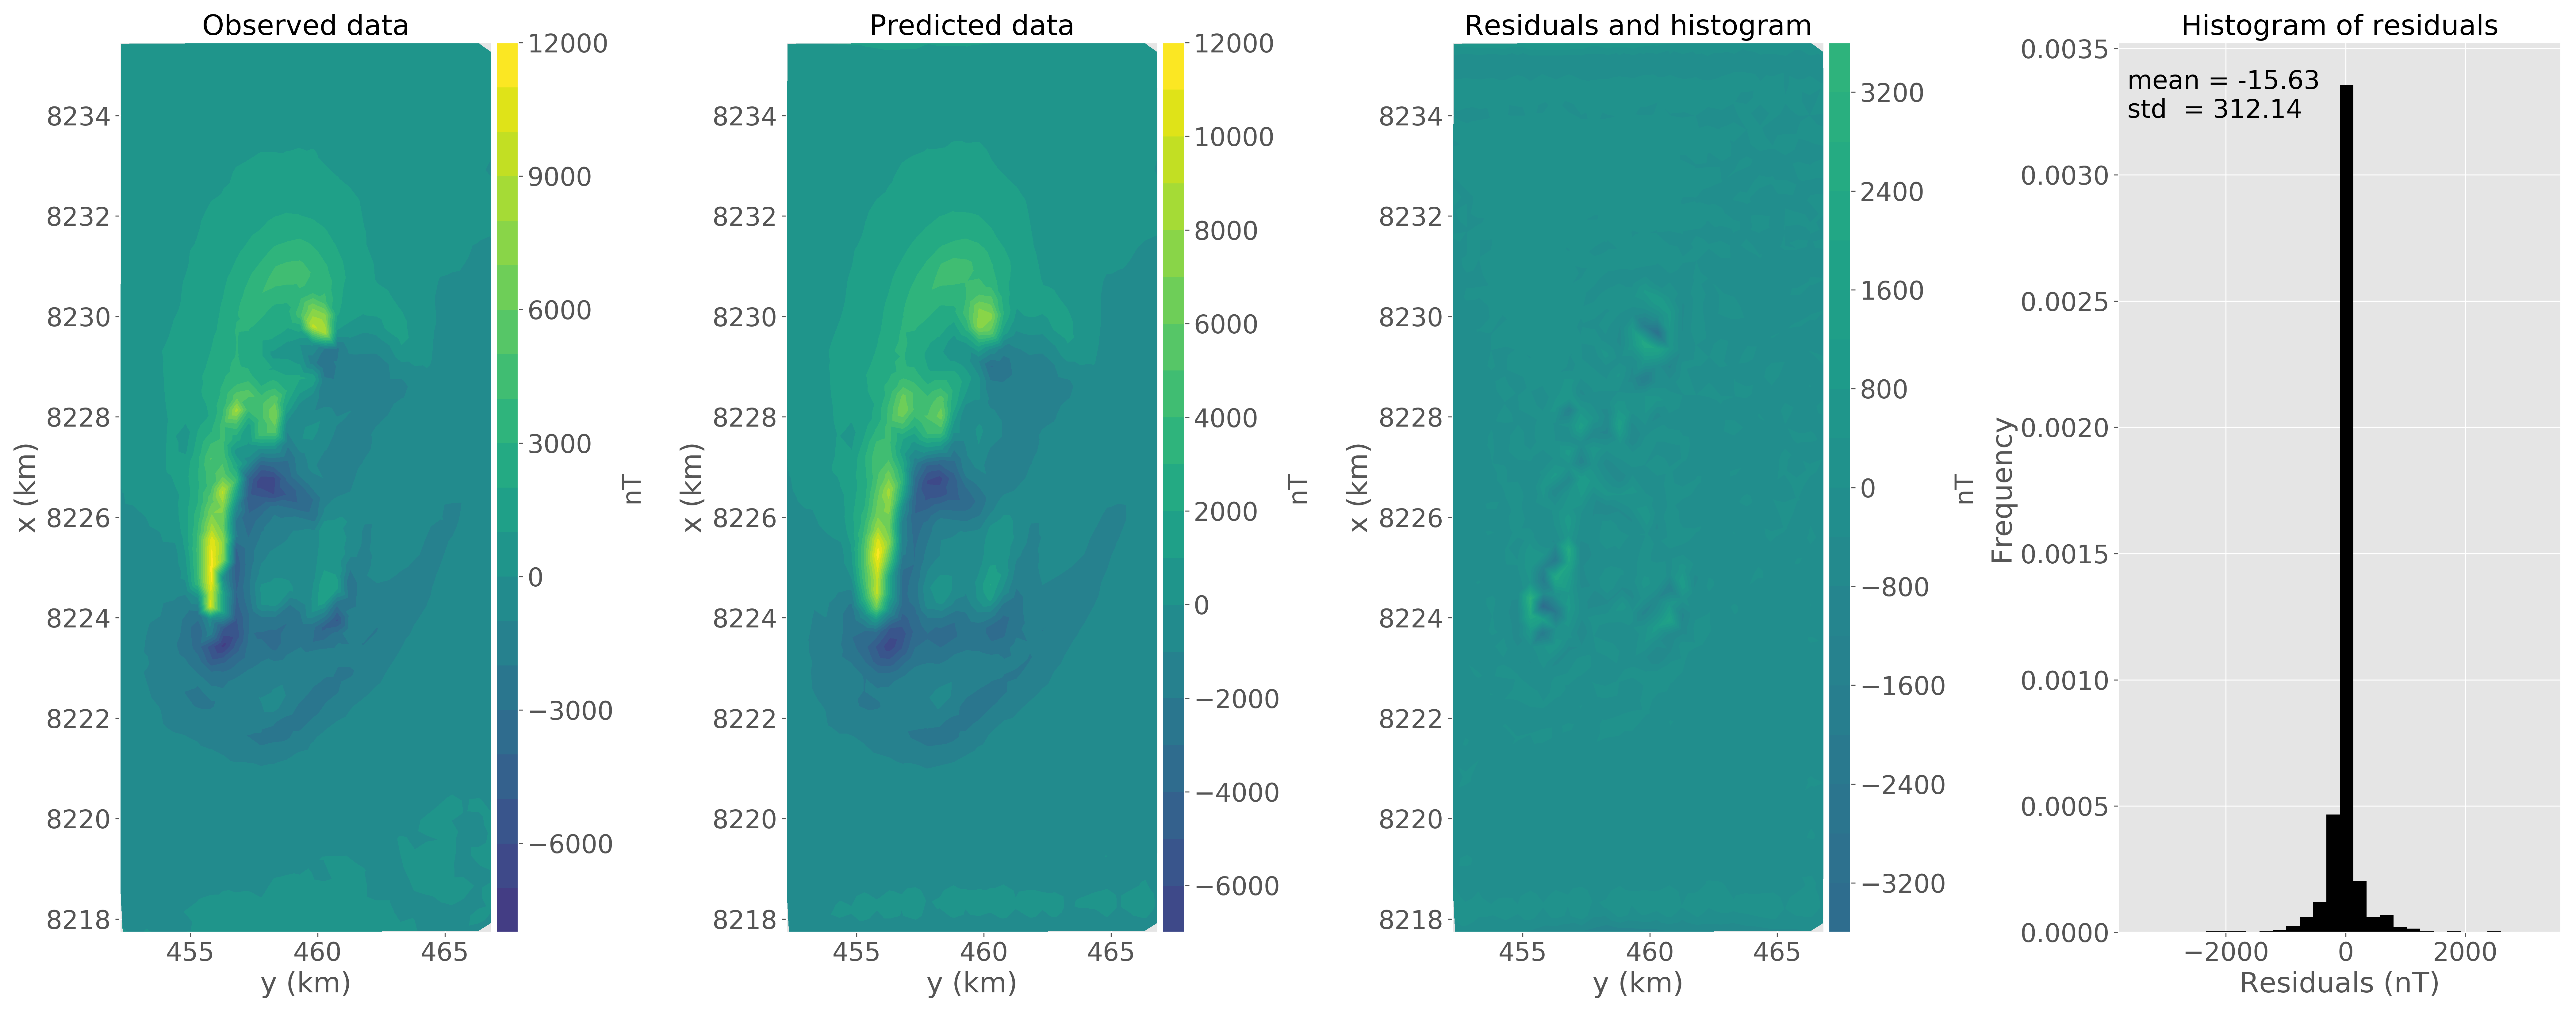
\includegraphics[width=1.1\textwidth]{Fig/eqlayer/field_data_montes_claros/data_fitting_LM_NNLS_montesclaros.png}
	\caption{Aplicação a dados reais para o complexo de Montes Claros de Goiás. (a) Anomalia de campo total observada. (b) Dados preditos produzido pela camada equivalente. (c) Diferença entre os dados mostrados nos gráficos a e b. (d) Histograma dos resíduos.}
	\label{fig:data_fitting_real}
\end{figure}

\begin{figure}
	\centering
	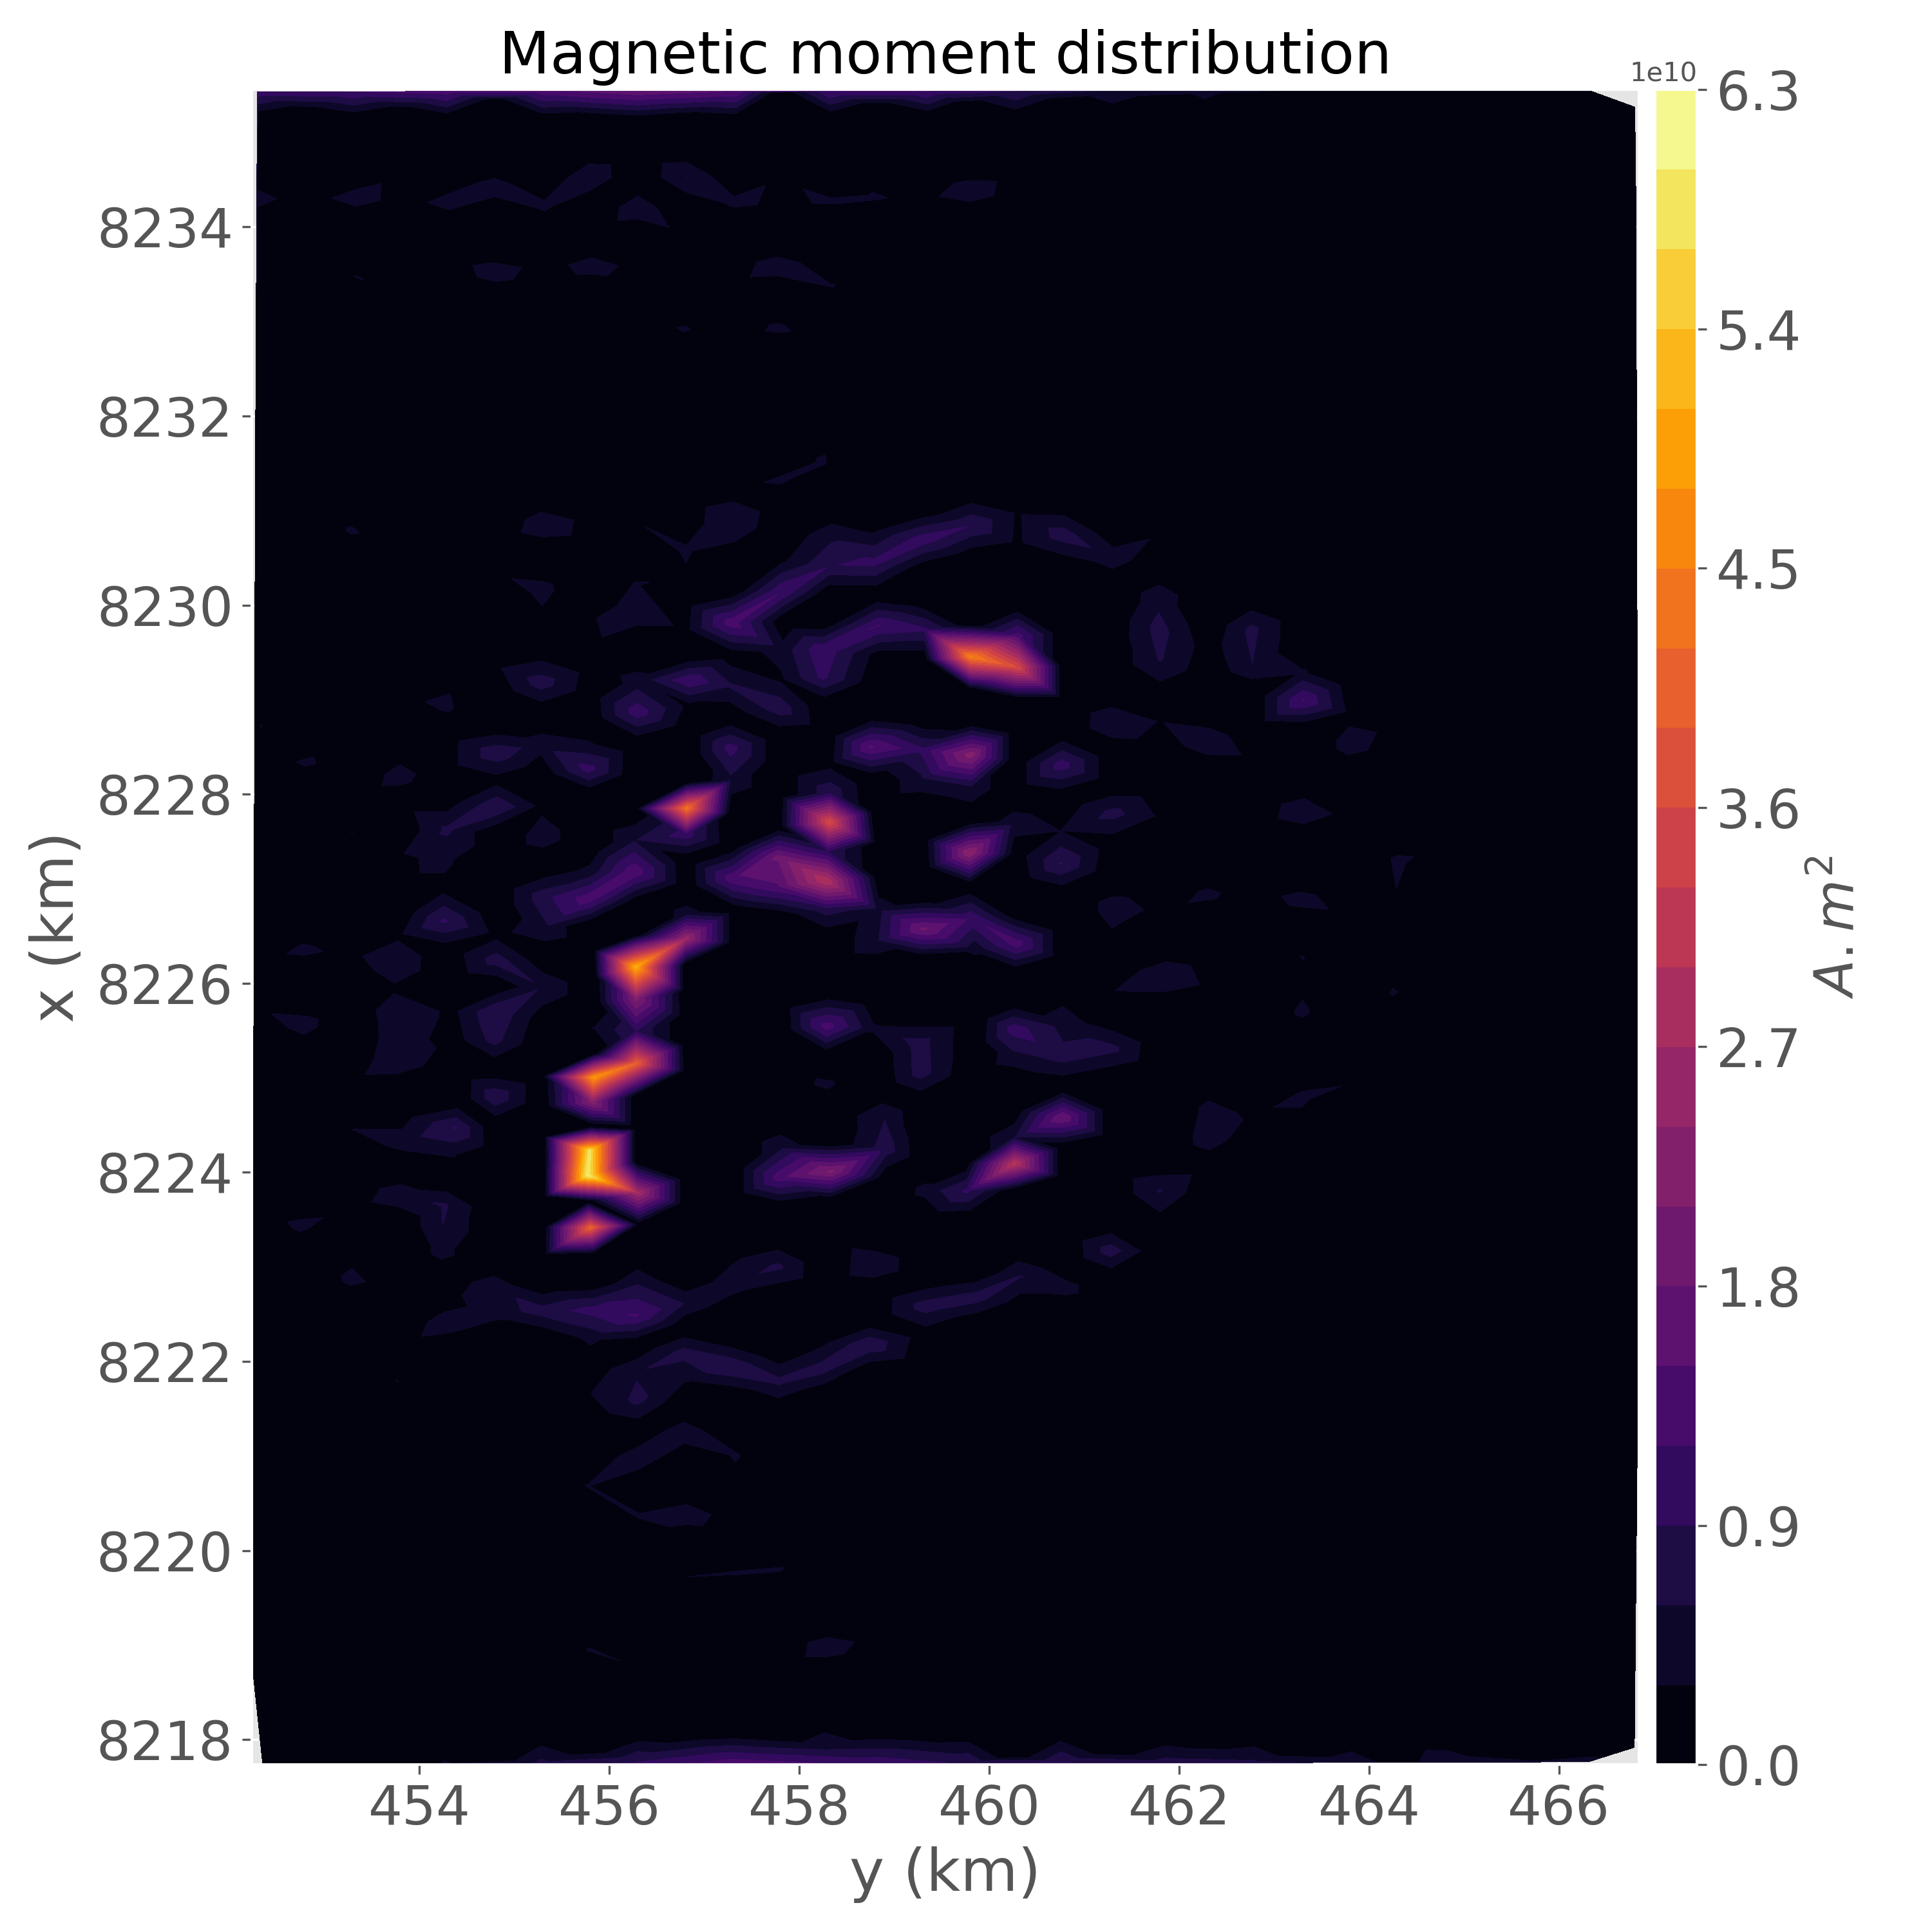
\includegraphics[width=.9\textwidth]{Fig/eqlayer/field_data_montes_claros/magnetic_moment_positive_LM_NNLS_montesclaros.png}
	\caption{Distribuição de momentos magnéticos positiva para a aplicação a dados reais no complexo de Montes Claros de Goiás.}
	\label{fig:dist_momentos_pos_real}
\end{figure}

\begin{figure}
	\centering
	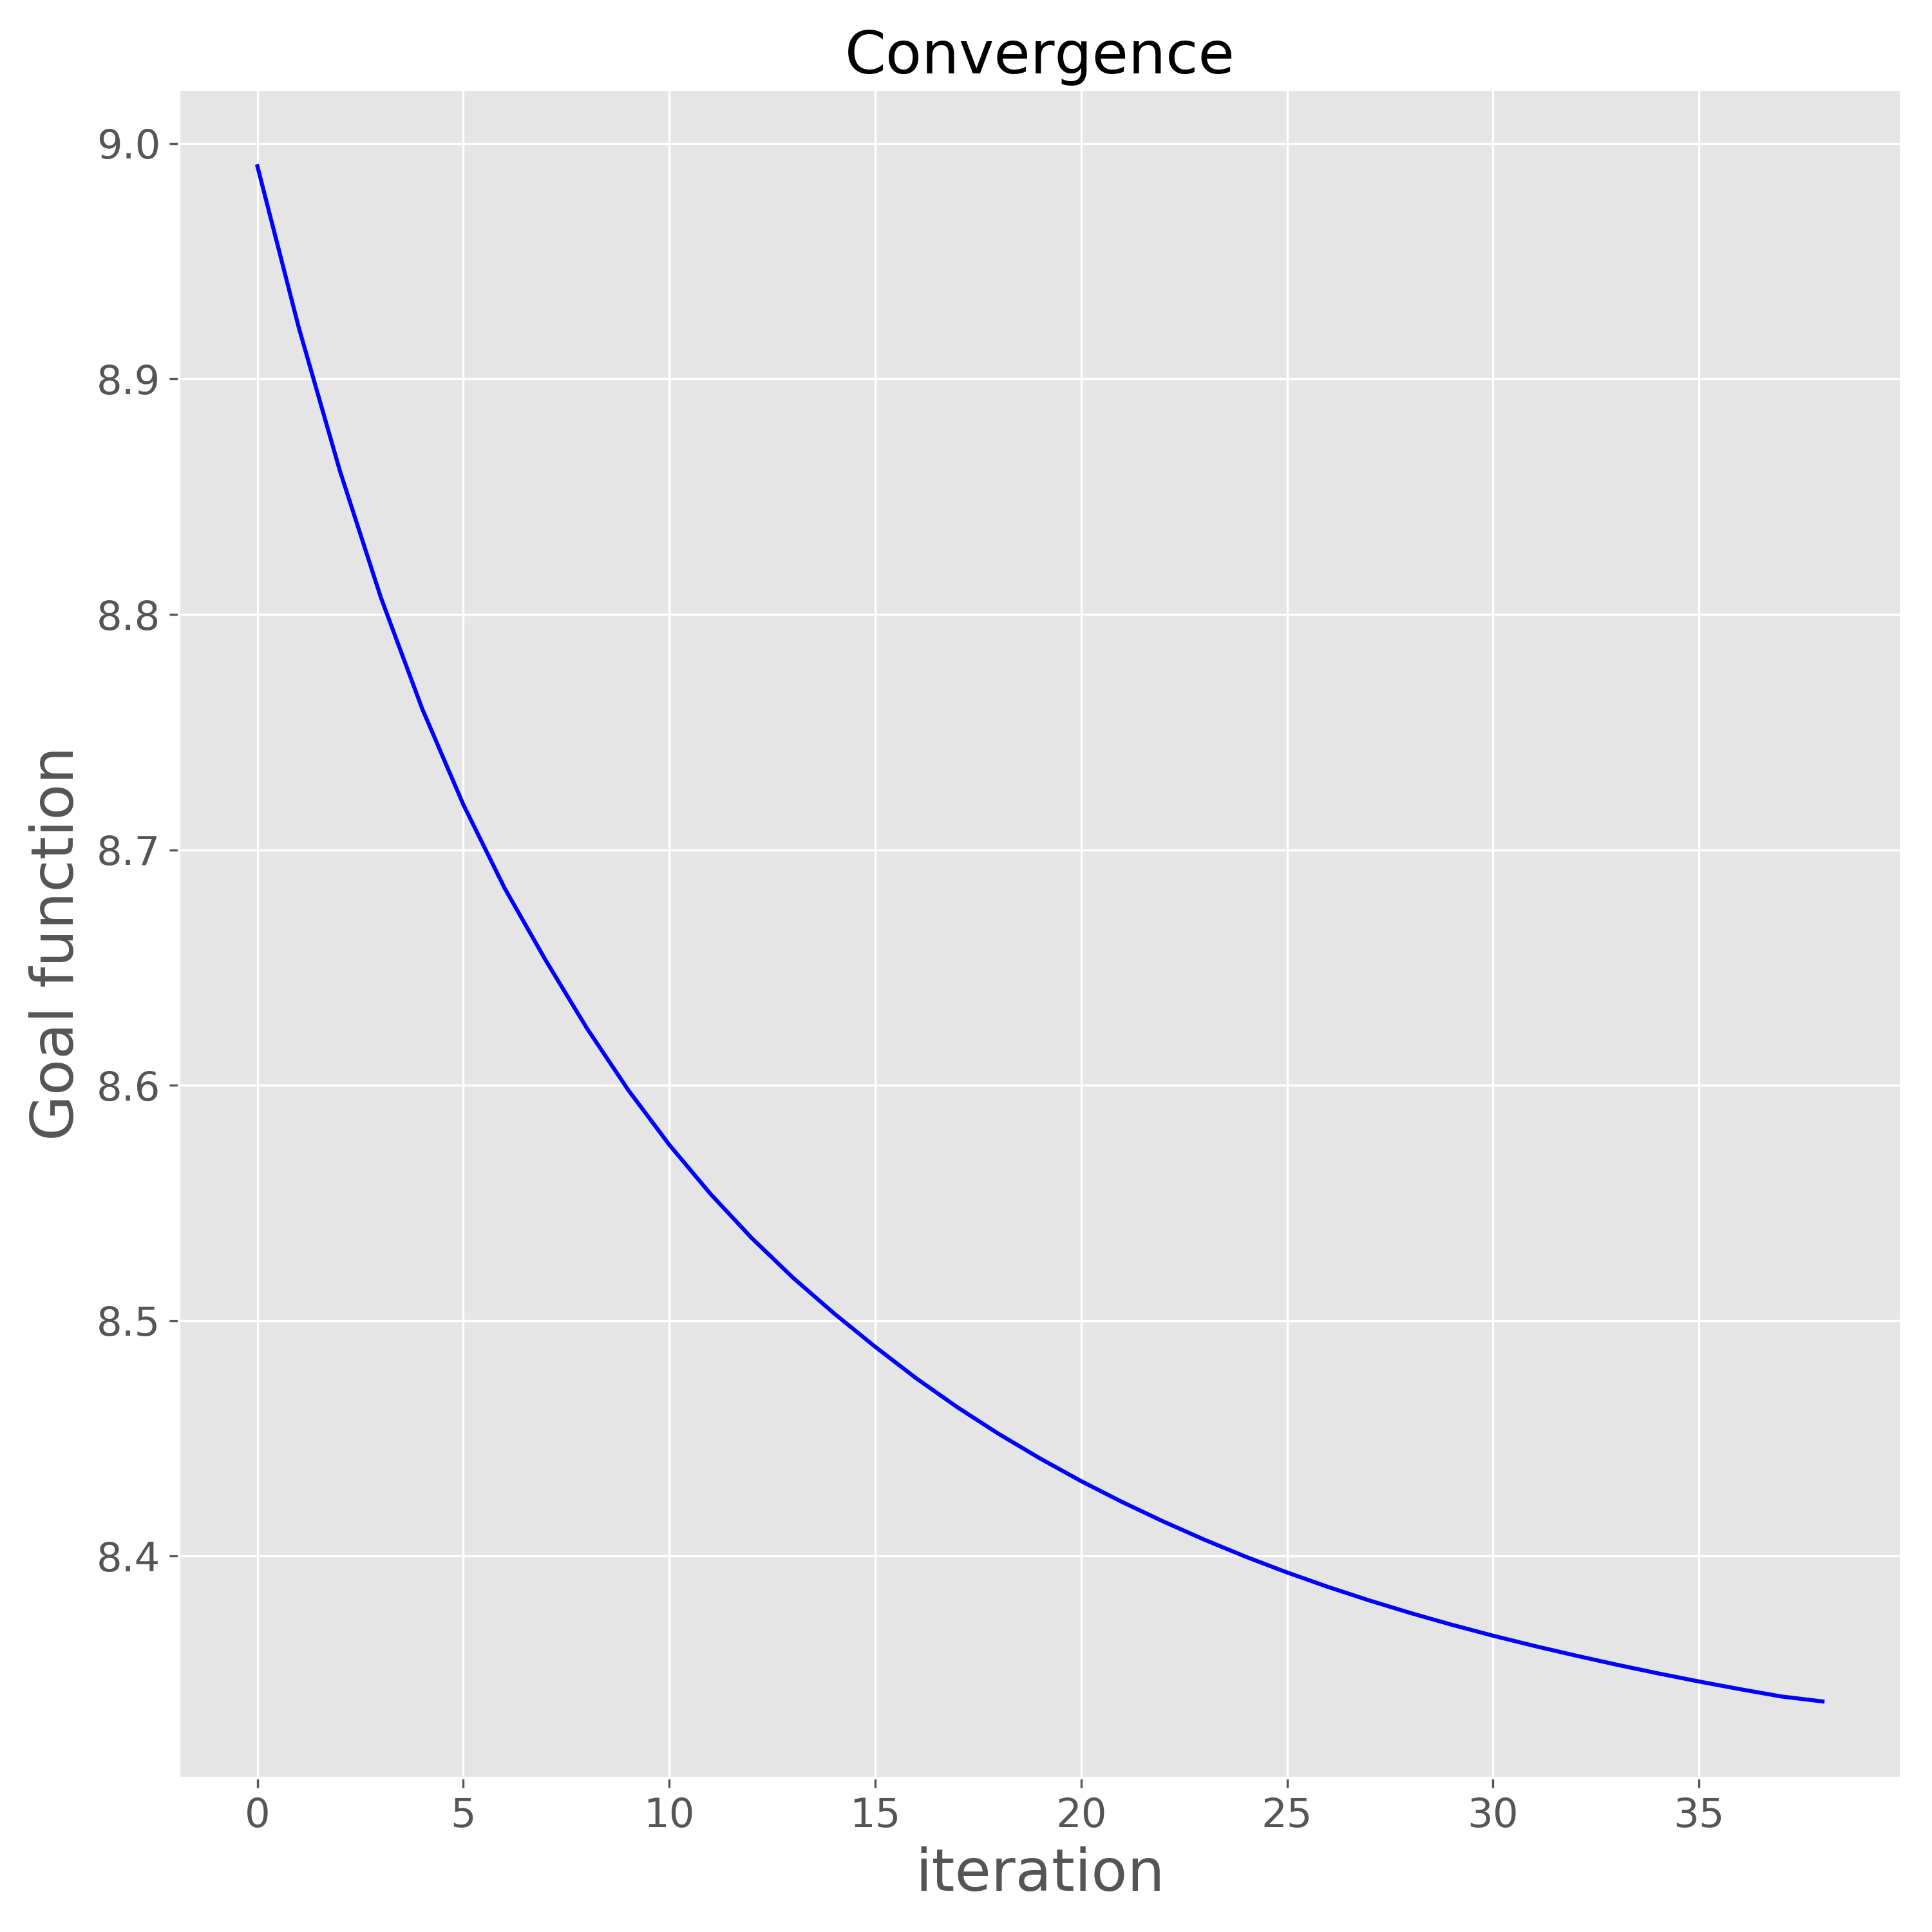
\includegraphics[width=.9\textwidth]{Fig/eqlayer/field_data_montes_claros/convergence_LM_NNLS_montesclaros.png}
	\caption{Valor da função objetivo ao longo das iterações (equação \ref{eq:positivity_goal_function}a) mostrando a convergência do algoritmo.}
	\label{fig:convergence_real}
\end{figure}

\begin{figure}
	\centering
	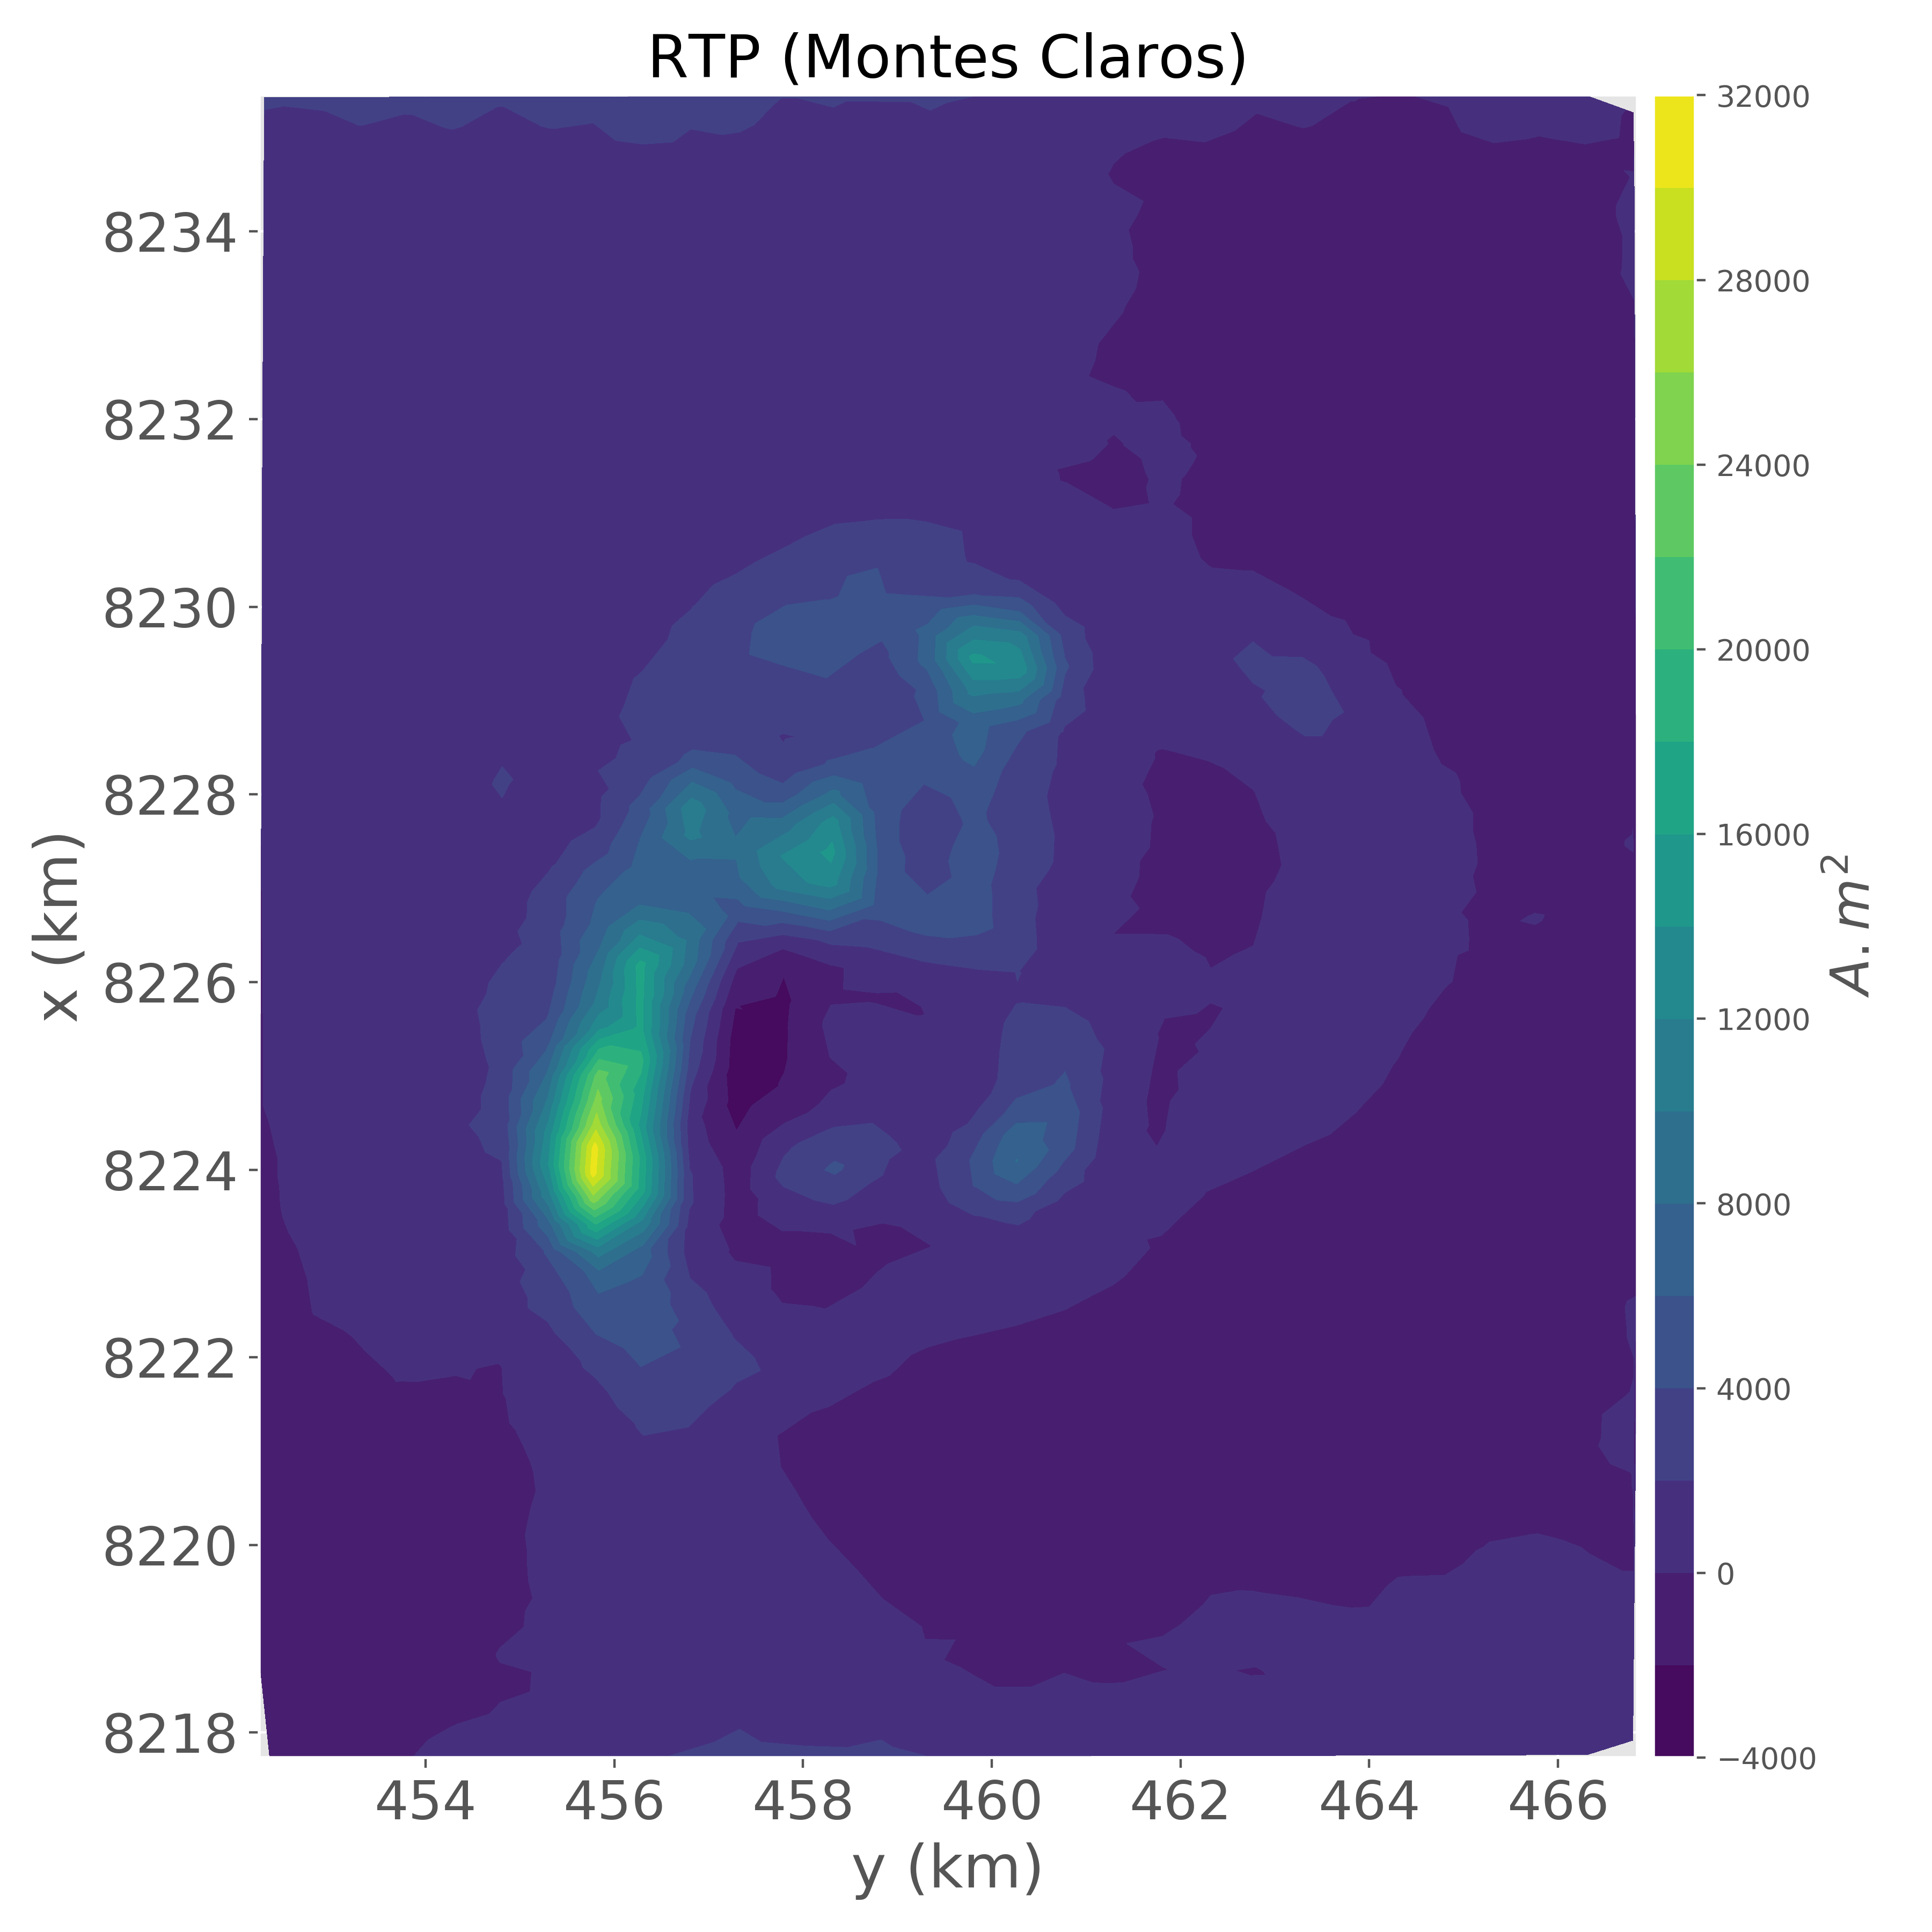
\includegraphics[width=.9\textwidth]{Fig/eqlayer/field_data_montes_claros/RTP_data_montes_claros.png}
	\caption{Redução ao polo dos dados reais do complexo de Montes Claros de Goiás (Figura \ref{fig:data_fitting_real}a) utilizando a 
	distribuição de intensidades de momentos magnéticos estimada mostrada na Figura \ref{fig:dist_momentos_pos_real}}
	\label{fig:rtp_mc_data}
\end{figure}


%%Simulações numéricas II (calculo magvec)
\chapter{Testes sintéticos para o cálculo das componentes e da amplitude do vetor magnético}
\label{chap:synt_tests_II}

Testamos a técnica da camada equivalente para o cálculo das componentes e da amplitude do vetor magnético em dois conjuntos de dados sintéticos simulando diferentes amostras de rochas. No primeiro teste, aplicamos a técnica para analisar a dependência da direção de magnetização para o cálculo das componentes e da amplitude em um modelo que representa uma amostra de rocha homogeneamente magnetizada (Seção \ref{sec:simple_sample}). No segundo, o conjunto de dados sintéticos é gerado por um modelo com mais complexidade que contém grãos fortemente magnetizados e concentrados em uma determinada região ao longo da amostra sintética de rocha (Seção \ref{sec:hetero_sample}). 

\section{Simulação de amostra simples}
\label{sec:simple_sample}

Geramos uma amostra de rocha sintética que pode simular tanto uma rocha ígnea quanto uma rocha sedimentar com intensidade de magnetização alta, considerando que a mesma seja homogeneamente magnetizada \citep{collinson1983,dunlop1997}. Com este propósito, geramos um prisma retangular de dimensões $18$ mm, $12$ mm e $2$ mm ao longo dos eixos $x$, $y$ e $z$, respectivamente. A intensidade de magnetização é igual a $1,5$ A/m. A direção de magnetização é $20^\circ$ para a inclinação e $30^\circ$ para a declinação. Os dados foram calculados em um grid regular de $100 \times 100$ pontos ao longo dos eixos $x$ e $y$, respectivamente. A distância sensor-amostra simulada foi fixada em $150$ microns acima da superfície da amostra. Por fim, os dados foram contaminados com ruído Gaussiano de média zero e desvio padrão $20$ nT. A componente vertical do campo magnético pode ser vista na figura \ref{fig:bz_homo_sample}.       

%%% Figuras teste 1
\begin{figure}
	\centering
	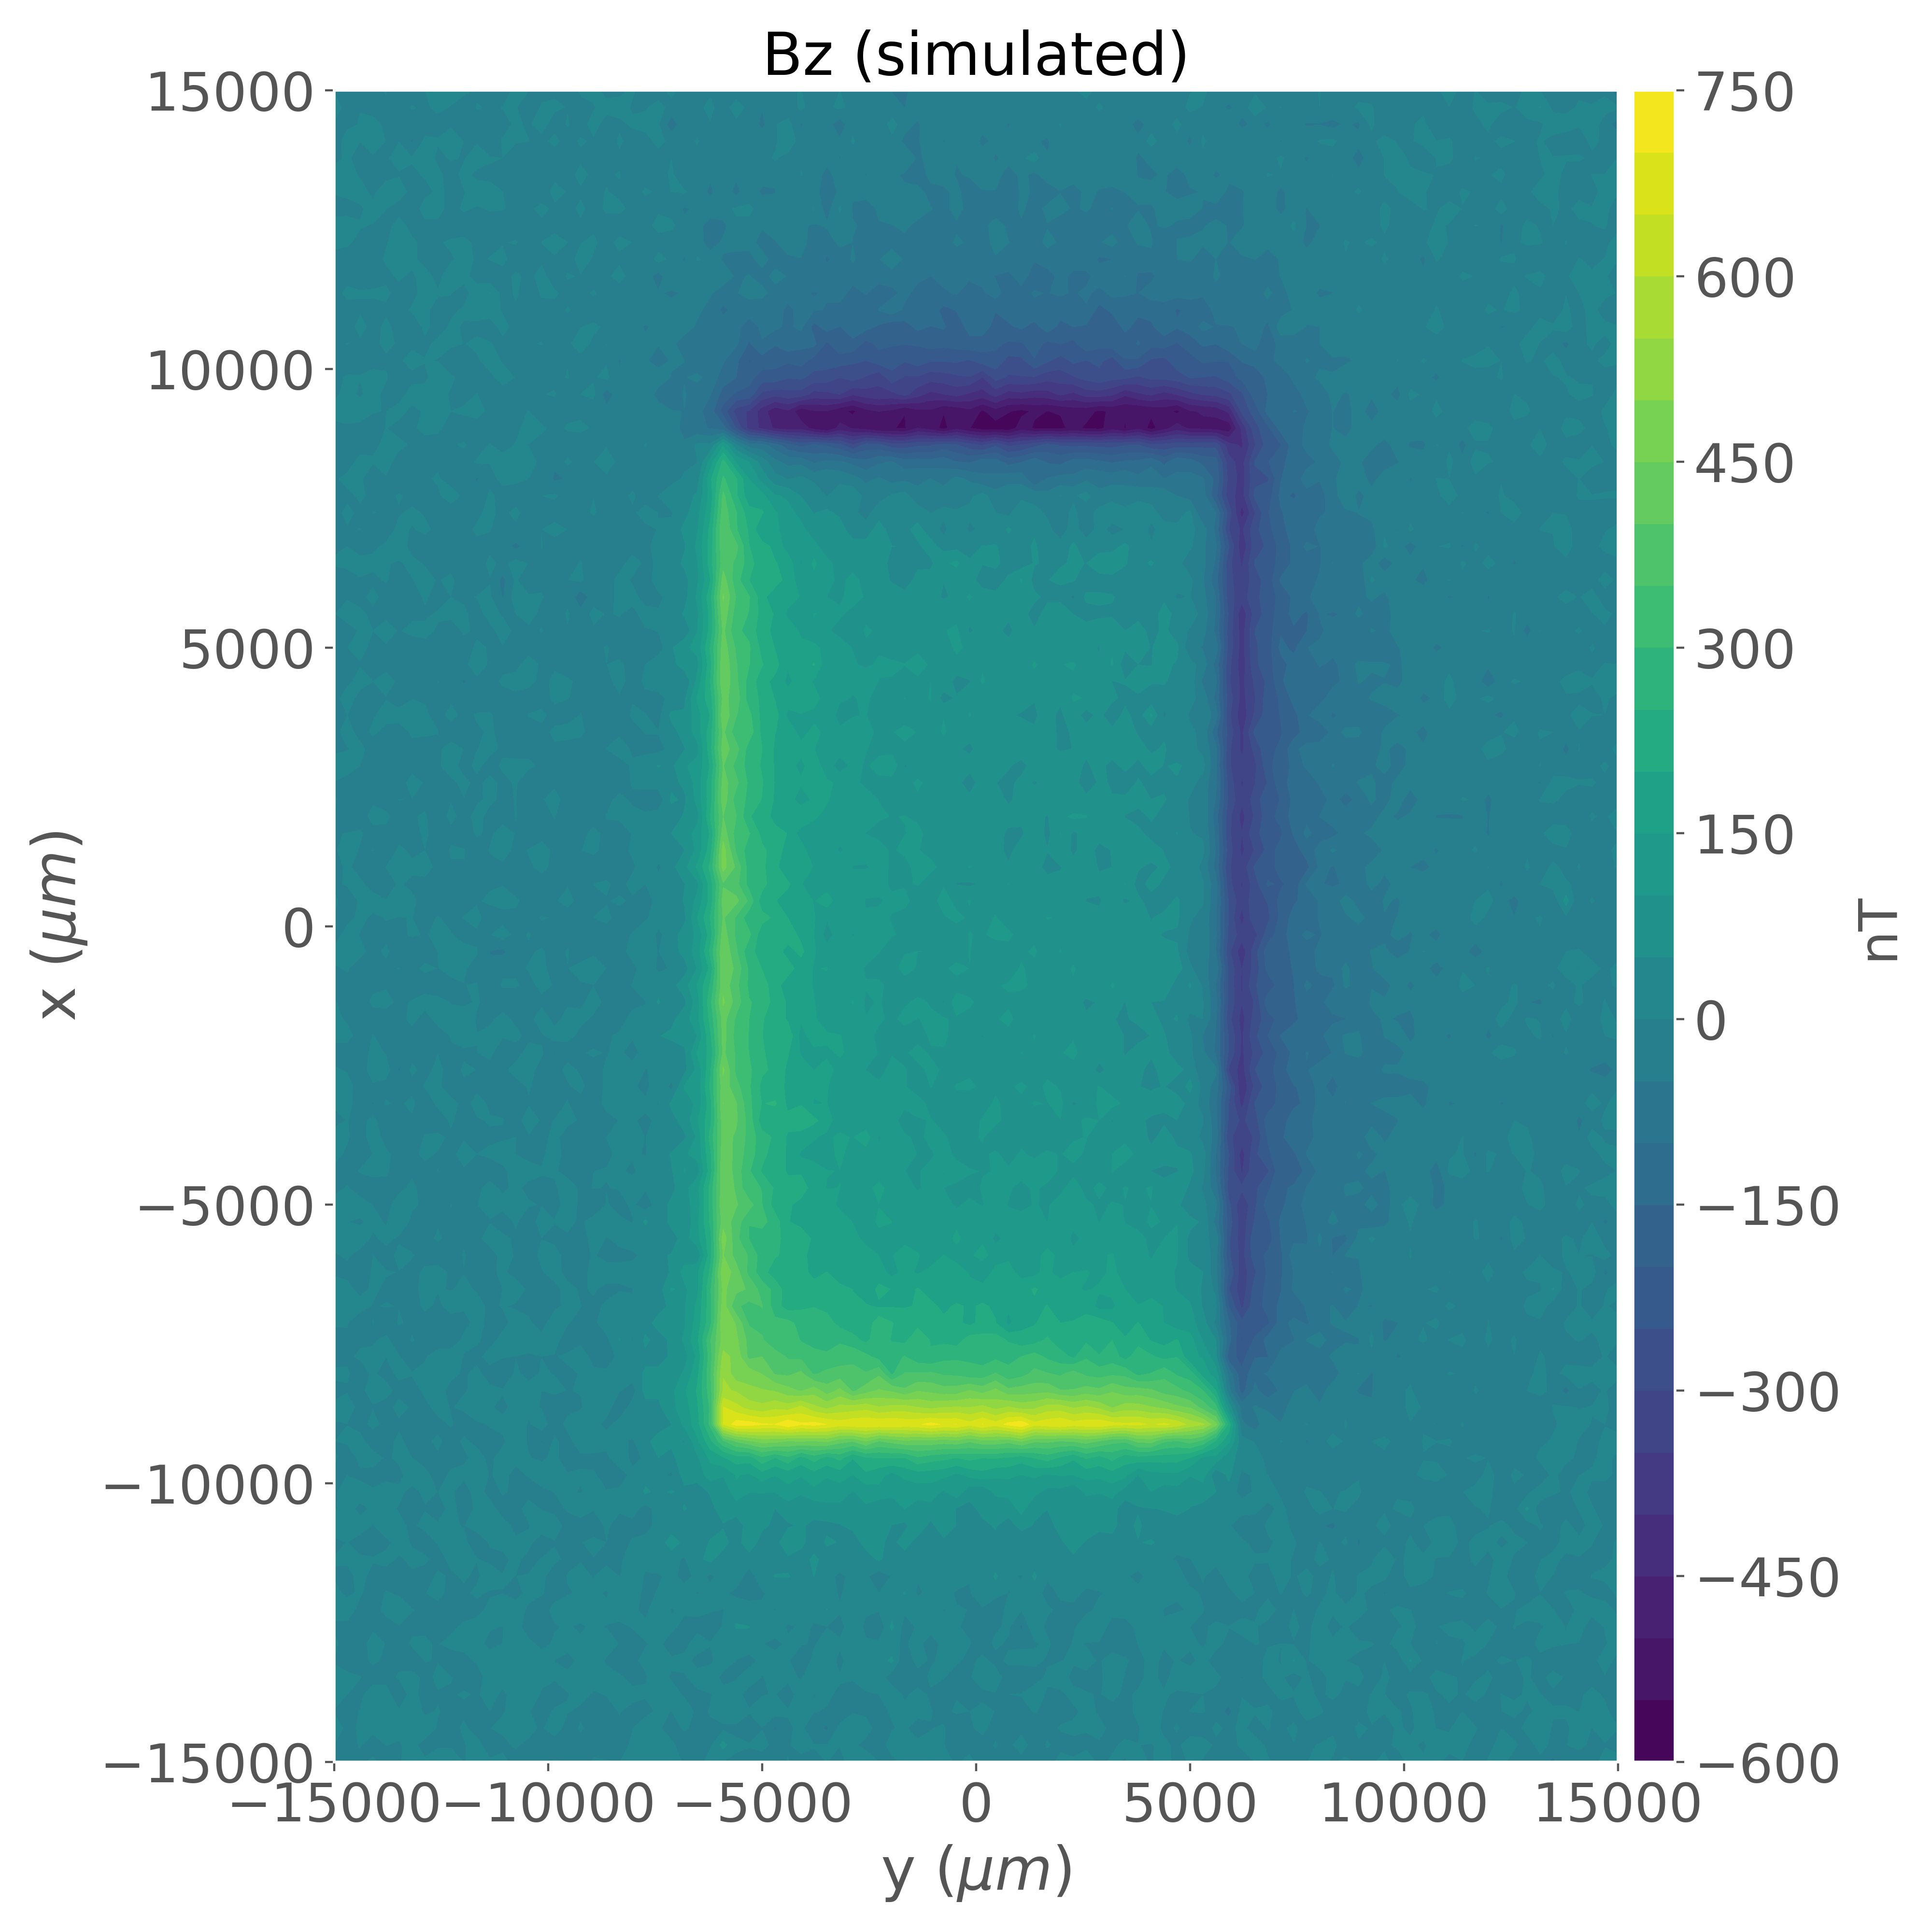
\includegraphics[width=.8\textwidth]{Fig/mag_vec/amostra_homo_correto/noisy_bz_sample.png}
	\caption{Aplicação a dados sintéticos para amostra homogeneamente magnetizada. Componente vertical do campo magnético observado contaminada com ruído Gaussiano de média zero e desvio padrão $20$ nT. A direção de magnetização é igual a $20^\circ$ para a inclinação e $30^\circ$ para a declinação. A distância sensor-amostra igual a $150$ microns. }
	\label{fig:bz_homo_sample}
\end{figure}

\subsection{Camada equivalente com a mesma direção de magnetização da amostra}
\label{subsec:homo_same_dir}

Utilizamos uma camada equivalente composta por um grid de $100 \times 100$ posicionados a uma profundidade de $z_c = 750$ microns abaixo do plano de observação. A direção de magnetização para as fontes equivalentes foi de $20^\circ$ para a inclinação e $30^\circ$ para a declinação. Utilizando a equação \ref{eq:linear_sys_p_alpha}, estimamos a distribuição de momentos magnéticos (não mostrada). A Figura \ref{fig:datafit_homo_sample_samedir}b mostra os dados preditos produzidos pela camada equivalente. A Figura \ref{fig:datafit_homo_sample_samedir}c mostra os resíduos definidos pela diferença entre os dados simulados (Figura \ref{fig:datafit_homo_sample_samedir}a) e os dados preditos (Figura \ref{fig:datafit_homo_sample_samedir}b). Os resíduos aparecem com distribuição normal de média $-0,02 \, nT$ e desvio padrão $14,36 \, nT$ como mostrado na figura \ref{fig:datafit_homo_sample_samedir}d. Com a distribuição de momentos magnéticos estimada, calculamos as componentes e a amplitude do campo magnético com as equações \ref{eq:B-alpha-pred-i}--\ref{eq:Mij-matrix-alpha} e \ref{eq:amplitude_field} (Figura \ref{fig:components_homo_sample_samedir}a-d). Com o objetivo de verificarmos se a camada equivalente produziu as componentes e a ampĺitude do campo magnético com sucesso, calculamos as componentes e a amplitude verdadeiras que são mostradas nas Figuras \ref{fig:comparison_homo_sample_samedir}a, \ref{fig:comparison_homo_sample_samedir}e e \ref{fig:comparison_homo_sample_samedir}i. As Figuras \ref{fig:comparison_homo_sample_samedir}b, \ref{fig:comparison_homo_sample_samedir}f e \ref{fig:comparison_homo_sample_samedir}j são os dados preditos pela camada equivalente, que são os mesmos dados mostrados na Figura \ref{fig:datafit_homo_sample_samedir}.
As Figuras \ref{fig:comparison_homo_sample_samedir}c, \ref{fig:comparison_homo_sample_samedir}g e \ref{fig:comparison_homo_sample_samedir}k são resíduos entre os dados verdadeiros e os dados preditos pela camada. As Figuras \ref{fig:comparison_homo_sample_samedir}d, \ref{fig:comparison_homo_sample_samedir}h e \ref{fig:comparison_homo_sample_samedir}l são os histogramas dos resíduos. Diante destes resultados, podemos concluir que as estimativas para as componentes e a amplitude do campo magnético foram excelentes, de forma que a inversão produziu dados muito próximos dos verdadeiros.  

%% Figuras 
\begin{figure}
	\centering
	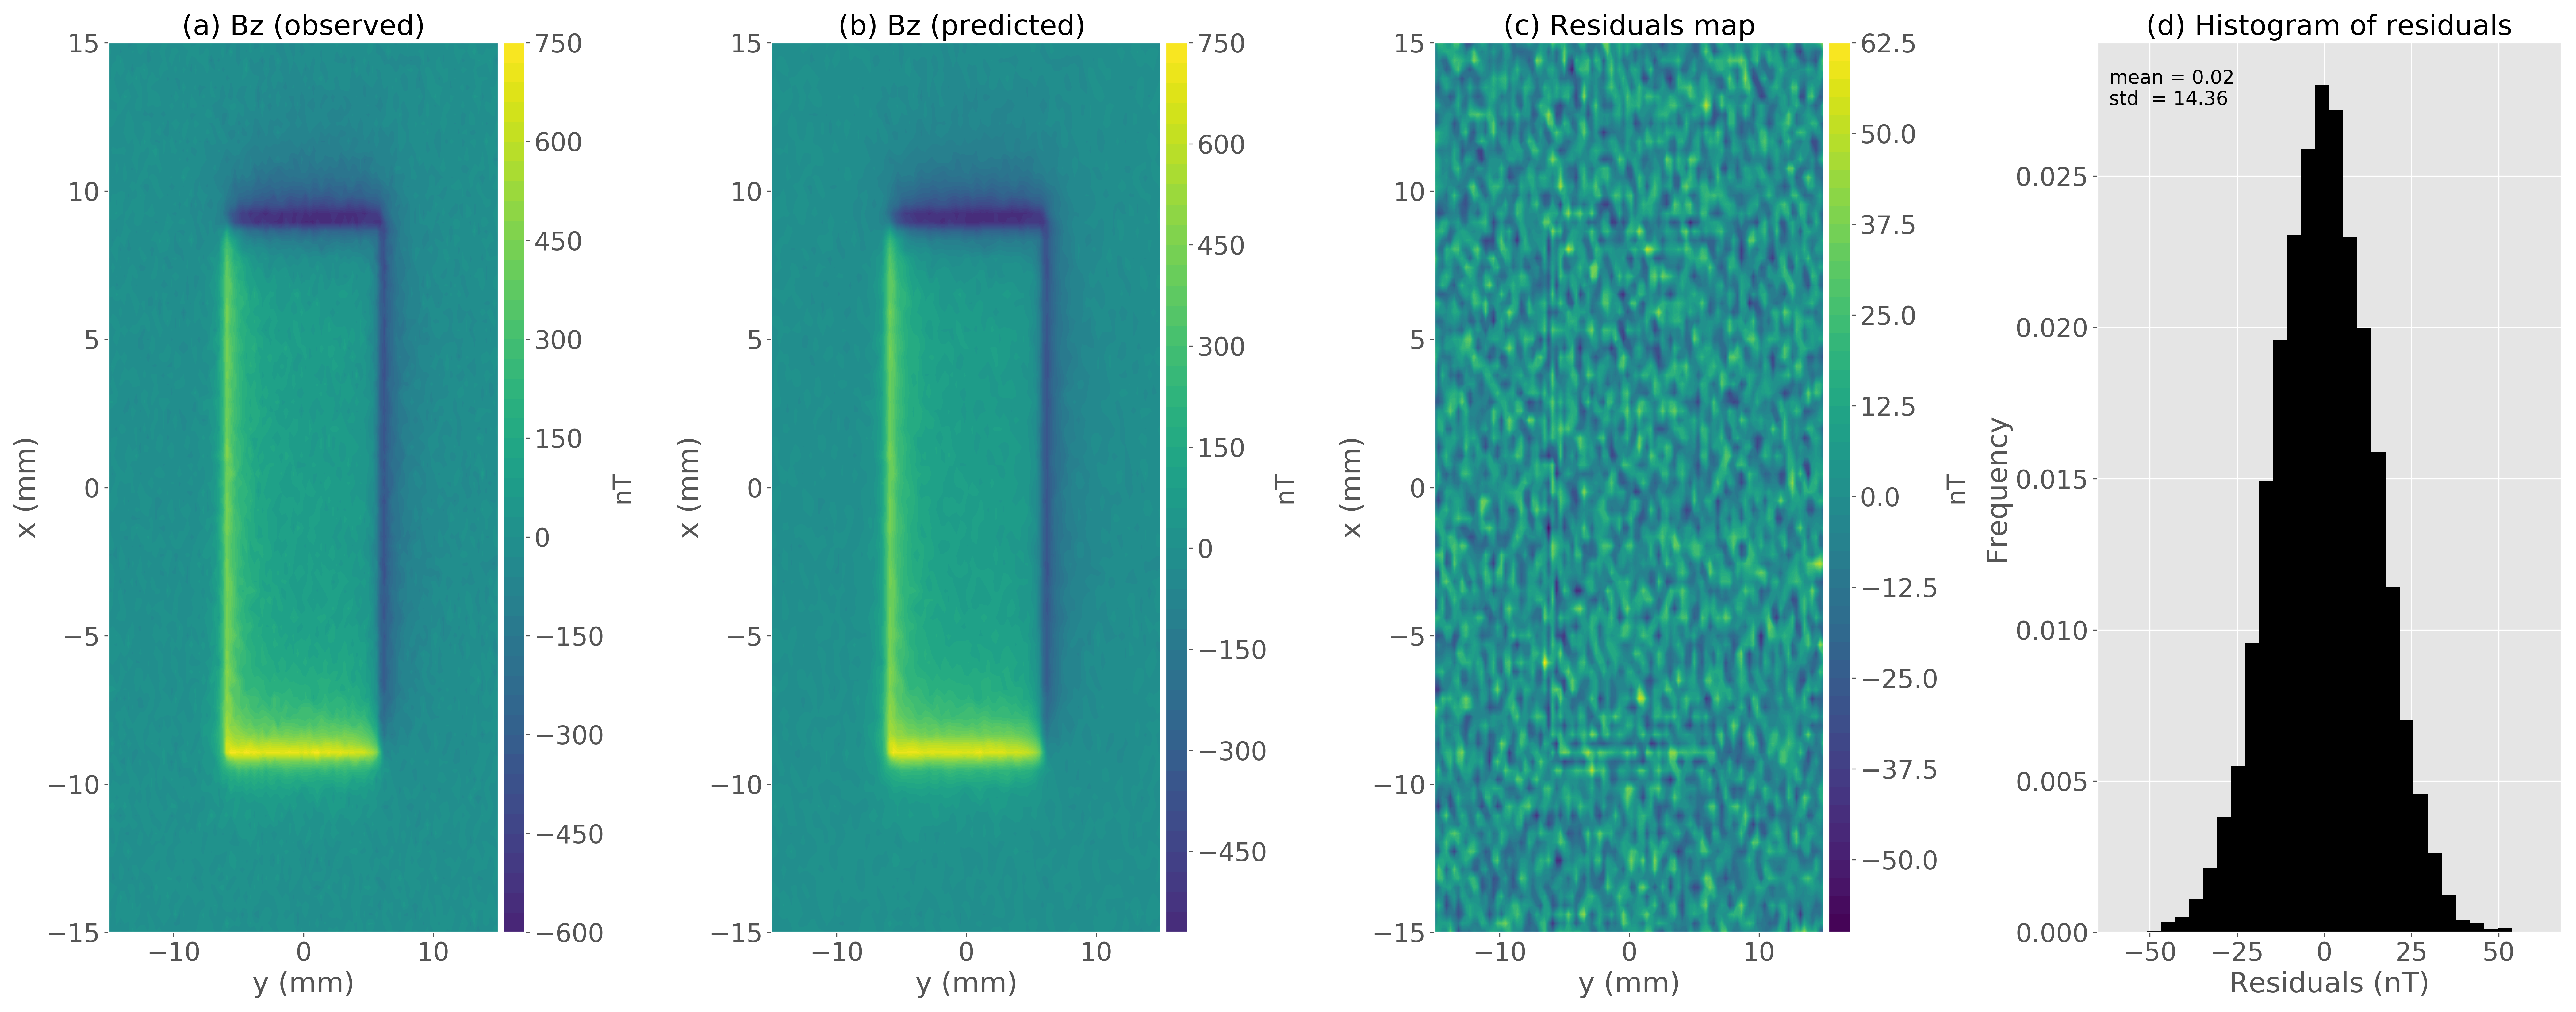
\includegraphics[width=.9\textwidth]{Fig/mag_vec/amostra_homo_correto/results_data_fitting_Bz.png}
	\caption{Aplicação a dados sintéticos para a amostra homogênea com a mesma direção de magnetização da camada equivalente. (a) Componente vertical observada. (b) Dados preditos produzido pela camada equivalente. (c) Diferença entre os dados mostrados nos gráficos a e b. (d) Histograma dos resíduos.}
	\label{fig:datafit_homo_sample_samedir}
\end{figure}

\begin{figure}
	\centering
	\includegraphics[width=1.\textwidth]{Fig/mag_vec/amostra_homo_correto/field_components_eqlayer.png}
	\caption{Aplicação a dados sintéticos para a amostra homogênea com a mesma direção de magnetização da camada equivalente. (a) Componente vertical predita pela camada. (b) Componente $x$ do campo magnético predita pela camada. (c) Componente $y$ do campo magnético predita pela camada. (d) Amplitude do campo magnético calculado através da equação \ref{eq:amplitude_field}.}
	\label{fig:components_homo_sample_samedir}
\end{figure}

\begin{figure}
	\centering
	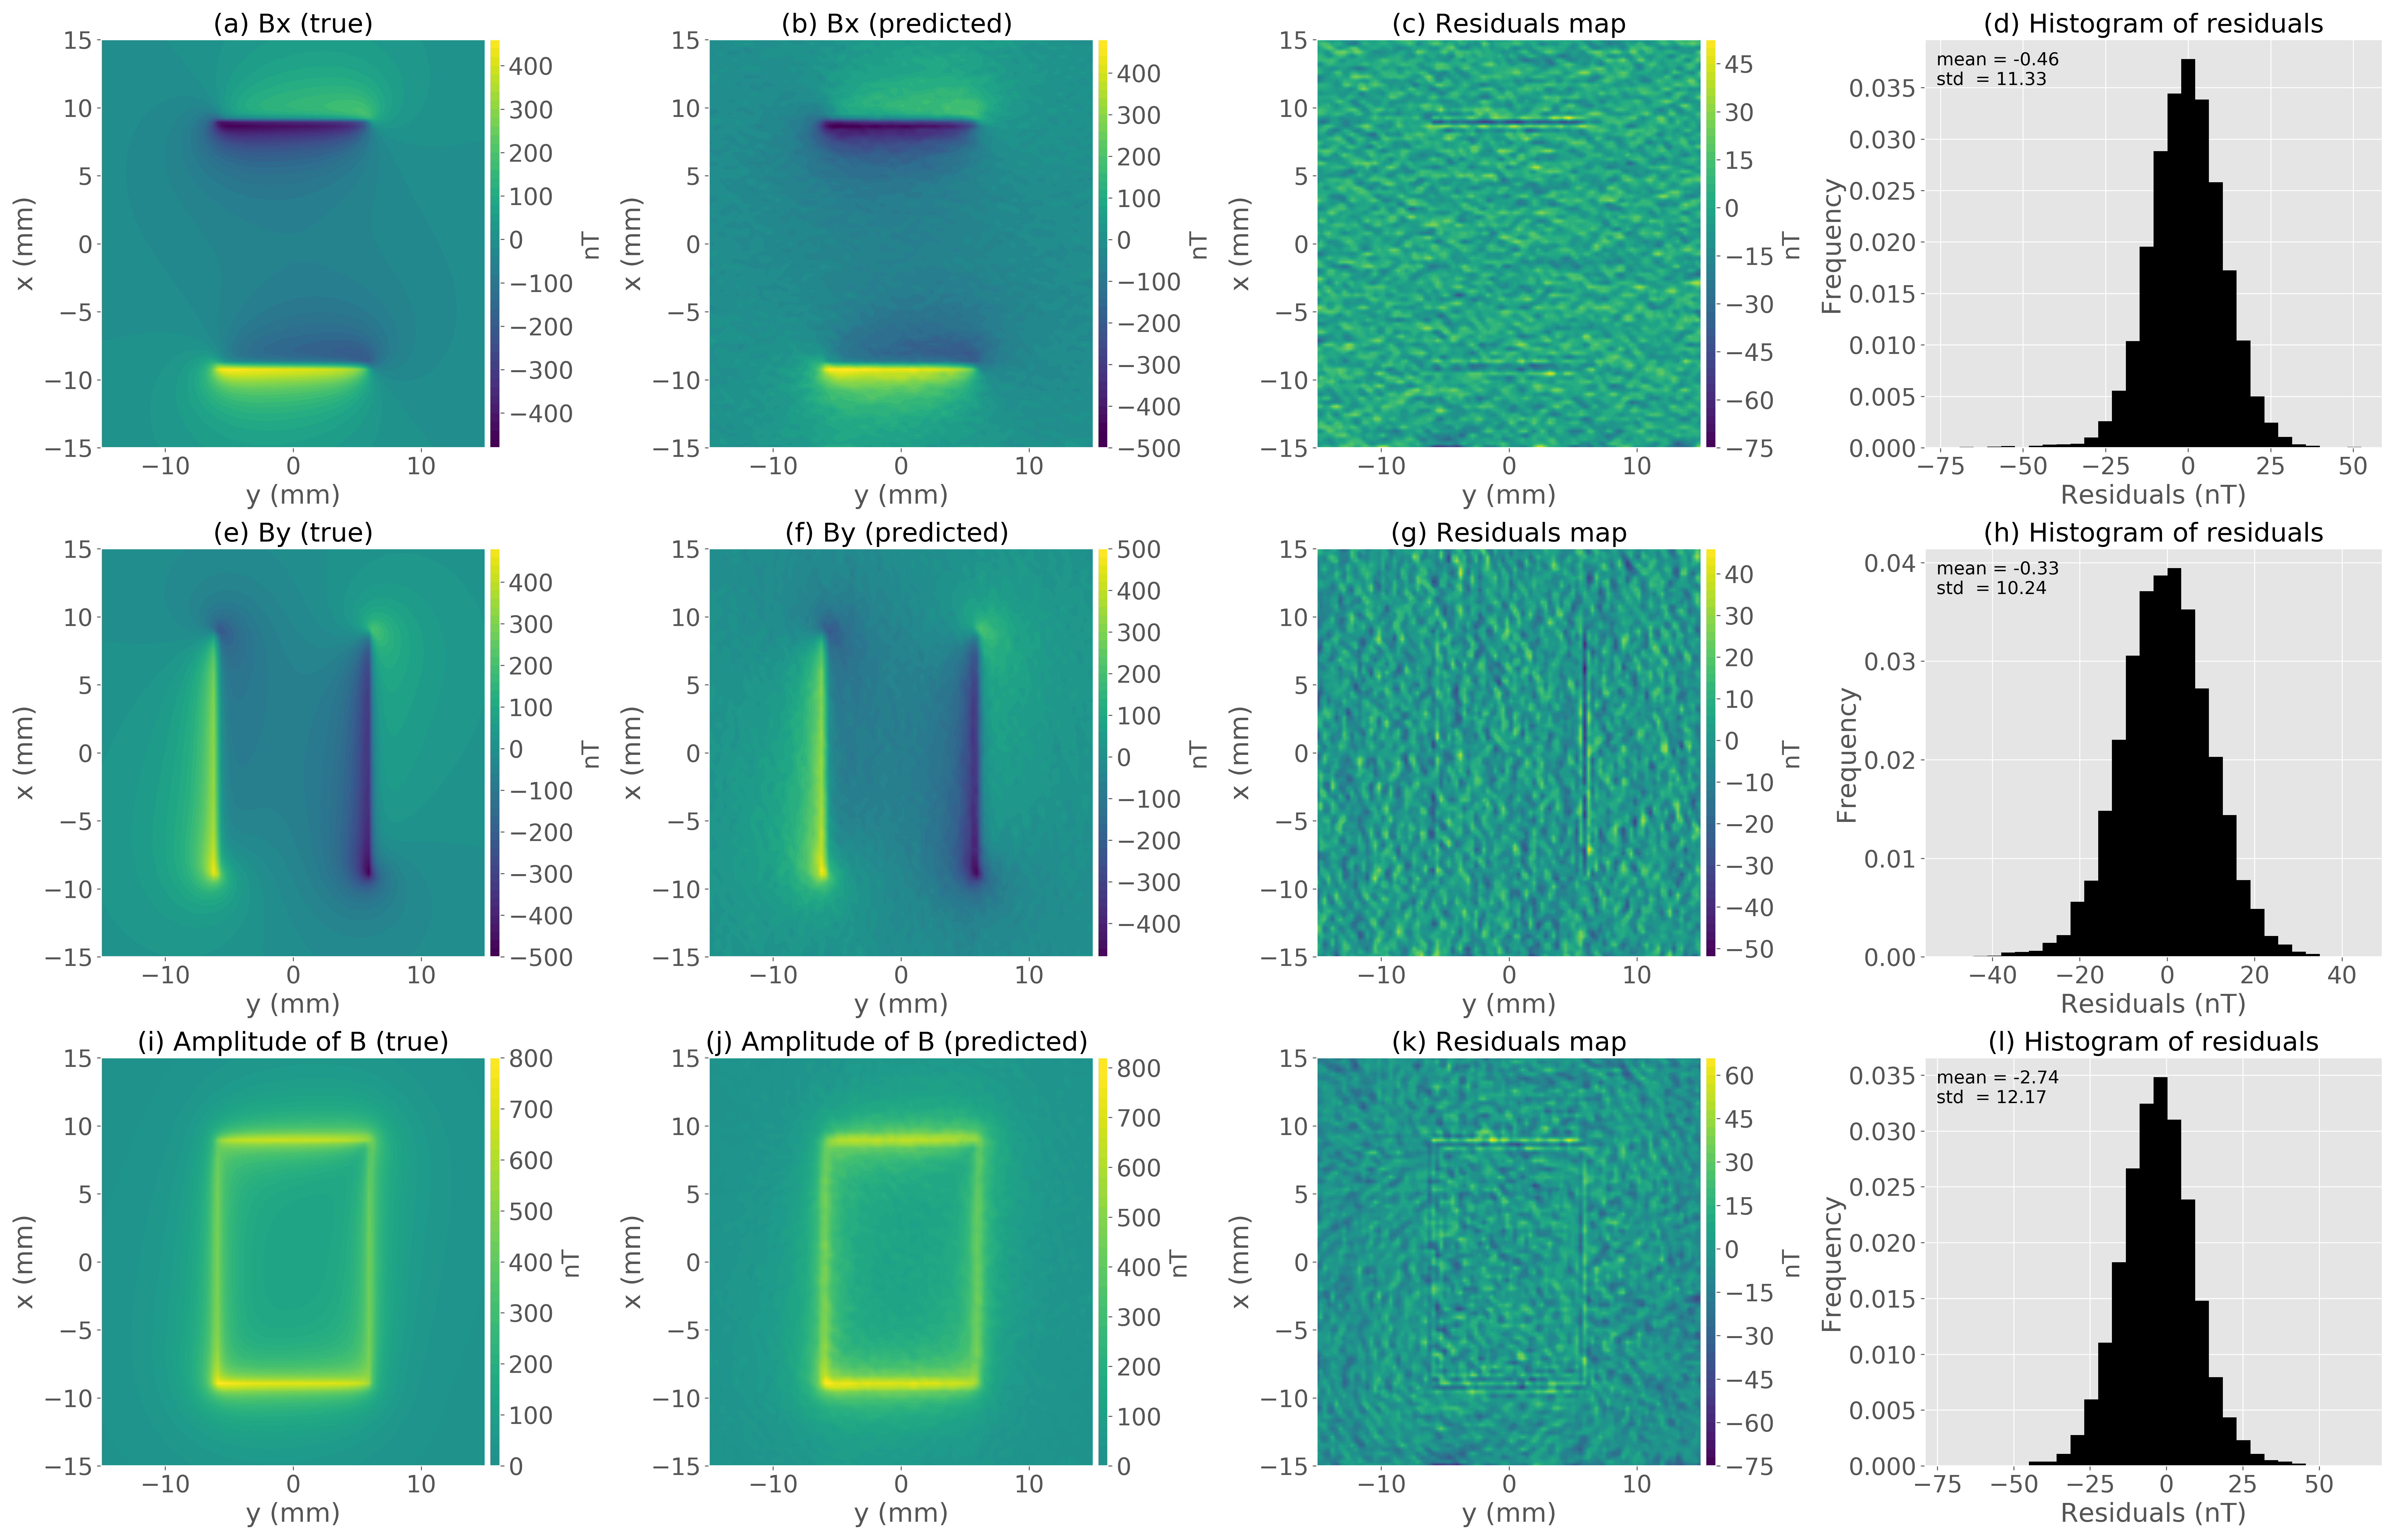
\includegraphics[width=1.15\textwidth]{Fig/mag_vec/amostra_homo_correto/comparison_true_estimated.png}
	\caption{Aplicação a dados sintéticos para a amostra homogênea com a mesma direção de magnetização da camada equivalente. (a),(e) e (i) Componentes $x$, $y$ e a amplitude verdadeiras do campo magnético, respectivamente. (b), (f) e (j) Componentes $x$, $y$ e a amplitude do campo magnético preditas pela camada equivalente, respectivamente. (c), (g) e (k) Mapas dos resíduos. (d), (h) e (l) Histograma dos resíduos.}
	\label{fig:comparison_homo_sample_samedir}
\end{figure}


\subsection{Camada equivalente com direção de magnetização diferente da amostra}
\label{subsec:homo_dif_dir}

Utilizamos uma camada equivalente composta por um grid de $100 \times 100$ posicionados a uma profundidade de $z_c = 750$ microns abaixo do plano de observação. A direção de magnetização para as fontes equivalentes foi de $50^\circ$ para a inclinação e $60^\circ$ para a declinação, enquanto a amostra possui $20^\circ$ para a inclinação e $30^\circ$ para a declinação. Utilizando a equação \ref{eq:linear_sys_p_alpha}, estimamos a distribuição de momentos magnéticos (não mostrado). A figura \ref{fig:datafit_homo_sample_difdir}b mostra os dados preditos produzidos pela camada equivalente. A figura \ref{fig:datafit_homo_sample_difdir}c mostra os resíduos definidos pela diferença entre os dados simulados (Figura \ref{fig:datafit_homo_sample_difdir}a) e os dados preditos (Figura \ref{fig:datafit_homo_sample_difdir}b). Os resíduos aparecem com distribuição normal de média $-0,02 \, nT$ e desvio padrão $15,02 \, nT$ como mostrado na figura \ref{fig:datafit_homo_sample_difdir}d. Com a distribuição de momentos magnéticos estimada, conseguimos calcular as componentes e a amplitude do campo magnético com as equações \ref{eq:B-alpha-pred-i}--\ref{eq:Mij-matrix-alpha} e \ref{eq:amplitude_field} (Figura \ref{fig:components_homo_sample_difdir}a-d). Com o objetivo de verificarmos se a camada equivalente produziu as componentes e a ampĺitude do campo magnético com sucesso, calculamos os valores verdadeiros que são mostrados nas  figuras \ref{fig:comparison_homo_sample_difdir}a, \ref{fig:comparison_homo_sample_difdir}e e \ref{fig:comparison_homo_sample_difdir}i. As Figuras \ref{fig:comparison_homo_sample_difdir}b, \ref{fig:comparison_homo_sample_difdir}f e \ref{fig:comparison_homo_sample_difdir}j são os dados preditos pela camada equivalente. As Figuras \ref{fig:comparison_homo_sample_difdir}c, \ref{fig:comparison_homo_sample_difdir}g e \ref{fig:comparison_homo_sample_difdir}k são resíduos entre os dados verdadeiros e os dados preditos pela camada. As Figuras \ref{fig:comparison_homo_sample_difdir}d, \ref{fig:comparison_homo_sample_difdir}h e \ref{fig:comparison_homo_sample_difdir}l são os histogramas dos resíduos. Os resultados mostram que apesar da camada equivalente ter direção de magnetização muito diferente da direção da amostra, as estimativas para as componentes e a amplitude do campo magnético foram aceitáveis.  

%%% Figuras 

\begin{figure}
	\centering
	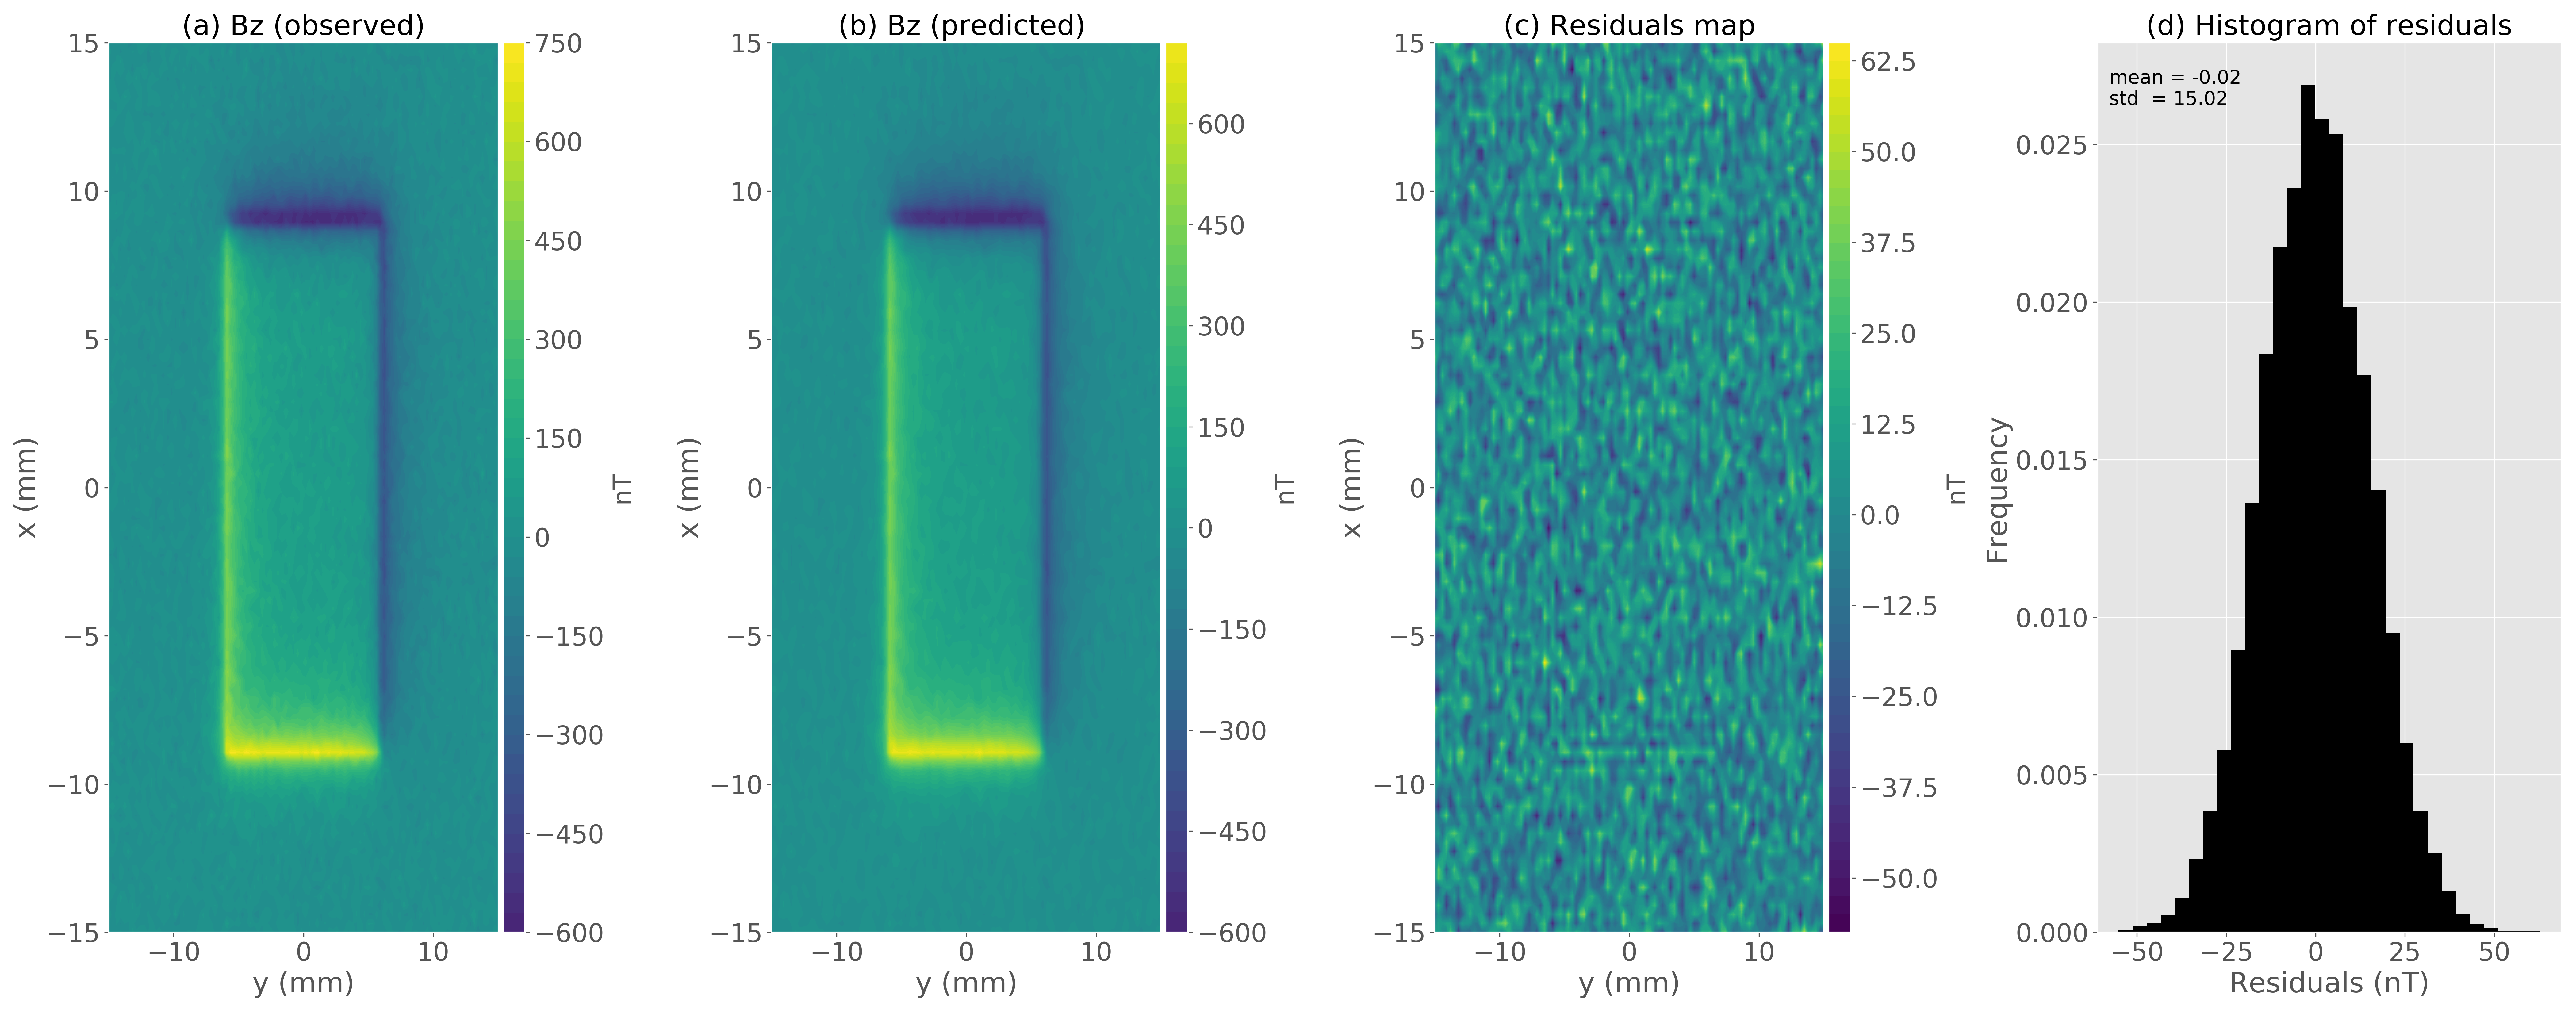
\includegraphics[width=.9\textwidth]{Fig/mag_vec/amostra_homo_errado/results_data_fitting_Bz.png}
	\caption{Aplicação a dados sintéticos para a amostra homogênea com direção de magnetização diferente da camada equivalente. (a) Componente vertical observada. (b) Dados preditos produzido pela camada equivalente. (c) Diferença entre os dados mostrados nos gráficos a e b. (d) Histograma dos resíduos.}
	\label{fig:datafit_homo_sample_difdir}
\end{figure}

\begin{figure}
	\centering
	\includegraphics[width=1.\textwidth]{Fig/mag_vec/amostra_homo_errado/field_components_eqlayer.png}
	\caption{Aplicação a dados sintéticos para a amostra homogênea com direção de magnetização diferente da camada equivalente. (a) Componente vertical predita pela camada. (b) Componente $x$ do campo magnético predita pela camada. (c) Componente $y$ do campo magnético predita pela camada. (d) Amplitude do campo magnético calculado através da equação \ref{eq:amplitude_field}.}
	\label{fig:components_homo_sample_difdir}
\end{figure}

\begin{figure}
	\centering
	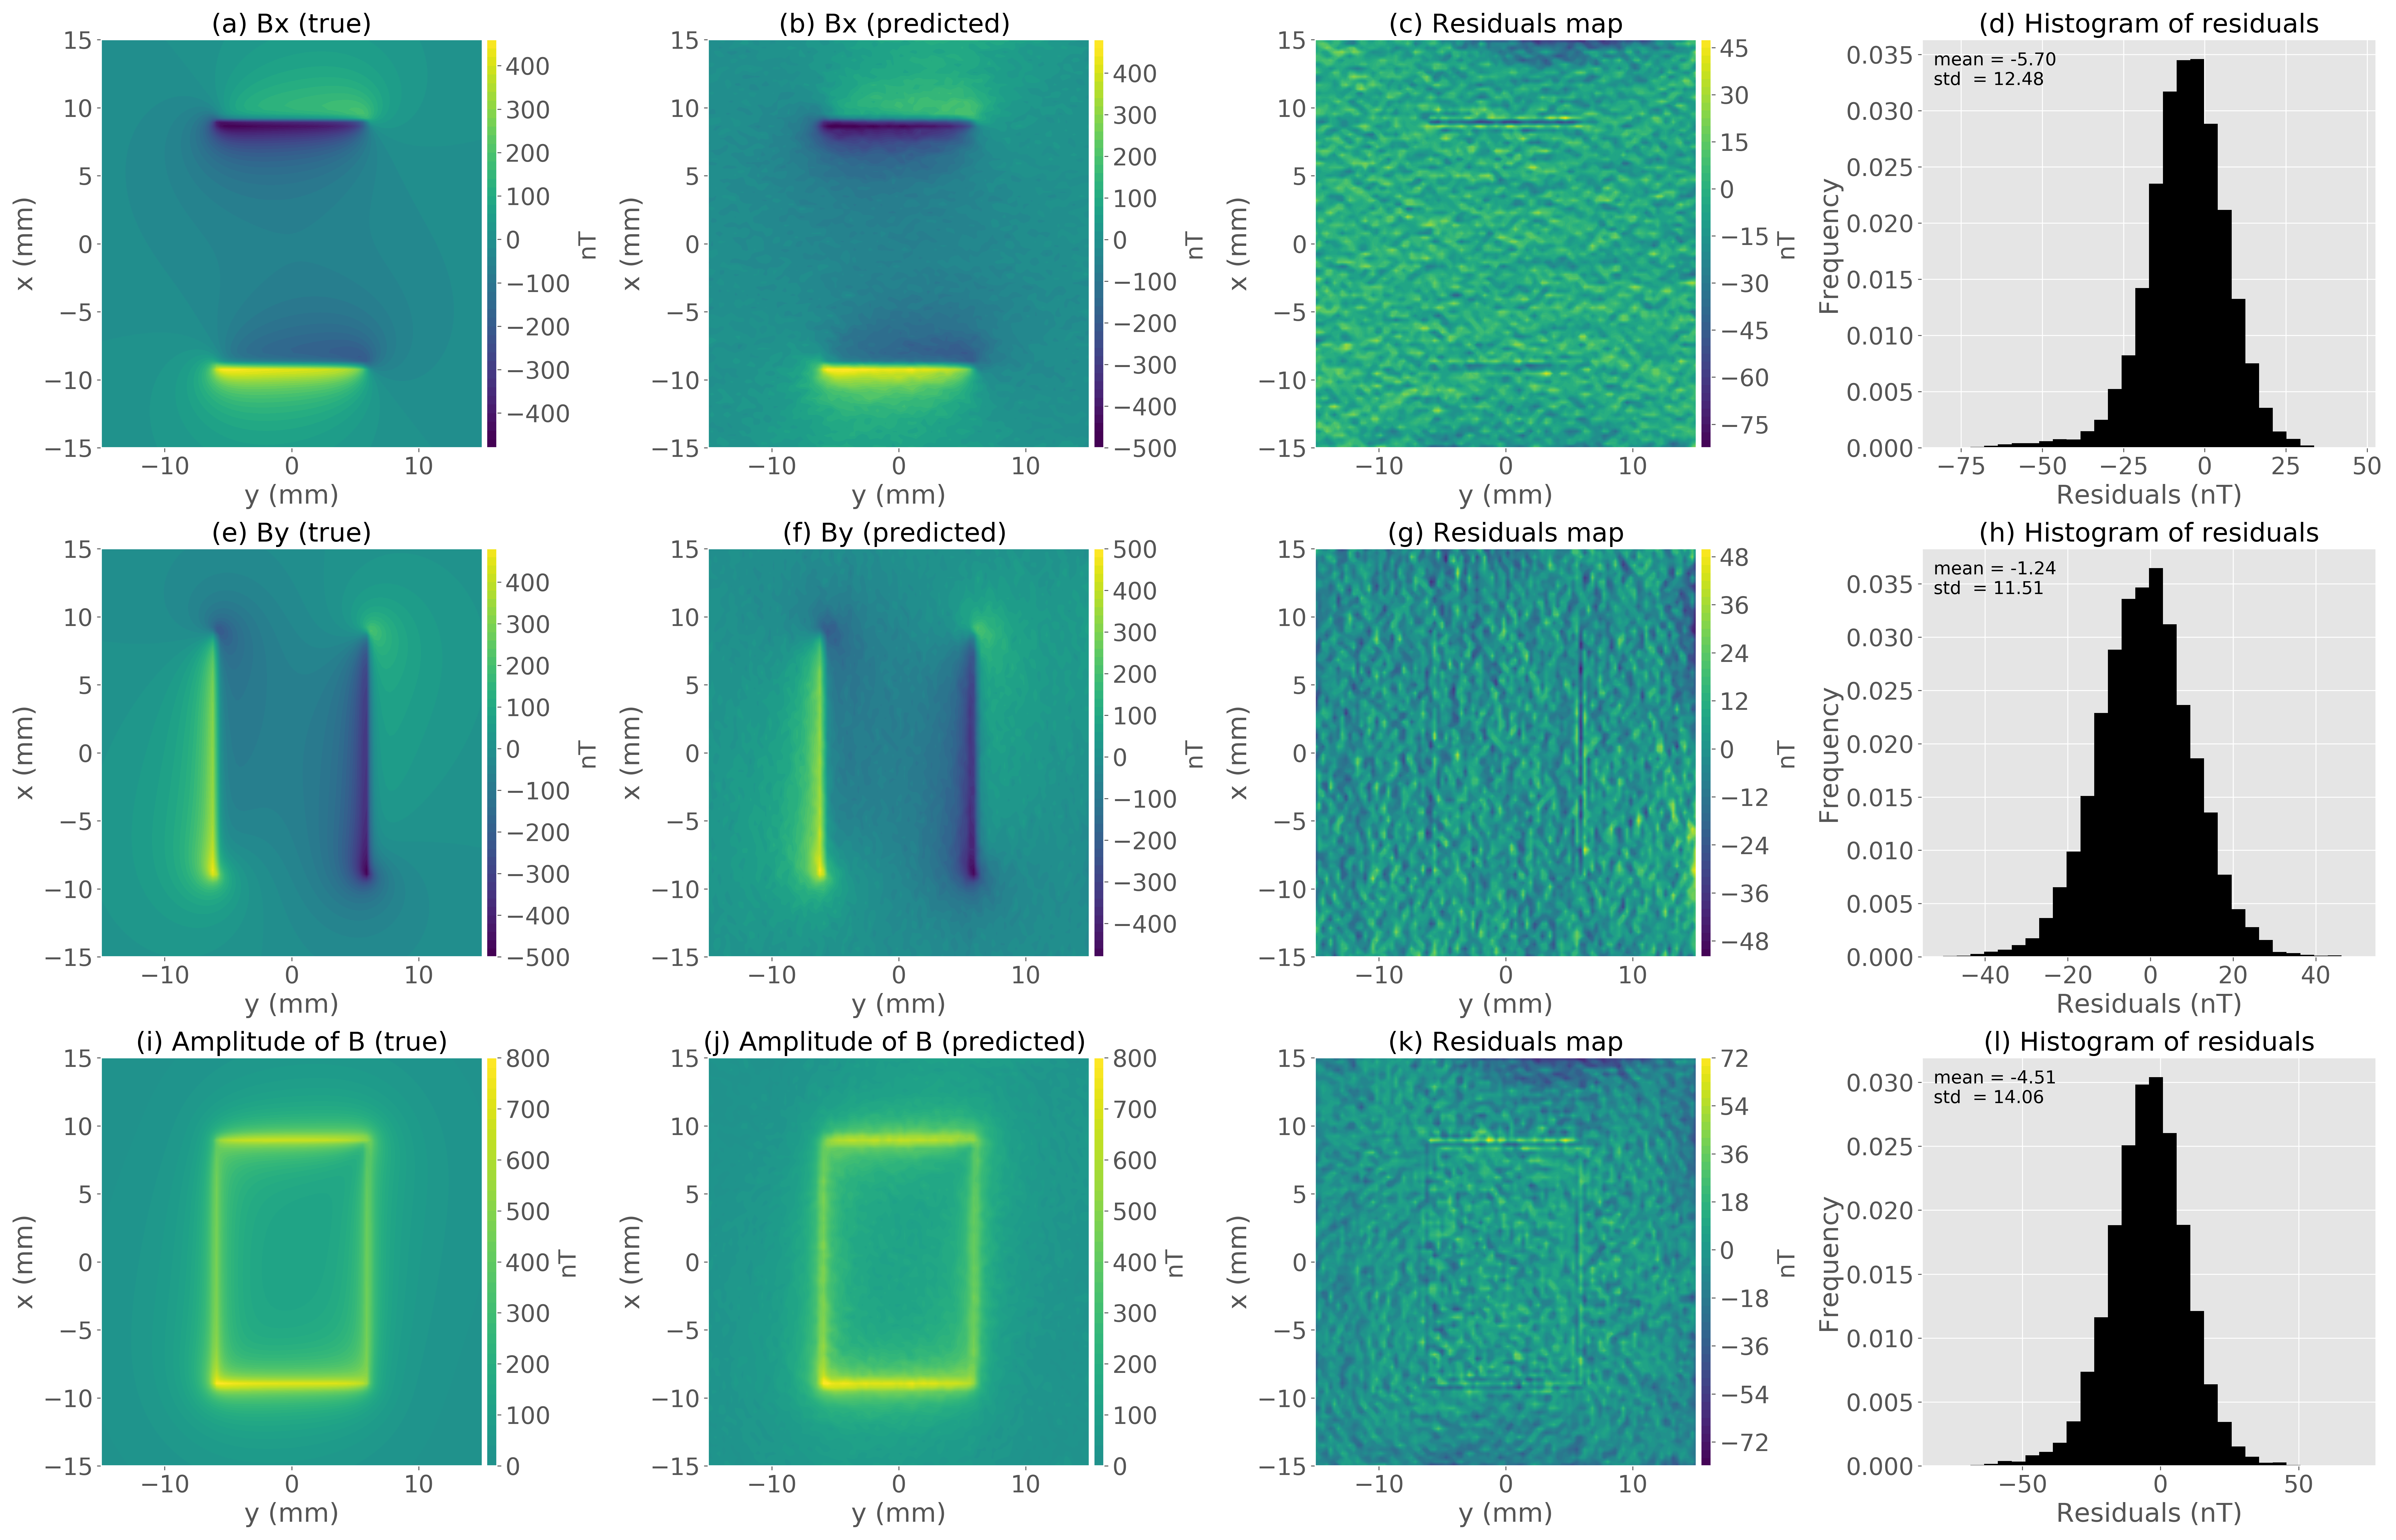
\includegraphics[width=1.15\textwidth]{Fig/mag_vec/amostra_homo_errado/comparison_true_estimated.png}
	\caption{Aplicação a dados sintéticos para a amostra homogênea com direção de magnetização diferente da camada equivalente. (a),(e) e (i) Componentes $x$, $y$ e a amplitude verdadeiras do campo magnético, respectivamente. (b), (f) e (j) Componentes $x$, $y$ e a amplitude do campo magnético preditas pela camada equivalente, respectivamente. (c), (g) e (k) Mapas dos resíduos. (d), (h) e (l) Histograma dos resíduos.}
	\label{fig:comparison_homo_sample_difdir}
\end{figure}


%%%%%%%%%%%%%%%%%%%%%%%%%%%%%%%%%%%%%%%%%%%%%%%%%%%%%%%%%%%%%%%%%%%%%%%%%%%%%%%%
\section{Simulação de amostra com heterogeneidades}
\label{sec:hetero_sample}

Neste segundo teste, geramos uma amostra de rocha sintética que possui uma distribuição de magnetização mais complexa que no caso anterior. A geometria desta amostra é dada por um prisma poligonal com espessura igual a $2,5$ mm. A intensidade de magnetização é igual a $1,5$ A/m. A direção de magnetização é igual a $90^\circ$ para inclinação e $0^\circ$ para a declinação. Além disso, adicionamos $300$ dipolos de raio igual a $100$ microns e intensidade de magnetização $500$ A/m dispostos aleatoriamente em uma determinada região da amostra, e possuem a mesma direção de magnetização do prisma poligonal. Este conjunto de dipolos representam grãos multidomínio (MD) que podem sem encontrados em rochas ígneas e sedimentares \citep{dunlop1997,butler1998,clark1997}. Os dados foram calculados em um grid regular de $121 \times 99$ ao longo dos eixos $x$ e $y$, respectivamente. A distância sensor-amostra é igual a $138$ microns acima da superfície da amostra. Simulamos um ruído Gaussiano de média zero e desvio padrão de $20$ nT. A componente vertical do campo magnético calculada é mostrada na Figura 
\ref{fig:bz_hetero_sample}.

%%%% Figuras teste 2
\begin{figure}
	\centering
	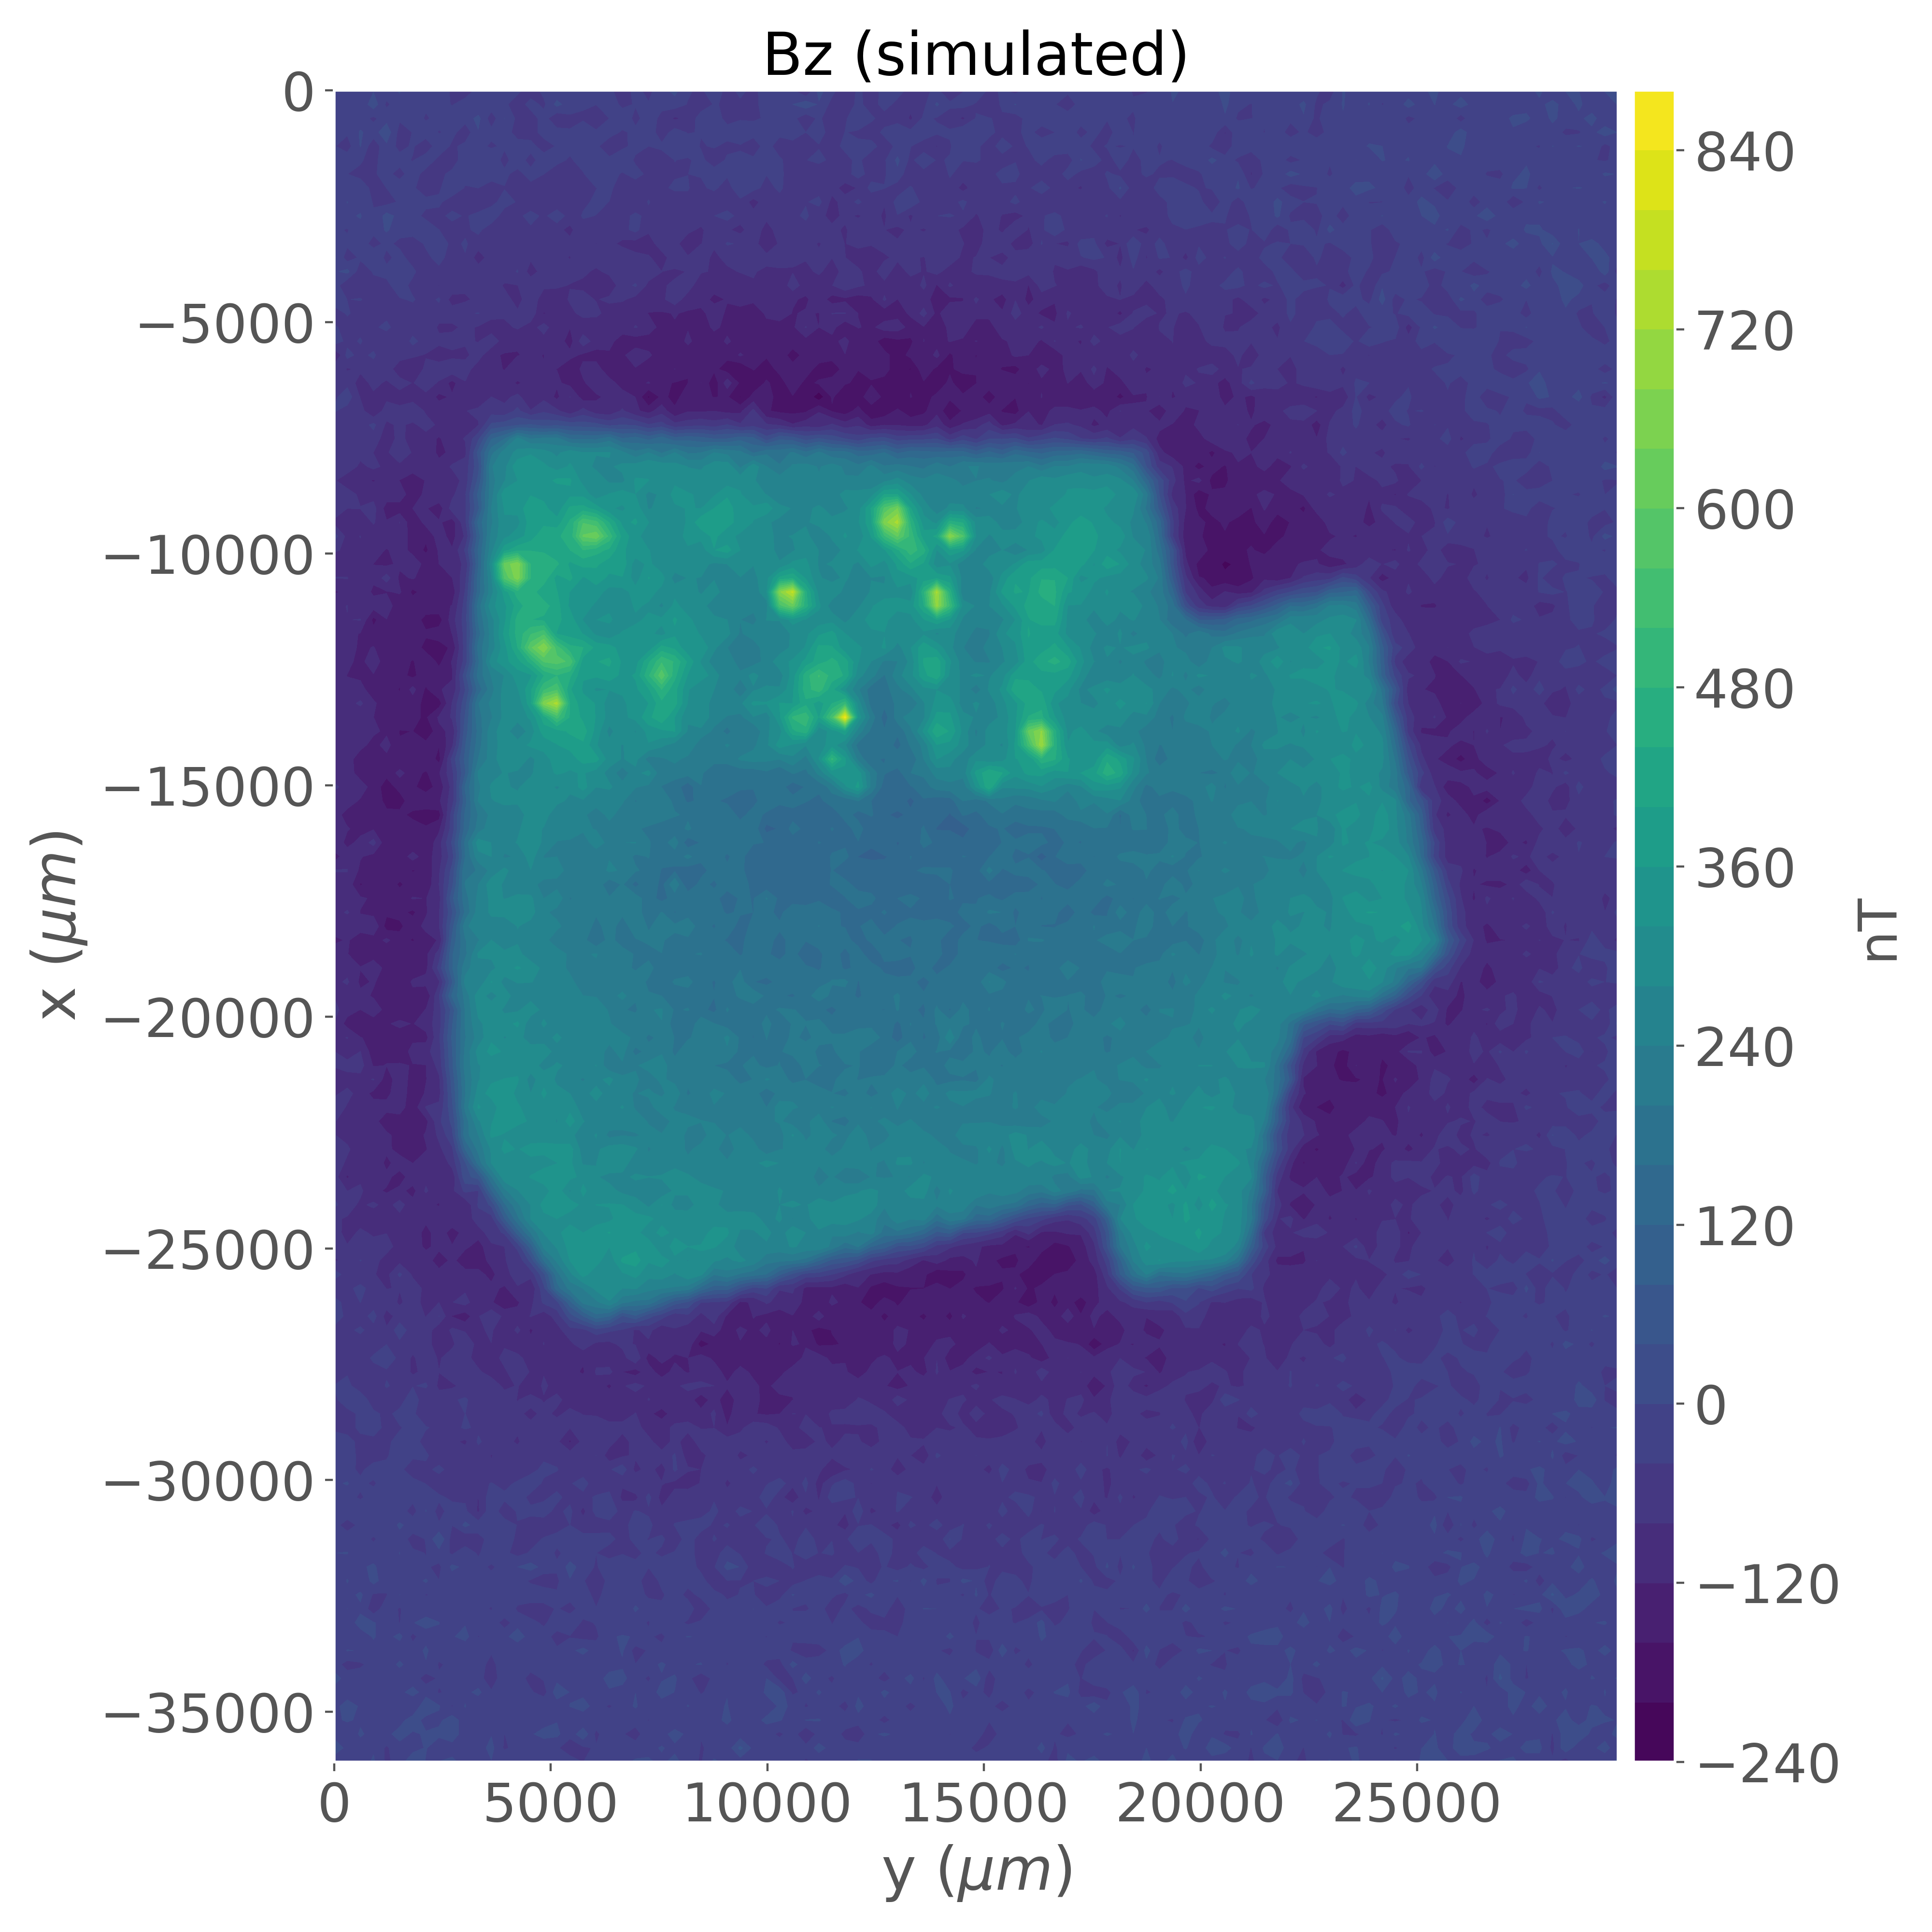
\includegraphics[width=.8\textwidth]{Fig/mag_vec/simulacao_real_correto/noisy_bz_sample.png}
	\caption{Componente vertical do campo magnético observado contaminada com ruído Gaussiano de média zero e desvio padrão $20$ nT para a amostra heterogênea. A direção de magnetização é igual a $90^\circ$ para a inclinação e $0^\circ$ para a declinação. A distância sensor-amostra igual a $138$ microns. }
	\label{fig:bz_hetero_sample}
\end{figure}


\subsection{Camada equivalente com a mesma direção de magnetização da amostra}
\label{subsec:hetero_same_dir}

Utilizamos uma camada equivalente composta por um grid de $121 \times 99$ posicionados a uma profundidade de $z_c = 868$ microns abaixo do plano de observação. A direção de magnetização para as fontes equivalentes foi de $90^\circ$ para a inclinação e $0^\circ$ para a declinação, a mesma da amostra. 
Utilizando a equação \ref{eq:linear_sys_p_alpha}, estimamos a distribuição de momentos magnéticos (não mostrado). A Figura \ref{fig:datafit_hetero_sample_samedir}b mostra os dados preditos produzidos pela camada equivalente. A Figura \ref{fig:datafit_hetero_sample_samedir}c mostra os resíduos definidos pela diferença entre os dados simulados (Figura \ref{fig:datafit_hetero_sample_samedir}a) e os dados preditos (Figura \ref{fig:datafit_hetero_sample_samedir}b). Os resíduos aparecem com distribuição normal de média $-0,09 \, nT$ e desvio padrão $16,79 \, nT$ como mostrado na figura \ref{fig:datafit_hetero_sample_samedir}d. Com a distribuição de momentos magnéticos estimada, conseguimos calcular as componentes e a amplitude do campo magnético com as equações \ref{eq:B-alpha-pred-i}--\ref{eq:Mij-matrix-alpha} e \ref{eq:amplitude_field} (Figura \ref{fig:components_hetero_sample_samedir}a-d). Com o objetivo de verificarmos se a camada equivalente produziu as componentes e a ampĺitude do campo magnético com sucesso, calculamos os valores verdadeiros que são mostrados nas  figuras \ref{fig:comparison_hetero_sample_samedir}a, \ref{fig:comparison_hetero_sample_samedir}e e \ref{fig:comparison_hetero_sample_samedir}i. As figuras \ref{fig:comparison_hetero_sample_samedir}b, \ref{fig:comparison_hetero_sample_samedir}f e \ref{fig:comparison_hetero_sample_samedir}j são os dados preditos pela camada equivalente. As figuras \ref{fig:comparison_hetero_sample_samedir}c, \ref{fig:comparison_hetero_sample_samedir}g e \ref{fig:comparison_hetero_sample_samedir}k são resíduos entre os dados verdadeiros e os dados preditos pela camada. As figuras \ref{fig:comparison_hetero_sample_samedir}d, \ref{fig:comparison_hetero_sample_samedir}h e \ref{fig:comparison_hetero_sample_samedir}l são os histogramas dos resíduos. Embora exista a influência de dipolos interferentes, as estimativas para as componentes e a amplitude do campo magnético foram aceitáveis. Portanto, a estimativa do conjunto de momentos magnéticos produziu um bom ajuste dos dados.   

%%% Figuras 

\begin{figure}
	\centering
	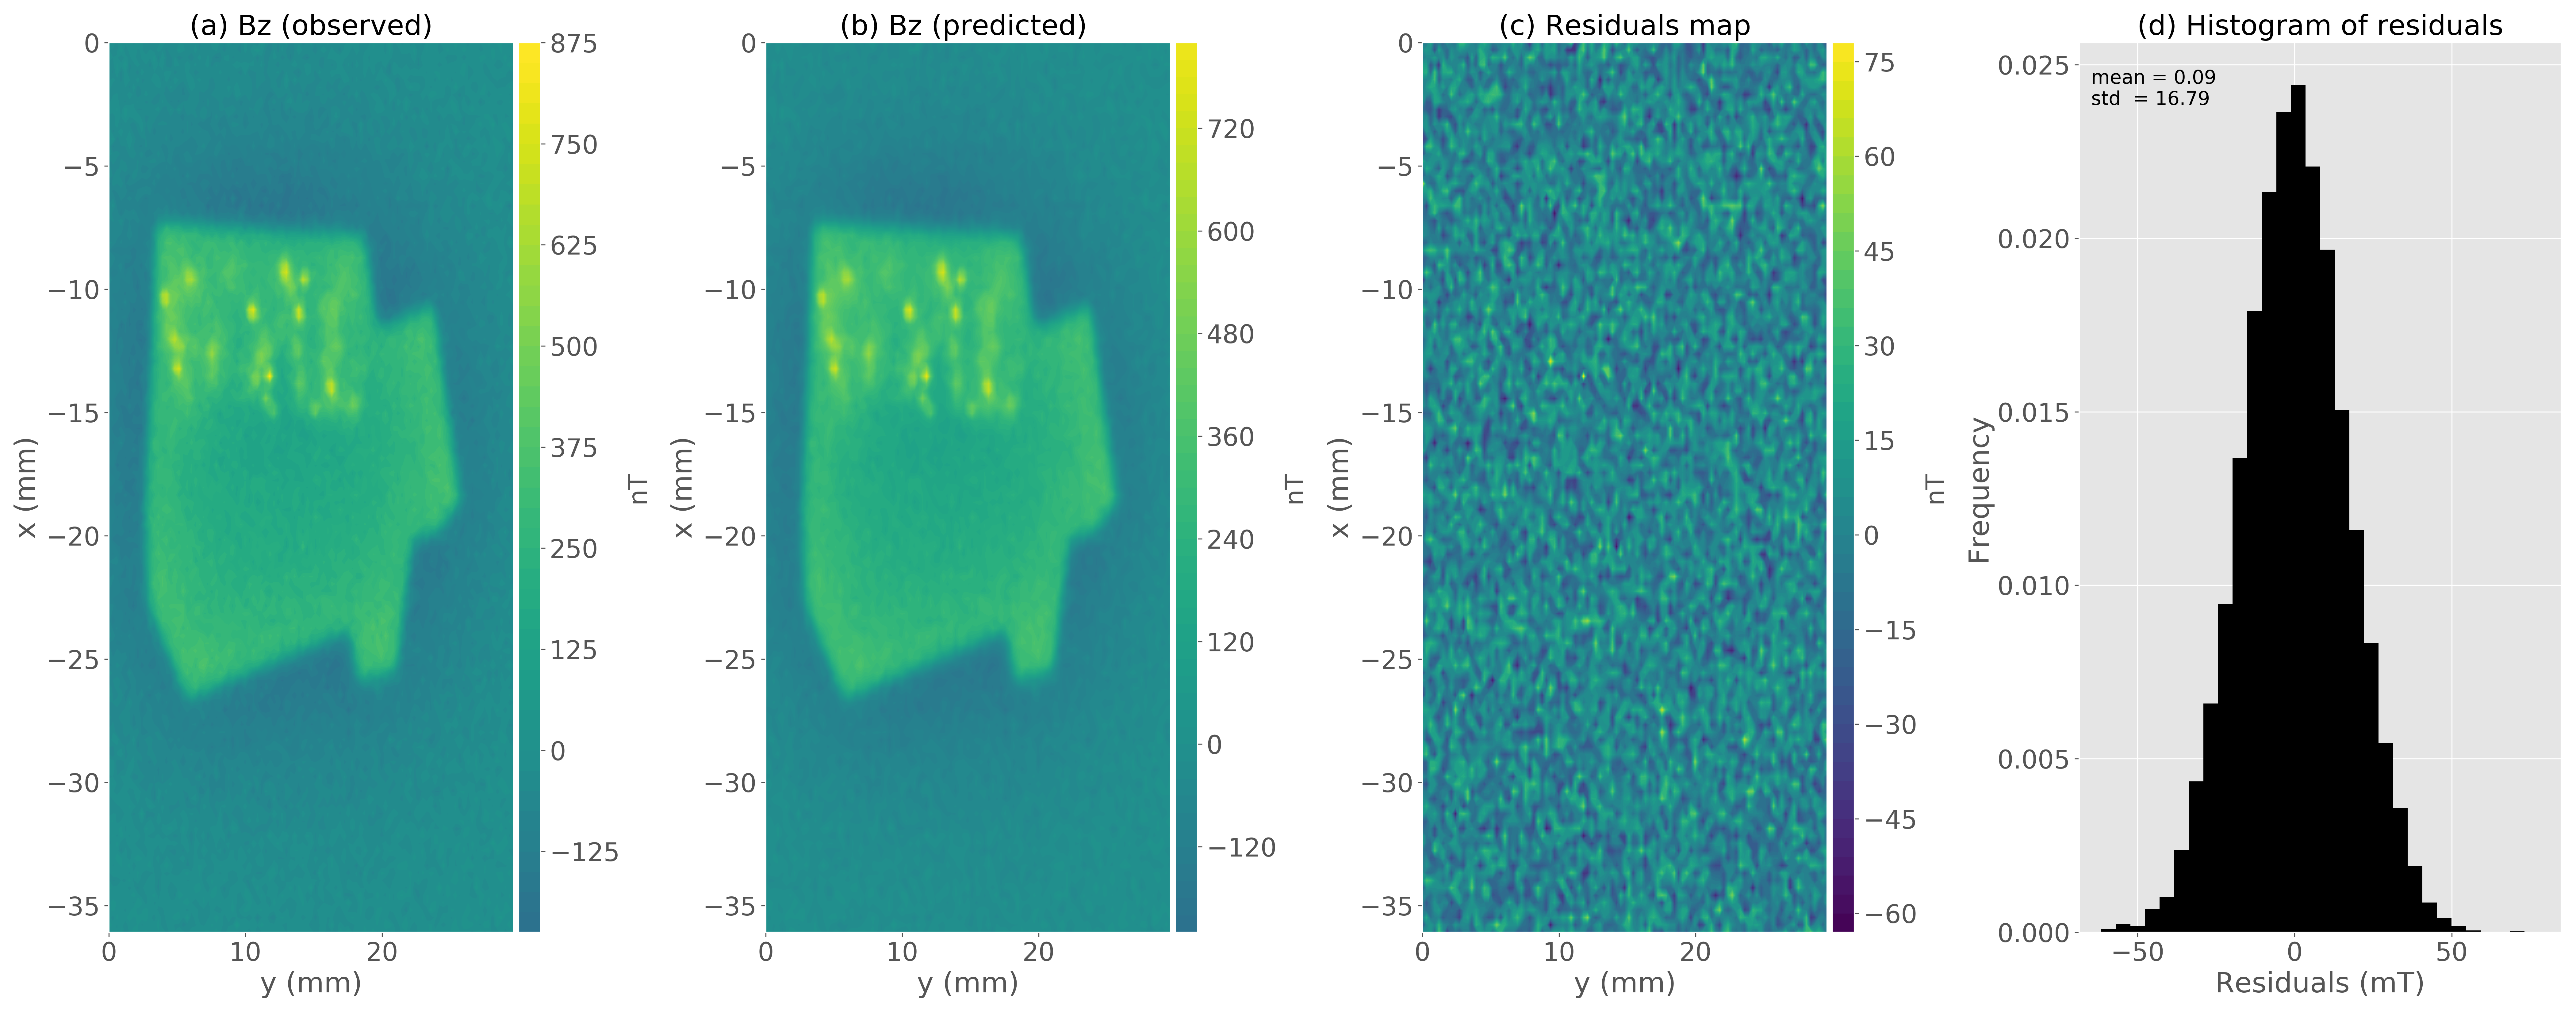
\includegraphics[width=.9\textwidth]{Fig/mag_vec/simulacao_real_correto/results_data_fitting_Bz.png}
	\caption{Aplicação a dados sintéticos para a amostra heterogênea com a mesma direção de magnetização da camada equivalente. (a) Componente vertical observada (mesmos dados mostrados na Figura \ref{fig:bz_hetero_sample}). (b) Dados preditos produzido pela camada equivalente. (c) Diferença entre os dados mostrados nos gráficos a e b. (d) Histograma dos resíduos.}
	\label{fig:datafit_hetero_sample_samedir}
\end{figure}

\begin{figure}
	\centering
	\includegraphics[width=1.\textwidth]{Fig/mag_vec/simulacao_real_correto/field_components_eqlayer.png}
	\caption{Aplicação a dados sintéticos para a amostra heterogênea com a mesma direção de magnetização da camada equivalente. (a) Componente vertical predita pela camada. (b) Componente $x$ do campo magnético predita pela camada. (c) Componente $y$ do campo magnético predita pela camada. (d) Amplitude do campo magnético calculado através da equação \ref{eq:amplitude_field}.}
	\label{fig:components_hetero_sample_samedir}
\end{figure}

\begin{figure}
	\centering
	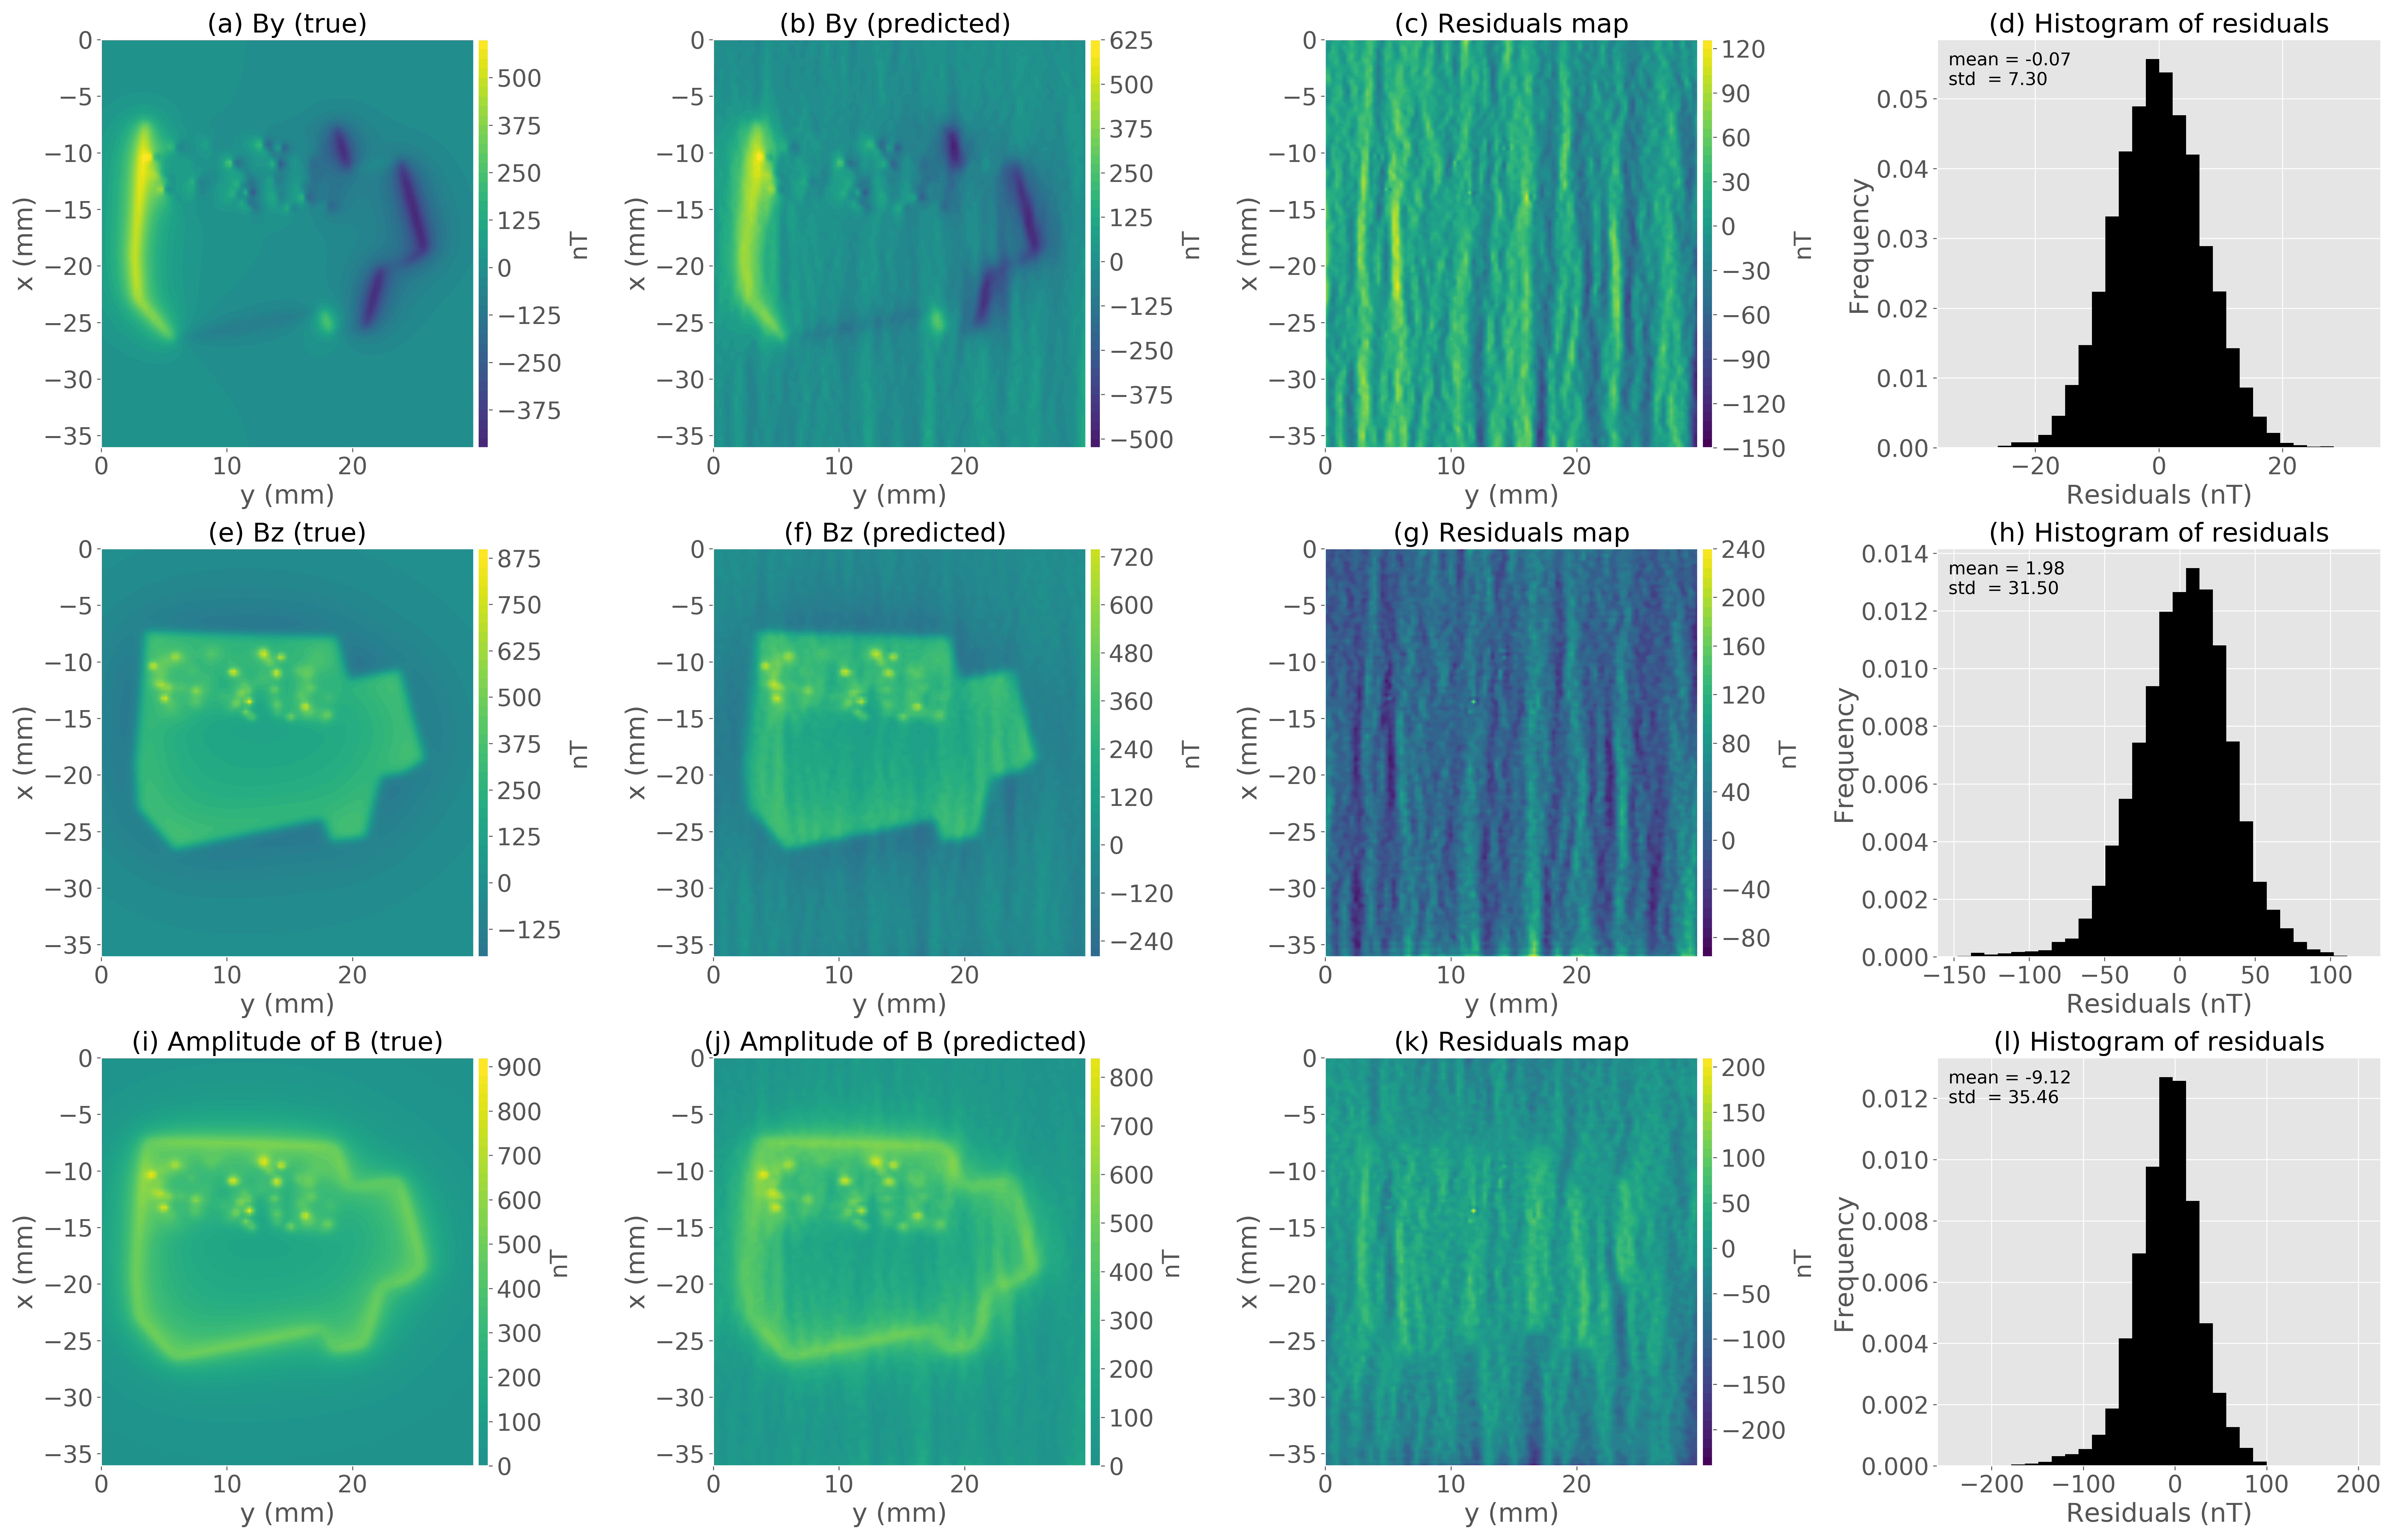
\includegraphics[width=1.15\textwidth]{Fig/mag_vec/simulacao_real_correto/comparison_true_estimated.png}
	\caption{Aplicação a dados sintéticos para a amostra heterogênea com a mesma direção de magnetização da camada equivalente. (a),(e) e (i) Componentes $x$, $y$ e a amplitude verdadeiras do campo magnético, respectivamente. (b), (f) e (j) Componentes $x$, $y$ e a amplitude do campo magnético preditas pela camada equivalente, respectivamente. (c), (g) e (k) Mapas dos resíduos. (d), (h) e (l) Histograma dos resíduos.}
	\label{fig:comparison_hetero_sample_samedir}
\end{figure}


\subsection{Camada equivalente com direção de magnetização diferente da amostra}
\label{subsec:hetero_dif_dir}

Utilizamos uma camada equivalente composta por um grid de $121 \times 99$ posicionados a uma profundidade de $z_c = 868$ microns abaixo do plano de observação. 
A direção de magnetização para as fontes equivalente foi de $40^\circ$ para a inclinação e $50^\circ$ para a declinação, enquanto a amostra possui $90^\circ$ para a inclinação e $0^\circ$ para a declinação. 
Utilizando a equação \ref{eq:linear_sys_p_alpha}, estimamos a distribuição de momentos magnéticos (não mostrada). 
A Figura \ref{fig:datafit_hetero_sample_difdir}b mostra os dados preditos produzidos pela camada equivalente. 
A Figura \ref{fig:datafit_hetero_sample_difdir}c mostra os resíduos definidos pela diferença entre os dados simulados (Figura \ref{fig:datafit_hetero_sample_difdir}a) e os dados preditos (Figura \ref{fig:datafit_hetero_sample_difdir}b). Os resíduos aparecem com distribuição normal de média $-0,2 \, nT$ e desvio padrão $16,07 \, nT$ como mostrado na figura \ref{fig:datafit_hetero_sample_difdir}d. Com a distribuição de momentos magnéticos estimada, conseguimos calcular as componentes e a amplitude do campo magnético com as equações \ref{eq:B-alpha-pred-i}--\ref{eq:Mij-matrix-alpha} e \ref{eq:amplitude_field} (Figura \ref{fig:components_hetero_sample_difdir}a-d). Com o objetivo de verificarmos se a camada equivalente produziu as componentes e a ampĺitude do campo magnético com sucesso, calculamos os valores verdadeiros que são mostrados nas Figuras \ref{fig:comparison_hetero_sample_difdir}a, \ref{fig:comparison_hetero_sample_difdir}e e \ref{fig:comparison_hetero_sample_difdir}i. As figuras \ref{fig:comparison_hetero_sample_difdir}b, \ref{fig:comparison_hetero_sample_difdir}f e \ref{fig:comparison_hetero_sample_difdir}j são os dados preditos pela camada equivalente. 
As Figuras \ref{fig:comparison_hetero_sample_difdir}c, \ref{fig:comparison_hetero_sample_difdir}g e \ref{fig:comparison_hetero_sample_difdir}k são resíduos entre os dados verdadeiros e os dados preditos pela camada. As figuras \ref{fig:comparison_hetero_sample_difdir}d, \ref{fig:comparison_hetero_sample_difdir}h e \ref{fig:comparison_hetero_sample_difdir}l são os histogramas dos resíduos. Apesar da camada equivalente ter direção de magnetização muito diferente da direção da amostra e também a presença de dipolos interferentes, as estimativas para as componentes e a amplitude do campo magnético foram próximas as verdadeiras. Podemos concluir que a distribuição de momentos magnéticos estimada produziu um bom ajuste dos dados.   

%%%% Figuras 

\begin{figure}
	\centering
	
\includegraphics[width=.9\textwidth]{Fig/mag_vec/simulacao_real_errado/results_data_fitting_Bz.png}
	\caption{Aplicação a dados sintéticos para a amostra heterogênea com direção de magnetização diferente da camada equivalente. (a) Componente vertical observada. (b) Dados preditos produzido pela camada equivalente. (c) Diferença entre os dados mostrados nos gráficos a e b. (d) Histograma dos resíduos.}
	\label{fig:datafit_hetero_sample_difdir}
\end{figure}

\begin{figure}
	\centering
	\includegraphics[width=1.\textwidth]{Fig/mag_vec/simulacao_real_errado/field_components_eqlayer.png}
	\caption{Aplicação a dados sintéticos para a amostra heterogênea com direção de magnetização diferente da camada equivalente. (a) Componente vertical predita pela camada. (b) Componente $x$ do campo magnético predita pela camada. (c) Componente $y$ do campo magnético predita pela camada. (d) Amplitude do campo magnético calculado através da equação \ref{eq:amplitude_field}.}
	\label{fig:components_hetero_sample_difdir}
\end{figure}

\begin{figure}
	\centering
	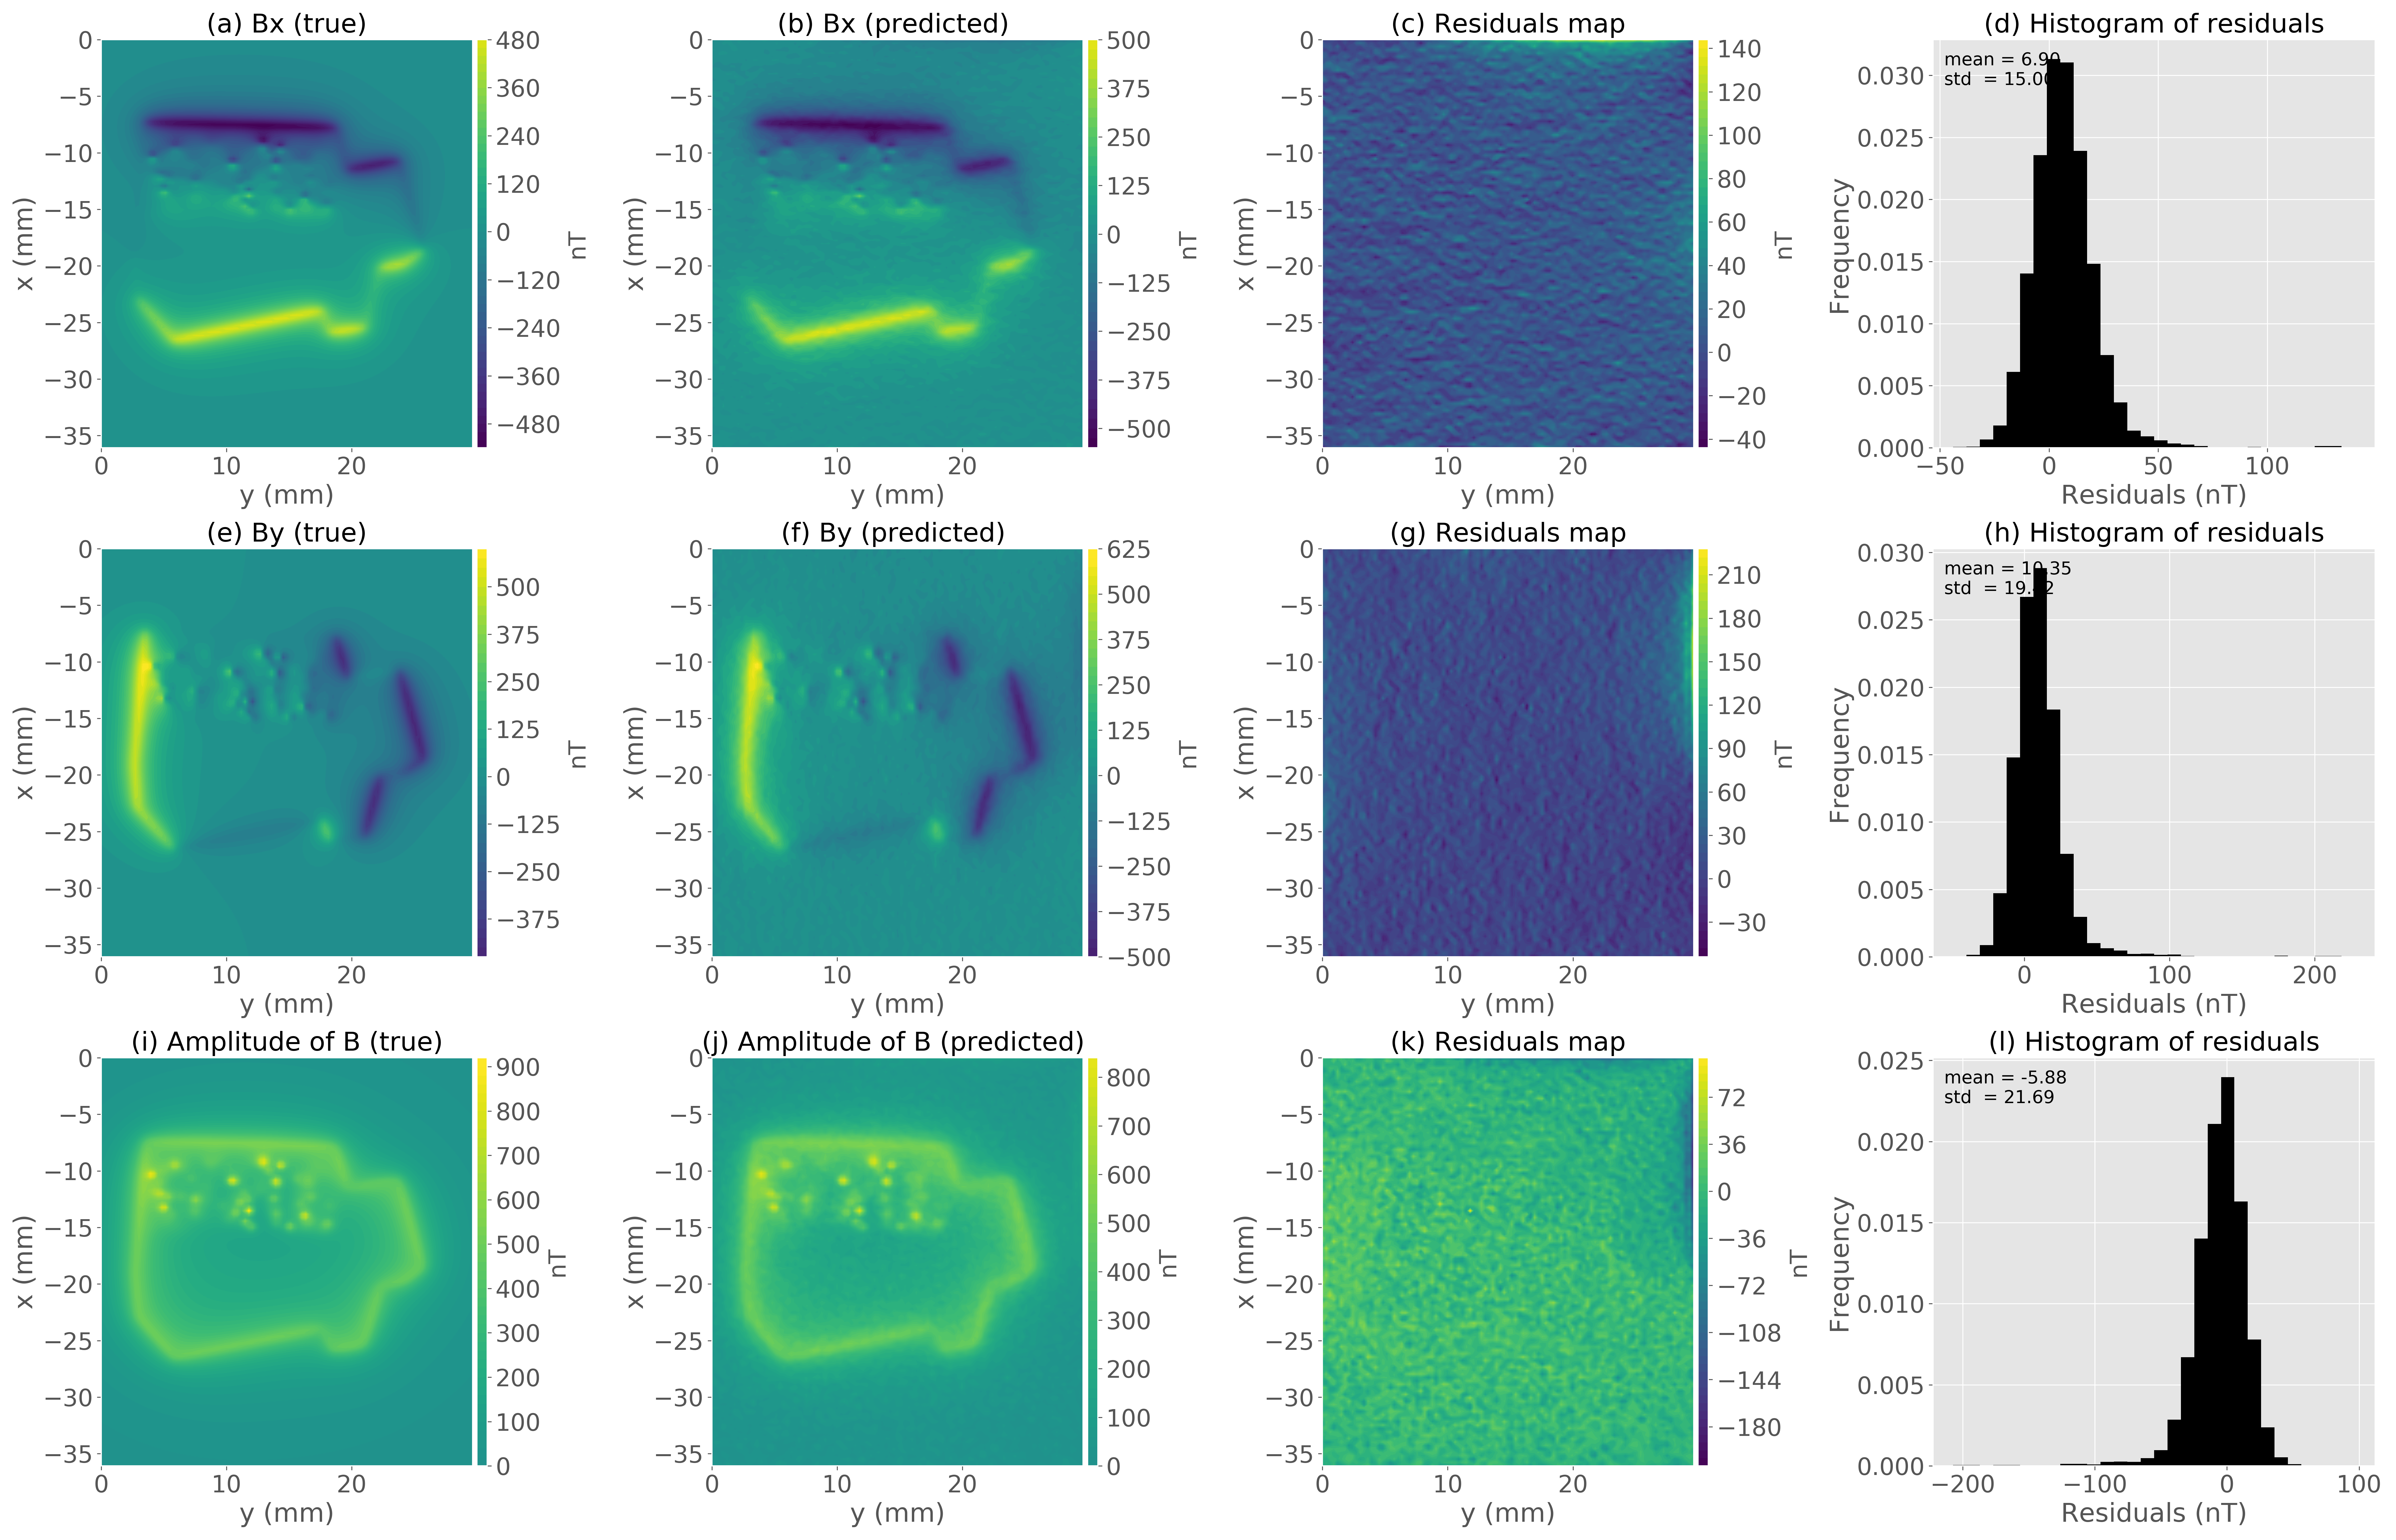
\includegraphics[width=1.15\textwidth]{Fig/mag_vec/simulacao_real_errado/comparison_true_estimated.png}
	\caption{Aplicação a dados sintéticos para a amostra heterogênea com direção de magnetização diferente da camada equivalente. (a),(e) e (i) Componentes $x$, $y$ e a amplitude verdadeiras do campo magnético, respectivamente. (b), (f) e (j) Componentes $x$, $y$ e a amplitude do campo magnético preditas pela camada equivalente, respectivamente. (c), (g) e (k) Mapas dos resíduos. (d), (h) e (l) Histograma dos resíduos.}
	\label{fig:comparison_hetero_sample_difdir}
\end{figure}



%% Dados reais: Cratera de Vredefort
%\chapter{Aplicação a dados de laboratório: amostra da cratera de Vredefort}
\label{sec:lab_application}

Uma cratera de impacto é o registro de um dos processos geológicos mais rápidos já conhecidos. As altas pressões ($> 5$ GPa) e as altas temperaturas ($> 1000^\circ$C) de choque são responsáveis pela formação de sistemas geoquímicos únicos. A evolução de tais sistemas podem gerar assinaturas petrofísicas complexas \citep{pilkington_grieve_1992,pilkington_hildebrand_2003,yokoyama_etal_2015}. Um exemplo destas assinaturas pode ser observado em dados magnéticos do domo de Vredefort, na África do Sul. O domo de Vredefort é uma das mais extensas estruturas de impacto já conhecida na Terra, com um diâmetro de aproximadamente $250$ km, de forma que estudos magnéticos tem sido realizados desde os anos 60. Esta estrutura possui diversos tipos de impactitos, tais como veios de impacto, diques com estrutura granofírica e \textit{shatter cones}. Neste contexto, estudos paleomagnéticos são recorrentes em veios de impactos, especialmente os pseudotaquilitos. Estas rochas são escuras e vítreas formadas, principalmente, por forte fricção. Elas são encontradas em zonas de falha e cisalhamentos, e em algumas estruturas de impacto tais como o domo de Vredefort. Portanto, neste trabalho, foi utilizada uma amostra da região de Leeukop Quarry no domo de Vredefort \citep{araujo_etal2019_materials}, similar às usadas em outros estudos paleomagnéticos \citep{passchier_1982,lana_etal_2003,dressler_reimold_2004,carporzen_etal_2005,araujo_etal2019_sensors}. Na Figura \ref{fig:datafit_real_sample}a apresentamos o mapa de microscopia magnética da amostra de Vredefort. Estas medidas foram realizadas em ambiente com blindagem para campos magnéticos de até $15$ mT. Além disso, aplicamos um campo magnético de $400$ mT na direção do eixo $z$. Os dados foram medidos em um grid regular de $121 \times 99$ pontos (um total de $N=11979$ observações) sobre uma área que se estende em $36$ mm e $30$ mm ao longo dos eixos $x$ e $y$, respectivamente. A distância sensor-amostra foi igual a $138$ microns acima da superfície da amostra. 


Para a inversão, utilizamos uma camada equivalente formada por um grid de $121 \times 99$ dipolos (um total de $M=11979$ fontes equivalentes) posicionadas a uma profundidade constante de $z_c = 818$ microns abaixo da superfície de observação. A direção de magnetização para os dipolos é igual a $90^\circ$ para a inclinação e $0^\circ$ para a declinação, que é a mesma direção do campo aplicado na amostra. Resolvendo a equação \ref{eq:linear_sys_p_alpha}, estimamos a distribuição de momentos magnéticos sobre a camada equivalente (não mostrado). A figura \ref{fig:datafit_real_sample}b mostra os dados preditos produzidos pela camada equivalente. Na figura \ref{fig:datafit_real_sample}c é apresentado o mapa dos resíduos, que é definido como a diferença entre os dados observados (Figura \ref{fig:datafit_real_sample}a) e os dados preditos (Figura\ref{fig:datafit_real_sample}b). O histograma dos resíduos aparece com média de $0$ mT e desvio padrão de $0,03$ mT (Figura \ref{fig:datafit_real_sample}d). Isto significa que a distribuição de momentos magnéticos produziu um ajuste aceitável dos dados observados. As componentes e a amplitude do campo magnético preditas pela camada equivalente são mostradas nas figuras \ref{fig:components_real_sample}a, \ref{fig:components_real_sample}b, \ref{fig:components_real_sample}c e \ref{fig:components_real_sample}d. O resultado apresentado na figura \ref{fig:components_real_sample}d mostra uma concentração de minerais magnéticos na borda superior da amostra de Vredefort. Com os resultados apresentados, podemos concluir que a técnica da camada equivalente pode ser uma ferramenta útil para o processamento de dados magnéticos, de forma que conseguimos calcular as componentes do campo magnético e sua amplitude sem termos conhecimento prévio da direção de magnetização da fonte magnética. 

%%% Figuras para aplicação a dados reais 
\begin{figure}
	\centering
	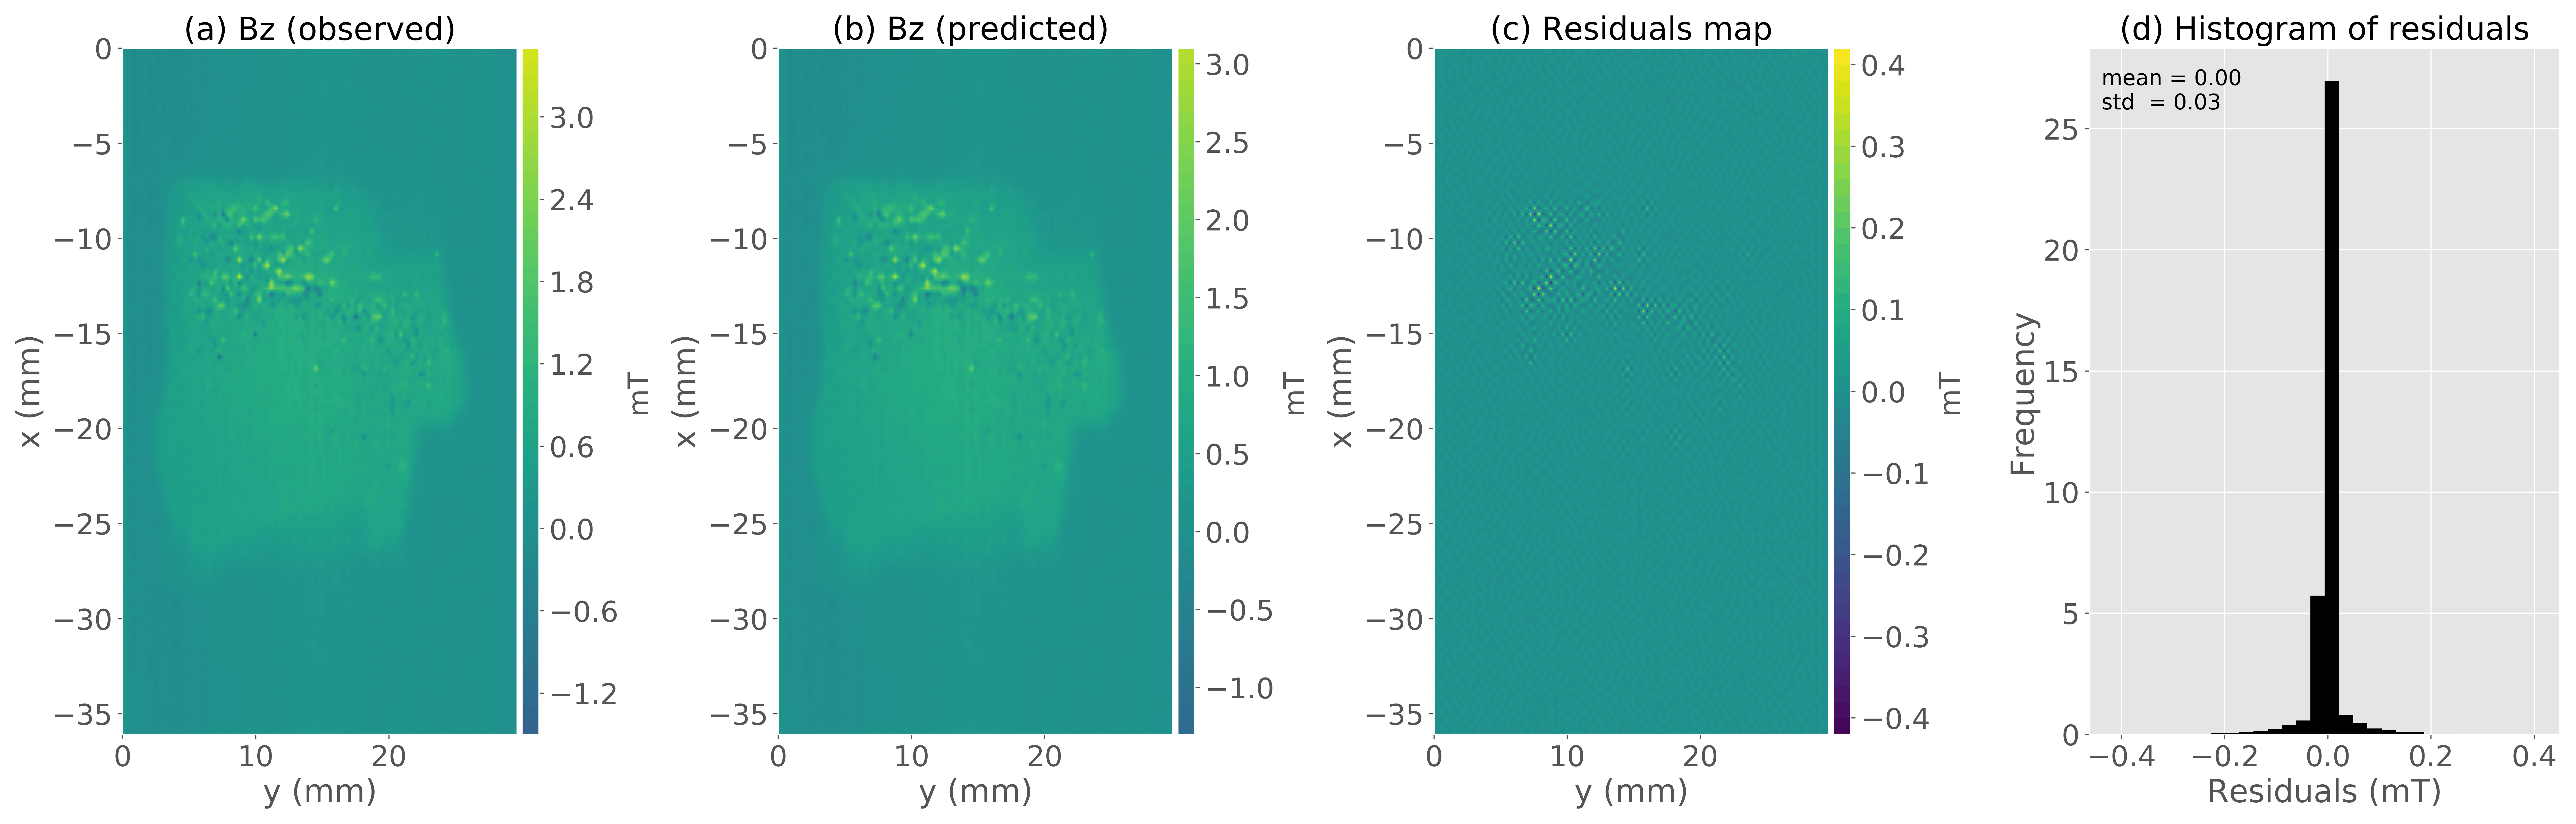
\includegraphics[width=.9\textwidth]{Fig/mag_vec/aplicacao_vredefort/results_data_fitting_Bz.png}
	\caption{Aplicação a dados de laboratório para a amostra de Vredefort. (a) Componente vertical observada. (b) Dados preditos produzido pela camada equivalente. (c) Diferença entre os dados mostrados nos gráficos a e b. (d) Histograma dos resíduos.}
	\label{fig:datafit_real_sample}
\end{figure}

\begin{figure}
	\centering
	\includegraphics[width=1.\textwidth]{Fig/mag_vec/aplicacao_vredefort/field_components_eqlayer.png}
	\caption{Aplicação a dados de laboratório para a amostra de Vredefort. (a) Componente vertical predita pela camada. (b) Componente $x$ do campo magnético predita pela camada. (c) Componente $y$ do campo magnético predita pela camada. (d) Amplitude do campo magnético calculado através da equação \ref{eq:amplitude_field}.}
	\label{fig:components_real_sample}
\end{figure}



%\part{Generalização do vínculo de positividade em camadas equivalentes magnéticas}
%\begin{abstract}
It is known from potential theory that a continuous and planar layer of dipoles can exactly reproduce the total-field anomaly produced by arbitrary 3D sources. We show that, if the magnetization direction of this layer is the same as that of the true sources, its magnetic-moment distribution is all positive. This property holds true regardless of whether the magnetization of the true sources is purely induced or not. By using this generalized positivity constraint, we present a new iterative method for estimating the total magnetization direction of 3D magnetic sources based on the equivalent-layer technique. Our method does not impose a priori information either about the shape or depth of the sources, does not require regularly spaced data and presumes that the sources have a uniform magnetization direction. At each iteration, our method performs two steps. The first one solves a constrained linear inverse problem to estimate a positive magnetic-moment distribution over a discrete equivalent layer of dipoles. We consider that the equivalent sources are located on a plane and have an uniform and fixed magnetization direction. The second step uses the estimated magnetic-moment distribution and solves a nonlinear inverse problem for estimating a new magnetization direction for the dipoles. The algorithm stops when the equivalent layer yields a total-field anomaly that fits the observed data. Tests with synthetic data simulating different geological scenarios show that the final estimated magnetization direction is close to the true one. We applied our method to a field data from the Goi{\' a}s Alkaline Province (GAP), over the Montes Claros complex, center of Brazil. The result suggests the presence of intrusions with remarkable remanent magnetization, in agreement with the current literature for this region.
\end{abstract}   
%\section{Conclusion}
\label{sec:conclusion}

We have shown mathematically that the total-field anomaly data caused by a set of magnetic sources
with uniform magnetization direction can be exactly reproduced by a continuous and planar layer of 
dipoles having an all-positive magnetic-moment distribution. 
This theoretical property holds true for the case in which the layer has the same
magnetization direction as that of the true sources, regardless of whether they have 
a purely induced magnetization or not.
By using this generalized positivity constraint, we have presented a new iterative method for 
estimating the total magnetization direction of 3D magnetic sources based on the equivalent-layer technique. 
At each iteration, we impose a positivity constraint on the estimated magnetic-moment distribution of the layer 
and solves a non-linear inverse problem for estimating the magnetization direction of the equivalent sources. 
Prior knowledge about the shape and depth of magnetic sources are not required, neither the use of an evenly spaced 
data set. This methodology can be applied for determining the magnetization direction of multiple sources, 
considering all of them with the same magnetization direction. 
Results obtained with synthetic data produced by multiple sources have shown that the estimated magnetization direction 
obtained by our iterative method successfully retrieves the true one.
Tests with synthetic data have also illustrated how the presence of a relatively shallow-seated source affects the 
result obtained by our method for the cases in which it has a magnetization direction equal to and different from 
the other sources. In both cases, the equivalent layer yielded large data misfits above the shallow source;
however, we cannot distinguish if the shallow source has a magnetization direction equal or different from the other sources. 
Moreover, our method produces the worst estimated magnetization direction when shallow-seated source is magnetized in a 
direction that differs from the other sources.
An application to field data over the Goi{\' a}s alkaline province, center of Brazil, has confirmed that our method can 
be a reliable tool for interpreting complex geological scenarios. The result over the Montes Claros complex suggests the presence 
of a strong remanent magnetization component and corroborates a previous study conducted independently at the same area. 
The estimated magnetic-moment distribution over the layer has led to a very acceptable reduction to the pole, but have also 
produced large data-misfits at some isolated regions. We presume that these locally large data-misfits are due to shallow sources, 
however we cannot infer if they have the same magnetization direction of the other bodies.   


%% Apêndices A e B 
\appendix
\chapter{Dedução da equação \ref{eq:positivity_prop}}
\label{append:proof-positive-p}

Neste apêndice, provamos a existência da distribuição de momentos magnéticos positiva $p(x'', y'', z_{c})$ que resolve a integral apresentada na equação \ref{eq:Omega-tilde-potential}. 

Considere a superfície fechada localizada acima das fontes magnéticas, formada por um plano $z = z_{c}$ contendo a camada equivalente e uma semi-esfera com radio infinito (Figura \ref{fig:surface_Green}). Esta superfície cerca a região na qual  $\Gamma(x'', y'', z_{c})$ (equação \ref{eq:Gamma-volume-integral}) é uma função harmônica. Utilizando a segunda indentidade de Green \citep[][ p. 215]{kellogg1967}, mostramos que 

\begin{equation}
0 = \frac{1}{4\pi}
\int\limits_{-\infty}^{+\infty}\int\limits_{-\infty}^{+\infty}
\partial_{z} \Gamma(x'', y'', z_{c}) \: \frac{1}{\ell} - 
\Gamma(x'', y'', z_{c}) \: \partial_{z} \frac{1}{\ell}
\:\: dS'' \: , \quad z_{c} > z \: ,
\label{eq:Greens_2nd_identity}
\end{equation}
em que $\Gamma(x'', y'', z_{c})$ é a integral de volume definida pela equação \ref{eq:Gamma-volume-integral} e 

\begin{equation}
\frac{1}{\ell} \equiv \frac{1}{\sqrt{(x - x'')^{2} +
		(y - y'')^{2} +
		(z_{s} - z_{c})^{2}}}
\label{eq:inv-l}
\end{equation}
é o inverso da distância entre o ponto fixo $(x'', y'', z_{c})$, localizado sobre a camada equivalente, e o ponto $(x, y, z_{s})$, com $z_{s} = z_{c} + \Delta z$, $\Delta z > 0$. 

O ponto $(x, y, z_{s})$ é convenientemente definido como o espelho do ponto $(x, y, z)$, localizado em $z = z_{c} - \Delta z$, com respeito ao plano $z = z_{c}$ que contém a camada equivalente (Figura \ref{fig:surface_Green}). A equação \ref{eq:Greens_2nd_identity} combinada com a terceira identidade de Green \citep[][ p. 219]{kellogg1967} nos fornece como resultado 

\begin{equation}
\Gamma(x, y, z) = \frac{1}{4\pi}
\int\limits_{-\infty}^{+\infty}\int\limits_{-\infty}^{+\infty}
\partial_{z} \Gamma(x'', y'', z_{c}) \: 
\left( \frac{1}{r} + \frac{1}{\ell} \right)
\Gamma(x'', y'', z_{c}) \: 
\left( \partial_{z} \frac{1}{r} + \partial_{z} \frac{1}{\ell} \right)
\:\: dS'' \: , \quad z_{c} > z \: ,
\label{eq:Greens_3rd_identity}
\end{equation}
em que $\frac{1}{r}$ é definida pela equação \ref{eq:inverse-distance}. O termo $\left( \frac{1}{r} + \frac{1}{\ell} \right)$ representa a \textit{função de Green de segunda ordem} \citep[][ p. 246]{kellogg1967} associada a esta integral. 

Note que $\frac{1}{r} = \frac{1}{\ell}$, $\partial_{z} (1/r) = -\partial_{z} (1/\ell)$ e, consequentemente, 

\begin{equation}
\Gamma(x, y, z) = \frac{1}{2\pi}
\int\limits_{-\infty}^{+\infty}\int\limits_{-\infty}^{+\infty}
\partial_{z} \Gamma(x'', y'', z_{c}) \: \frac{1}{r} 
\:\: dS'' \: , \quad z_{c} > z \: .
\label{eq:Neumann_bvp}
\end{equation}
Esta equação mostra que a ambiguidade inerente a campos potenciais \citep{roy1962} e resolve o \textit{problema de Neumann} ou o \textit{problema de contorno de segunda ordem da teoria do potencial} \citep[][ p. 246]{kellogg1967}. Neste caso, este problema consiste em definir a função harmônica $\Gamma(x, y, z)$ (equação \ref{eq:Gamma-volume-integral}) na região acima da camada equivalente, a partir dos valores de suas derivadas verticais sobre o plano que contém a camada. 

%% Figura 

\begin{figure}
	\centering
	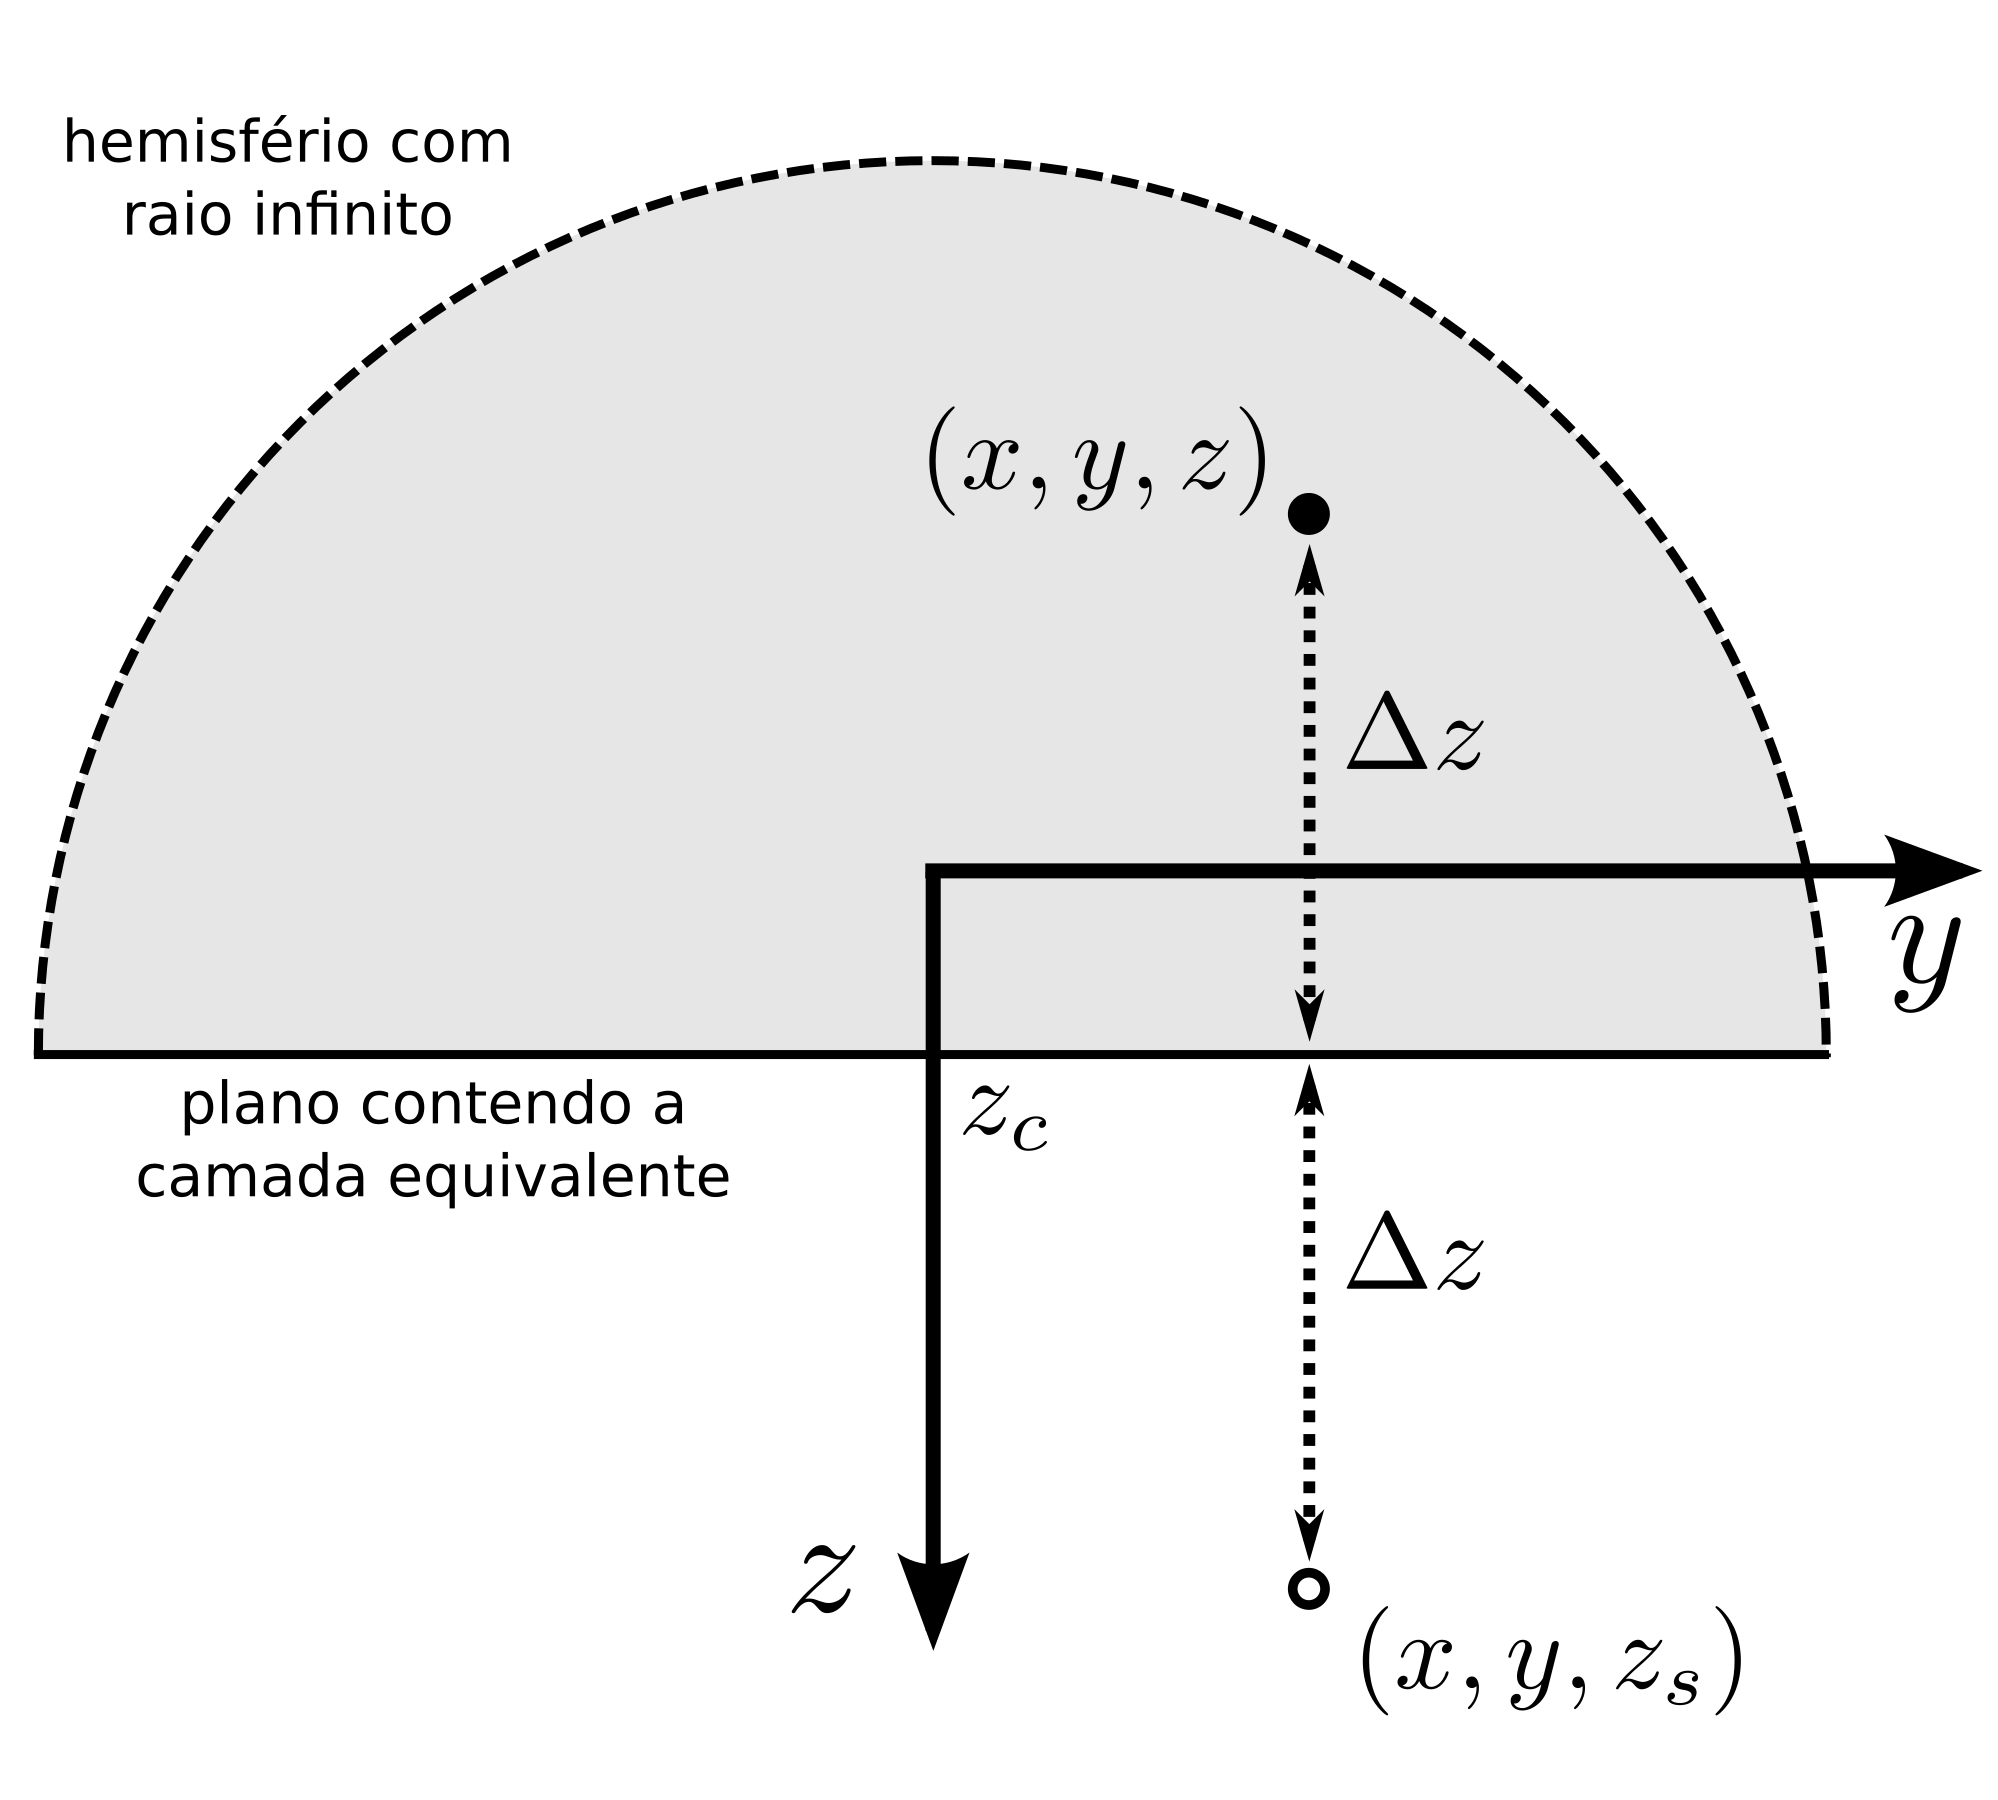
\includegraphics[width=0.75\textwidth]{Fig/eqlayer/surface_Green.png}
	\caption{ Representação 2D da superfícia utilizada para aplicar as identidades de Green. A superfície é formada por uma semi-esfera (linha traçejada) com raio infinito e o plano $z = z_{c}$ contendo a camada equivalente. Os pontos $(x, y, z)$ (ponto fechado) e $(x, y, z_{s})$ (ponto aberto) são posicionados simetricamente com respeito ao plano $z = z_{c}$ e definidos como $z = z_{c} - \Delta z$ e $z = z_{c} + \Delta z$, respectivamente.}
	\label{fig:surface_Green}
\end{figure}
\chapter{Fontes magnetizadas verticalmente}
\label{append:vertical-magnetization}

Nosso método falha quando a magnetização total das fontes possui a direção igual ou aproximadamente vertical. Neste apêndice, fornecemos a base teórica para o entendimento desta limitação. 

Considere o caso limite no qual a magnetização total das fontes é vertical e.g., $I = \pm 90^\circ$). Neste caso, a anomalia de campo total $\Delta T(x, y, z)$ (equação \ref{eq:tfanomaly}) não depende da declinação $D$, demonstrado pelo fato que: fontes magnetizadas verticalmente não possuem uma declinação definida. Consequentemente, o mínimo da função objetivo (equação \ref{eq:positivity_goal_function}a) não é bem definida no espaço dos parâmetros; isto é, ela é alongada na direção de $D$. Infelizmente, o vínculo de positividade sobre o vetor de momentos magnéticos (equação  \ref{eq:positivity_goal_function}b) não resolve esta ambiguidade com respeito a declinação $D$. 

Para melhor entender como esta ambiguidade afeta nosso método, começamos a analisar a matriz $\mathbf{G}_{q}^{k}$ de dimensão $N \times 2$ (equação \ref{eq:Gq}) necessária para estimar a correção $\bar{\mathbf{\Delta q}}^{k}$ para a direção de magnetização (equação \ref{eq:linear_sys_q}). Sua $i$-ésima linha é definida como o produto do vetor de momentos magnéticos estimado $\bar{\mathbf{p}}^{k}$ e as primeiras derivadas $\partial_{\alpha} \mathbf{g}_{i}(\bar{\mathbf{q}}^{k}) \equiv 
\frac{\partial \mathbf{g}_{i}(\bar{\mathbf{q}}^{k})}{\partial \alpha}$, $\alpha= I, D$, do vetor $\mathbf{g}_{i}(\mathbf{q})$ (equação \ref{eq:tfa_pred_i}), avaliada em $\mathbf{q} = \bar{\mathbf{q}}^{k}$, com respeito a inclinação $I$ e a declinação $D$ da magnetização total das fontes. O $j$-ésimo elemento $\partial_{\alpha} g_{ij}(\bar{\mathbf{q}}^{k}) \equiv 
\frac{\partial g_{ij}(\bar{\mathbf{q}}^{k})}{\partial \alpha}$ do vetor $\partial_{\alpha} \mathbf{g}_{i}(\bar{\mathbf{q}}^{k})$ de dimensão $M \times 1$ é definido como a derivada da função harmônica $g_{ij}(\mathbf{q})$ (equação \ref{eq:g_ij}) igual a 

\begin{equation}
\partial_{\alpha} g_{ij}(\bar{\mathbf{q}}^{k}) = 
\gamma_m  \hat{\mathbf{F}}_{0}^T \, \mathbf{M}_{ij} 
\partial_{\alpha} \hat{\mathbf{m}}(\bar{\mathbf{q}}^{k}) \: , \quad \alpha = I, D \: ,
\label{eq:D-alpha-gij}
\end{equation}
em que 

\begin{equation}
\partial_{I} \hat{\mathbf{m}}(\bar{\mathbf{q}}^{k}) = 
\begin{bmatrix}
	-\sin \bar{I}^{k} \cos \bar{D}^{k} \\
	-\sin \bar{I}^{k} \sin \bar{D}^{k} \\
	 \cos \bar{I}^{k}
\end{bmatrix}
\label{eq:D_mag_vec_inc}
\end{equation}
e 

\begin{equation}
\partial_{D} \hat{\mathbf{m}}(\bar{\mathbf{q}}^{k}) = 
\begin{bmatrix}
	-\cos \bar{I}^{k} \sin \bar{D}^{k} \\
	 \cos \bar{I}^{k} \cos \bar{D}^{k} \\
	 0
\end{bmatrix}
\label{eq:D_mag_vec_dec}
\end{equation}
são as derivadas do vetor unitário $\hat{\mathbf{m}}(\mathbf{q})$ (equação \ref{eq:mag_vet}), avaliadas na direção de magnetização $\bar{\mathbf{q}}^{k} = \left[ \bar{I}^{k} \:\: \bar{D}^{k} \right]^{\top}$, com respeito a $I$ e $D$. 
 
Note que, quando a inclinação estimada $\bar{I}^{k}$ se aproxima de $\pm 90^{\circ}$, todos os elementos que formam o vetor  $\partial_{D} \hat{\mathbf{m}}(\bar{\mathbf{q}}^{k})$ (equação \ref{eq:D_mag_vec_dec})e, consequentemente, a segunda coluna da matriz $\mathbf{G}_{q}^{k}$ (equação \ref{eq:Gq}) tendem a zero. Como consequência, o problema não-linear para estimar a direção de magnetização (equação \ref{eq:linear_sys_q}) não é sensível a mudanças na declinação $D$ e a convergência do nosso método é muito lenta devido a suavidade da função objetivo $\Psi(\mathbf{s})$ (equação \ref{eq:positivity_goal_function}a) no espaço de parâmetros. 



\backmatter

% estilo de citações por ordem alfabética (defaut da classe ONTeX)
\bibliographystyle{on-plain}
\bibliography{references.bib}

  
\end{document} 